% !TeX program = pdflatex
% Компиляция: bash build_paper.sh  (pdflatex прогоняется до схождения
% перекрёстных ссылок; двух проходов не хватает, нужно три)
%
% ВЕРСИЯ 2. Работа переведена с моментного вывода схемы B на ТОЧНЫЙ
% условный вывод: K_b = N_b - 1 | D_b ~ Poisson(lambda_b D_b).
% Все числовые значения — вывод analysis_v2.py при зерне 20260914
% (results_v2.txt, теги [S0]...[S12]).
%
% ВЕРСИЯ 3 (редакция 24.09.2026). Изменения по существу:
%  * предложение о точном условном законе переформулировано как УСЛОВНОЕ
%    ПРАВДОПОДОБИЕ: D_b достаточна для W_b при фиксированной kappa
%    (факторизация); показано совпадение с интегрированным правдоподобием
%    при мере dW_b (мера Хаара сдвигов) и связь с задачей Неймана — Скотта;
%  * условие (A1) сформулировано для СЛУЧАЙНОГО окна, независимого от процесса;
%  * «доказуемая двусторонняя вилка» [(M-B)/S, (M-1)/S] ОТОЗВАНА: без (A1)
%    строго держится лишь верхняя граница (тождество Вальда); правило
%    остановки «после долгой засухи» даёт смещение (M-B)/S вверх
%    (новый тег [S13], скрипт stopping_rules.py);
%  * исправлен множитель смещения МНК при схеме B (две разные регрессии);
%  * неверная ссылка на Pomerance 1981 (псевдопростые) заменена на
%    Math. Intelligencer 3 (1981) 97-105;
%  * мелкие численные уточнения (покрытие Гарвуда, p однородности,
%    (1+mu)e^{-mu} при mu=16, число событий в расчёте мощности);
%  * НОВЫЙ раздел sec:second: член второго порядка самой эвристики ЛПВ,
%    lambda_b(t) = (kappa/ln b)(1 + c_b/t), точный условный вывод при заданном c
%    (lpw_second_order.py, теги [S14]-[S17], вывод в results_v3.txt);
%  * закрыты все маркеры \recompute (модель eq:logcorr, B=20, исключение по
%    одному основанию);
%  * НОВЫЙ подраздел sec:frontiers: документированные фронты b=2,10,22,26,
%    эмпирическая проверка (A1) и гибридная оценка (frontiers.py, тег [S18]);
%    отмечены PRP R_5(4939471), R_5(5154509) 2024 г. вне OEIS.
%
% ВЕРСИЯ 3.1 (редакция 30.09.2026, по редакторскому заключению и трём рецензиям):
%  * sec:second: экспозиция члена второго порядка СУММИРУЕТСЯ ПО ПРОСТЫМ, а не
%    интегрируется с плотностью 1/ln n (lpw_prime_sum.py, теги [S26]-[S28]);
%    интеграл завышал экспозицию у нижнего конца окна на постоянную Мертенса E
%    и занижал оценку на 9,0% (полная выборка) и 3,8% (n>10). Исправлены
%    таблица tab:second, выводы (i)-(v), аннотация, п. 7 вклада и заключения;
%    вывод <<член второго порядка снимает убывание при усечении>> отозван;
%    рисунок fig:truncation перестроен;
%  * sec:robust: <<это тренд, а не шум>> заменено вероятностями при схемах A и B;
%    добавлены начало отсчёта в точке усечения и арифметически заданное начало
%    n_min = 2; общий заведомо пройденный фронт 2e5 (robust_extra.py, [S29]);
%  * основание 18 (sec:instability), замечание о независимости, подпись рис. 4,
%    нулевой закон sec:sameerror и броуновский мост, sec:second <<знак свободного
%    члена>> (симуляция вместо грубой оценки -1,98), пороги мощности для
%    занижения, исключение оснований-степеней, фронт GIMPS после 4.09.2026.
%
% ВЕРСИЯ 3.2 (редакция 01.10.2026, по решению редактора о существенной доработке):
%  * аннотация, п. 4--5 вклада и заключение переписаны в условной форме: вывод
%    <<превышение создаётся схемой наблюдения>> держится на (A1), а вывод <<ЛПВ не
%    отвергается>> устойчив ко всему семейству (M-Bm)/S (таблица tab:mfamily);
%  * таблица tab:stop: частичное нарушение (A1), столбцы m и уровень сдвинутого
%    критерия; новое замечание rem:weaker о фактическом и опубликованном фронте;
%  * sec:frontiers: несинхронные фронты как нижние границы, отбор оснований;
%  * точность закона (12) отнесена к модели (3), пуассон-биномиальный закон в
%    модели Бернулли; совместный интервал sec:second (v) --- смесь Гарвуда;
%  * чувствительность к пропускам поиска, статус PRP, атрибуция табл. tab:verify,
%    протокол двойного счёта; мелкие правки по всем замечаниям рецензентов
%    (revision_v32.py, тег [S30]; stopping_rules.py, тег [S13]).
\documentclass[11pt,a4paper]{article}

% cmap ДОЛЖЕН идти до fontenc: он встраивает в PDF таблицы ToUnicode, без
% которых кириллица не извлекается из готового файла — текст нельзя ни найти
% поиском, ни скопировать, ни разобрать системам индексации (РИНЦ, Crossref).
\usepackage{cmap}
\usepackage[T2A]{fontenc}
\usepackage[utf8]{inputenc}
\usepackage[english,russian]{babel}
\usepackage{amsmath,amssymb,amsthm}
\usepackage{booktabs}
\usepackage{graphicx}
% Рисунки генерирует analysis_v2.py и кладёт в figs_v2/ (figs/ -- рисунки v1).
\graphicspath{{figs_v2/}}
\usepackage[margin=25mm]{geometry}
% xurl ДО hyperref: разрешает переносить длинные URL в любом месте. Без него
% ссылки вроде t5k.org/mersenne/heuristic.html вылезают за правое поле.
\usepackage{xurl}
\usepackage[colorlinks=true,allcolors=blue]{hyperref}
% Запас на растяжение межсловных пробелов: в русском тексте с большим числом
% неразрывной формульной вёрстки без него остаются переполненные строки.
\emergencystretch=3em
\usepackage{xcolor}
\usepackage[expansion=false]{microtype}
% Подписи в принятом отечественном виде: «Рис. 1. Название», «Таблица 1. Название»
% (вместо «Рис. 1: Название»).
\usepackage{caption}
\captionsetup{labelsep=period}
% п. 4.1.5 ГОСТ Р 7.0.7-2021: подписи к иллюстративному материалу приводят на
% языке текста статьи и, как правило, повторяют на английском языке.
% Номер берётся из счётчика, уже увеличенного \caption, поэтому русская и
% английская подписи всегда несут один и тот же номер.
\newcommand{\encaptab}[1]{\\[3pt]\foreignlanguage{english}{%
  \textbf{Table~\thetable.} #1}}
\newcommand{\encapfig}[1]{\\[3pt]\foreignlanguage{english}{%
  \textbf{Figure~\thefigure.} #1}}

% Маркер величин, которые НЕЛЬЗЯ получить из троек (N_b, n_min, n_max) и
% которые требуют полных списков индексов: они пересчитываются
% analysis_v2.py при наличии b-файлов (ключ --oeis-dir). Перед подачей
% запустить скрипт с данными и заменить маркеры на числа; команду
% переопределить пустой, чтобы убедиться, что маркеров не осталось.
\newcommand{\recompute}[1]{\textcolor{red}{[пересчитать: #1]}}

\theoremstyle{plain}
\newtheorem{proposition}{Предложение}
\newtheorem{corollary}{Следствие}
\theoremstyle{remark}
\newtheorem{remark}{Замечание}

\newcommand{\Rb}{R_b}
\newcommand{\eg}{e^{\gamma}}
\newcommand{\emg}{e^{-\gamma}}
\DeclareMathOperator{\Gam}{Gamma}
\DeclareMathOperator{\Pois}{Poisson}

\title{Схема наблюдения в статистике обобщённых репьюнитных\\
простых: точный условный критерий константы\\
Ленстры --- Померанса --- Вагстаффа}
\author{Тимофей Сергеевич Докучаев\thanks{ORCID: \url{https://orcid.org/0009-0006-0510-5225}.
Контактный адрес: \texttt{timofei93@yandex.ru}}\\
\small Независимый исследователь, Иркутск, Россия}
% Дата фиксирована: \today менялась бы при каждой пересборке.
\date{1 октября 2026~г.}

\begin{document}

% Тип статьи (п. 4.4) и индекс УДК (п. 4.5) ГОСТ Р 7.0.7-2021:
% приводят в начале статьи отдельными строками слева.
\noindent Научная статья\\
\noindent УДК 511.3:519.234
\medskip

% article.cls открывает заголовок командой \newpage — причём дважды: один раз
% в самом \maketitle, второй внутри \@maketitle. Строки «Научная статья» и
% «УДК» к этому моменту уже набраны, поэтому \newpage сбрасывал их отдельной
% страницей, а заглавие уезжало на вторую. Локально обезвреживаем \newpage
% ровно на время \maketitle: строки остаются перед заглавием, как требуют
% пп. 4.4 и 4.5 ГОСТ Р 7.0.7-2021, и всё умещается на первой странице.
\let\RHnewpage\newpage
\let\newpage\relax
\maketitle
\let\newpage\RHnewpage

\begin{abstract}
Эвристика Ленстры --- Померанса --- Вагстаффа (ЛПВ) предсказывает, что
$\#\{n\le x:\Rb(n)\ \text{просто}\}\sim(\eg/\ln b)\ln x$. С 1993~года её проверяют
по <<нормированной частоте встречаемости>>. Цензурирование эту частоту не смещает:
концевая форма и наклон МНК несмещены. Настоящий дефект
иной: формы оценки расходятся до $29{,}5\%$.

Объединяем $B=15$ оснований ($M=218$ событий). Фронты поиска не записаны;
это мешающие параметры Неймана --- Скотта, и профильная оценка $M/S$
несостоятельна. Если фронт выбирался без оглядки на находки (условие (A1)),
положение последней находки $D_b$ достаточно для фронта, и условно на нём
$N_b-1\sim\Pois(\lambda_bD_b)$ точно. Отсюда $(M-B)/S=1{,}838$, точный $95\%$
интервал $[1{,}59;\,2{,}11]$, $p=0{,}67$ против $\eg\approx1{,}781$; старый
критерий отвергает верную гипотезу в $11$--$17\%$ случаев. При (A1)
десятипроцентное превышение над ЛПВ создаётся в основном схемой наблюдения.
Без (A1) согласие с ЛПВ сохраняется при любом среднем зазоре между последней находкой и фронтом от $0$ до
$3{,}2$ средних промежутков ($2{,}8$ с членом второго порядка).

Проверку ЛПВ при конечных $n$ даёт член второго порядка эвристики:
индексу $p$ она приписывает вероятность $\eg\ln(a_bp)/(p\ln b)$. Калибруя
$c_b=\langle\ln a_b\rangle$ по делимости $\Rb(p)$ и суммируя по
простым, при (A1) получаем $1{,}78$ ($1{,}66$--$1{,}78$ при любом усечении,
$p\ge0{,}598$), а
<<медленная сходимость снизу>> получает объяснение.
Критерий однородности ($p=0{,}935$) уверенно различает лишь разброс $\kappa_b$ с
коэффициентом вариации свыше $0{,}37$.

\medskip
\noindent\textbf{Ключевые слова:} репьюнит-простые, обобщённые репьюниты,
числа Мерсенна, гипотеза Ленстры --- Померанса --- Вагстаффа, постоянная
Эйлера --- Маскерони, схема наблюдения, цензурирование типа~I, пуассоновский
точечный процесс, условное правдоподобие, мешающие параметры, задача
Неймана --- Скотта, достаточная
статистика, смещение оценки, мощность критерия, вычислительная теория чисел

\medskip
\noindent\textbf{MSC 2020:} Primary 11Y11; Secondary 11N05, 62F03, 62B05,
62N01, 60G55, 11N80.

\medskip
\noindent\textbf{Благодарности:} автор благодарит проект Great Internet Mersenne
Prime Search (GIMPS) за предоставление данных о простых числах Мерсенна через
открытый отчёт PrimeNet (\url{https://www.mersenne.org/}); значения индексов
Мерсенна получены оттуда 27~августа 2026~года. Автор признателен участникам
OEIS, которые много лет поддерживают последовательности обобщённых репьюнитных
простых. Автор благодарит Jaume Gotanegra (MathOverflow,
\url{https://mathoverflow.net/questions/514719}) за замечание о том, что условное
правдоподобие~\eqref{eq:condlaw} получается также интегрированием по фронту с
мерой $dW_b$ (замечание~\ref{rem:integrated}).

\medskip
\noindent\textbf{Финансирование:} исследование выполнено без внешнего
финансирования.
\end{abstract}

\begin{otherlanguage}{english}

% Англоязычный блок: заглавие, автор, аффилиация, аннотация, ключевые слова.
% Требуется журналами перечня ВАК и всеми индексируемыми в Scopus/WoS.
\begin{center}
{\large\bfseries The observation scheme in the statistics of generalized\\
repunit primes: an exact conditional test of the\\
Lenstra--Pomerance--Wagstaff constant}

\medskip
{\bfseries Timofei Sergeevich Dokuchaev}

\smallskip
% п. 4.9 ГОСТ Р 7.0.7-2021: организация, город, страна, электронный адрес
% (без слова «e-mail») и ORCID разделяют запятыми; точку в конце не ставят.
{\small Independent researcher, Irkutsk, Russia,\\
\texttt{timofei93@yandex.ru}, \url{https://orcid.org/0009-0006-0510-5225}}
\end{center}

\begin{abstract}
\noindent The Lenstra--Pomerance--Wagstaff (LPW) heuristic predicts
$\#\{n\le x: (b^n-1)/(b-1)\ \text{prime}\}\sim(e^{\gamma}/\ln b)\ln x$, tested
since 1993 via a ``normalized occurrence frequency''. Censoring does
not bias this frequency: the endpoint form and the OLS
slope are unbiased. The real defect: forms of the estimator disagree by up to
$29.5\%$.

We pool $B=15$ bases ($M=218$ events). The search frontiers are not
recorded; they are Neyman--Scott nuisance parameters, and the profile estimator
$M/S$ is inconsistent. If the frontier ignored the finds
(condition (A1)), the position $D_b$ of the last find is sufficient for the
frontier, and conditionally on it $N_b-1\sim\Pois(\lambda_bD_b)$ exactly. This
gives $(M-B)/S=1.838$, exact $95\%$ interval $[1.59,\,2.11]$, $p=0.67$ against
$e^{\gamma}\approx1.781$; the old test rejects a true hypothesis in $11$--$17\%$
of cases. Under (A1) the ten-percent excess over LPW comes mainly from the
observation scheme. Without (A1), agreement with LPW persists for any mean gap between the last find
and the frontier from $0$ to $3.2$ mean spacings ($2.8$ at second
order).

LPW at finite $n$ is tested via the heuristic's second-order term:
$R_b(p)$ is prime with probability $e^{\gamma}\ln(a_bp)/(p\ln b)$. Measuring
$c_b=\langle\ln a_b\rangle$ from the divisibility of $R_b(p)$ and
summing over the primes, under (A1) we obtain $1.78$ ($1.66$--$1.78$ at every truncation,
$p\ge0.598$), explaining the ``slow convergence from below''. The
homogeneity test ($p=0.935$) detects only spreads of $\kappa_b$ with coefficient
of variation above $0.37$.

\medskip
\noindent\textbf{Keywords:} repunit primes, generalized repunits, Mersenne
primes, Lenstra--Pomerance--Wagstaff conjecture, Euler--Mascheroni constant,
observation scheme, Type-I censoring, Poisson point process,
conditional likelihood, nuisance parameters, Neyman--Scott problem, sufficient
statistic, estimator bias, statistical power, computational number theory

\medskip
\noindent\textbf{Acknowledgments:} the author thanks the Great Internet Mersenne
Prime Search (GIMPS) project for providing the Mersenne prime data through the
open PrimeNet report (\url{https://www.mersenne.org/}); the Mersenne exponents
were retrieved on 27 August 2026. The author is grateful to the OEIS contributors
who have maintained the generalized repunit prime sequences for many years, and
Jaume Gotanegra (MathOverflow, \url{https://mathoverflow.net/questions/514719})
for pointing out that
the conditional likelihood~\eqref{eq:condlaw} is also obtained by integrating
out the frontier against $dW_b$ (Remark~\ref{rem:integrated}).

\medskip
\noindent\textbf{Funding:} this research received no external funding.
\end{abstract}
\end{otherlanguage}

\section{Введение}

Для целого основания $b\ge2$ обобщённый репьюнит есть
\begin{equation}\label{eq:Rb}
\Rb(n)=\frac{b^{n}-1}{b-1},
\end{equation}
причём $\Rb(n)$ может быть простым только при простом~$n$. При $b=2$ это числа Мерсенна
$M_p=2^{p}-1$. Опираясь на эвристики Вагстаффа~\cite{wagstaff1983} и
Померанса~\cite{pomerance1981}, гипотеза ЛПВ утверждает, что
\begin{equation}\label{eq:LPW}
\pi_b(x)=\#\{n\le x:\ \Rb(n)\ \text{простое}\}\ \sim\ \frac{\eg}{\ln b}\,\ln x,
\end{equation}
где $\gamma$~--- постоянная Эйлера~--- Маскерони; подробный вывод эвристики для
$b=2$ изложен в справочнике PrimePages~\cite{t5k}. Основание входит
в~\eqref{eq:LPW} лишь через множитель $1/\ln b$: константа $\eg\approx1{,}7811$
объявляется универсальной.
Дабнер~\cite{dubner1993} предложил проверять эту универсальность эмпирически по разным
основаниям, а Бурделэ~\cite{bourdelais2009} с тех пор ведёт текущие оценки нормированной
частоты, публикуя их в комментариях к записям OEIS~\cite{oeis}. Родственные вопросы для
одной лишь последовательности Мерсенна недавно обсуждались в~\cite{wagstaff2025}.
Близка по духу и работа~\cite{dominguez2026}, где у показателей Мерсенна ищут
вторичную структуру, связанную с разложением $p-1$; методически она устроена так же,
как наш~\S\ref{sec:struct} --- стратифицированное условное правдоподобие плюс
проверка значимости, --- но проверяет структуру \emph{внутри} одного основания,
тогда как мы проверяем её \emph{между} основаниями.

Вокруг этих оценок сложился интерпретационный фольклор. Основание~13 описывается как
<<удачливое>>, основание~7 --- как <<самое неудачливое>>; отмечается, что нормированные
частоты лежат ниже предполагаемого предела $\emg\approx0{,}5615$ и медленно сходятся
к нему снизу. Настоящая работа разбирает эти утверждения, но приходит к выводам,
отличным от тех, которых естественно ожидать.

\subsection{Вклад работы}

\begin{enumerate}
\item\textbf{Употребительная оценка частоты не смещена.} Схема, при которой интервал
подгонки заканчивается наибольшим известным индексом, действительно обусловливает
оценку тем, что последнее наблюдение является событием, и достаточная статистика
распределена как $\Gam(N,\lambda_b)$ (предложение~\ref{prop:gamma}). Но отсюда
\emph{не} следует смещение нормированной частоты: и концевая форма
$D/(N\ln b)$, и наклон МНК несмещены точно при схеме~A и с точностью до
множителя $1-(1+\mu)e^{-\mu}$ при схеме~B (предложение~\ref{prop:unbiased},
таблица~\ref{tab:mc}); подстановка $\mu\approx N_b\ge7$ оценивает дефицит в
$0{,}73\%$ для концевой формы и $2{,}3\%$ для МНК без начала отсчёта (это оценка,
а не граница: при нижней $95\%$-границе $\mu=3{,}29$ для $N_b=7$ дефицит равен
$16{,}0\%$).
Смещена только обратная величина
$\hat\kappa=1/\hat G$, в $N/(N-1)$ раз (при схеме~A; при схеме~B её ожидание
бесконечно), и это неравенство Йенсена, а не цензурирование.
Несмещённые оценки $\kappa$ и $1/\kappa$ не могут быть взаимно обратными; всякая
<<поправка>>, чинящая одну, портит другую (\S\ref{sec:notbias}).

\item\textbf{Настоящий дефект --- неустойчивость к выбору формы оценки.}
В обращении несколько численно различных вариантов. На одних и тех же данных они
расходятся до $29{,}5\%$ (основание~18) --- в $1{,}7$ раза больше медианного
отклонения оценок от $\emg$ ($17{,}6\%$), которое и толкуют содержательно; у двух
оснований из пятнадцати выбор формы весит больше, чем всё их отклонение от
предсказания ЛПВ. Основание~18 при концевой форме --- третье
по <<неудачливости>> из пятнадцати, а при МНК --- десятое, ниже медианы. Ярлык
описывает выбор оценки, а не свойства простых (\S\ref{sec:instability}). Сама
величина расхождения у основания~18, впрочем, создана одним аномальным
промежутком при арифметически заданном начале отсчёта $n_{\min}=2$.

\item\textbf{Главный результат: точное условное правдоподобие схемы B.} Пивот
$\kappa S\sim\Gam(M,1)$ точен при схеме <<наблюдаем до $N$-го события>>, где $N$
задано планом. Данные же получены при фиксированном фронте: поиск покрыл
$(t_0,\ln L_b]$, а число находок случайно. Незаписанные ширины окон $W_b$ ---
мешающие параметры, число которых растёт вместе с числом оснований; их
совместная ОМП $\hat W_b=D_b$ приводит к несостоятельной профильной оценке
$M/S$ --- в точности ситуация Неймана --- Скотта~\cite{neymanscott1948}. Мы
показываем (предложение~\ref{prop:cond}), что $D_b$ достаточна для $W_b$ при
фиксированной $\kappa$ и что условно на $D_b$ величина $N_b-1$ есть
$\Pois(\lambda_bD_b)$, причём \emph{ширина окна $W_b$ в это распределение не
входит}. Отсюда $M-B\mid D\sim\Pois(\kappa S)$ --- точный пуассоновский пивот,
а $(M-B)/S$ --- оценка условного максимального правдоподобия в смысле
Андерсена~\cite{andersen1970}, точно условно несмещённая; она же получается
интегрированием по $W_b$ с мерой $dW_b$ (замечание~\ref{rem:integrated}). Ни моментных
приближений, ни экспоненциально малых остатков, ни симуляционной инверсии
интервалов не требуется (\S\ref{sec:scheme}). Точность относится к пуассоновской
модели~\eqref{eq:lam}: если понимать эвристику буквально, как испытания Бернулли
на простых индексах, условный закон пуассон-биномиален, и пуассоновские интервалы
консервативны или практически точны (\S\ref{sec:second}). Само различие схем классическое, а
несмещённость $(N-1)/D$ при схеме~A и потеря одного наблюдения на страту ---
учебниковые факты, и мы на них не претендуем; новое --- в постановке: фронт
\emph{не документирован}, поэтому экспозицию приходится восстанавливать из самих
находок, и поправка оказывается пропорциональна числу оснований
(замечание~\ref{rem:priority}).

\item\textbf{Численное следствие и его условие.} При (A1) точный условный вывод
даёт $\hat\kappa=1{,}838$ при $95\%$ интервале $[1{,}594;\,2{,}109]$ и $p=0{,}672$:
превышение над ЛПВ сокращается с $10{,}3\%$ до статистически незначимых $3{,}2\%$.
Старый гамма-пивот при схеме~B отвергает верную
гипотезу в $11$--$17\%$ случаев (\S\ref{sec:calib}); разброс зависит от того, как
далеко ушёл фронт, и именно поэтому приводится диапазоном. Без (A1) правило
остановки входит в вывод через одно число --- средний зазор $m$ между последней
находкой и фронтом в единицах среднего промежутка: по тождеству Вальда в смысле
ожиданий несмещена $(M-Bm)/S$, а при известном $m$ сдвинутый пуассоновский
критерий приблизительно сохраняет уровень ($0{,}043$--$0{,}056$) при всех
разобранных правилах остановки, включая частичные нарушения (A1)
(таблица~\ref{tab:stop}). Вывод <<ЛПВ не отвергается>> устойчив: он верен при любом
$m$ от $0$ (остановка ровно на находке) до $3{,}2$, с членом второго порядка --- до
$2{,}8$ (таблица~\ref{tab:mfamily}); это покрывает и засуху $g=2$
($\bar m=2{,}14$). Сверху ЛПВ не отвергается ни при каком
$m\ge0$; снизу она отверглась бы лишь при среднем зазоре больше $3{,}2$ ($2{,}8$)
средних промежутков. От
$m$ зависит лишь остаточное превышение: $10{,}8\%$ при $m=0$, $3{,}2\%$ при (A1) и
нуль при $m=1{,}42$.

\item\textbf{Ключевое допущение о фронтах и его цена.} Помимо пуассоновской
модели и сплошного покрытия поиска (\S\ref{sec:data}), вывод о том, что превышение
создаётся схемой наблюдения, держится на условии (A1): фронт выбирался без оглядки
на находки (условие относится к фактическому горизонту поиска, а не к
опубликованной границе; замечание~\ref{rem:weaker}). Оценки
$(M-1)/S$ и $(M-B)/S$ построены на одних и тех же статистиках $(N_b,D_b)$ и
различаются на $6{,}9\%$; какая из них верна, определяется не данными, а тем, как
они собирались. Без (A1) строго держится лишь \emph{верхняя} граница в смысле
ожиданий: по тождеству Вальда $\mathbb E[M]\ge\kappa\,\mathbb E[S]$ при любом
правиле остановки. Нижней границы нет: правило <<прекратить поиск после долгой
полосы без находок>> смещает вверх и $(M-B)/S$ (замечание~\ref{rem:bracket},
таблица~\ref{tab:stop}); отвержения ЛПВ сверху оно создать не может: истинное
$\kappa$ тогда ещё ниже, а отвержение снизу потребовало бы очень долгой засухи
(\S\ref{sec:pooled}). Попытка обойти выбор через заведомо несмещённые по-основанию куски
проваливается (\S\ref{sec:noescape}). Четыре документированных фронта
($b=2,10,22,26$) (A1) не решают: три из них старше снимка данных и дают для него
лишь нижние границы зазора, с моментом публикации могут быть связаны сами
находки, а основания с опубликованным фронтом не случайны. Синхронен со снимком
только фронт $b=2$, и он с (A1) согласуется (\S\ref{sec:frontiers}). Единственный
радикальный выход --- публиковать фронты $L_b$.

\item\textbf{Удачливые основания: чего критерий не может.} Обусловливание на
$K=M-B$ делает нулевое распределение критерия однородности точным
(мультиномиальным), без апелляции к асимптотике $\chi^2$. Получаем
$\Lambda=7{,}13$ при $14$ степенях свободы, точное $p=0{,}935$. Но мощность
такова, что критерий уверенно различает лишь разброс $\kappa_b$ с коэффициентом
вариации порядка $0{,}37$ и выше
(\S\ref{sec:homog}). Корректный вывод --- <<базозависимые частоты данными не
требуются>>, а не <<их не существует>>.

\item\textbf{Член второго порядка самой эвристики.} Эвристика ЛПВ предсказывает
при конечных $n$ не постоянную интенсивность, а
$\lambda_b(t)=(\kappa/\ln b)(1+c_b/t)$: делители $\Rb(p)$ не меньше $2p+1$.
Точный условный вывод переносится на эту модель в замкнутой форме
(\S\ref{sec:second}), но экспозицию надо суммировать по простым индексам, а не
интегрировать с плотностью $1/\ln n$: при началах отсчёта $n_{\min}=2$--$19$
интеграл завышает её в среднем на $1{,}04$ по $t$ на основание (постоянная $E$
первой теоремы Мертенса) и занижает оценку на $9{,}0\%$ на полной выборке.
Положения находок $c_b$ определяют слабо, поэтому мы
калибруем его по фактической делимости $\Rb(p)$: $c_b=0{,}43$--$1{,}11$, в
среднем $0{,}67$, устойчиво по порогу; приём Вагстаффа даёт вдвое большие
значения. Эти значения предсказываются из первых принципов --- по простоте чисел
$2kp+1$ и квадратичному характеру $b$ (корреляция $0{,}976$), --- так что $c_b$
зависит лишь от бесквадратной части $b$. Метод проверен на модельных данных,
порождённых самой эвристикой на уровне простых индексов: он несмещён и даёт
номинальное покрытие, тогда как модель постоянной интенсивности завышает
$\kappa$ на $3$--$8\%$. С откалиброванным $c_b$ оценка $\kappa$ снижается на
$3{,}2\%$ на полной выборке и на $5{,}0$--$5{,}8\%$ при усечении, то есть
сопоставимо с ценой выбора схемы наблюдения. При (A1) и любом уровне нижнего
усечения получается $\hat\kappa\approx1{,}66$--$1{,}78$, ЛПВ не отвергается
($p\ge0{,}598$), а тот же член объясняет фольклорную <<медленную
сходимость снизу>>.

\item\textbf{Явный расчёт мощности.} При двустороннем критерии объединённая
выборка различает превышение $\eg$ не менее чем на $21{,}3\%$ и занижение не
менее чем на $19{,}2\%$; одна последовательность Мерсенна --- на $45{,}5\%$ и
$37{,}4\%$ соответственно (\S\ref{sec:power}).
Конвенция критерия указана явно, поскольку односторонний вариант даёт
заметно другой порог ($18{,}7\%$).
\end{enumerate}

В~\S\ref{sec:sameerror} разобран более частный, но поучительный сюжет: наивная регрессия
счётной функции Мерсенна порождает на вид значимый отрицательный свободный член,
который оказывается артефактом обусловливания. Мы включаем его как разобранный пример
той же ошибки в ином обличье.

\section{Модель и данные}\label{sec:data}

\subsection{Пуассоновская модель}
Положим $t=\ln n$. В главном порядке эвристика~\eqref{eq:LPW} приводит к модели, в
которой индексы обобщённых репьюнитных простых по основанию~$b$ образуют однородный
пуассоновский точечный процесс на оси~$t$ с постоянной интенсивностью
\begin{equation}\label{eq:lam}
\lambda_b=\frac{\kappa}{\ln b},\qquad \text{ЛПВ:}\ \ \kappa=\eg=1{,}781072\ldots
\end{equation}
Универсальность --- это утверждение, что единственный параметр $\kappa$ управляет всеми
основаниями. Форма $\kappa/\ln b$ с общей $\kappa$ следует из строения делителей
$\Rb(p)$. Пусть $p$ --- нечётное простое и $p\nmid b-1$. Если простое $q\nmid b-1$
делит $\Rb(p)$, то $b$ имеет порядок $p$ по модулю~$q$, откуда $q\equiv1\pmod p$,
а так как $\Rb(p)$ нечётно, $q\equiv1\pmod{2p}$; если же $q\mid b-1$, то
$\Rb(p)\equiv p\not\equiv0\pmod q$. Поэтому ни одно простое $q<2p+1$ не делит
$\Rb(p)$ ни при каком таком~$b$: у $\Rb(p)$ нет базозависимых локальных множителей главного порядка,
подобных особому ряду Бейтмана --- Хорна, и выигрыш $\eg\ln(2p)$ от отсутствия малых
делителей одинаков для всех оснований (\S\ref{sec:second}). Основание входит в
главный член лишь через размер числа, то есть через $1/\ln b$; зависимость от $b$
появляется только во втором порядке, через символ $(b/q)$ для $q=2kp+1$, и учтена
в~\S\ref{sec:second}. Пуассоновская идеализация опирается на модель Крамера
независимых испытаний и на попарную взаимную простоту:
$\gcd\bigl(\Rb(p),\Rb(p')\bigr)=\Rb\bigl(\gcd(p,p')\bigr)=1$ при различных простых
$p,p'$. Это рабочее допущение, а не теорема: даже для обычных простых пуассоновский
закон в коротких промежутках выведен лишь условно, из гипотез Харди ---
Литтлвуда~\cite{gallagher1976}, на масштабах $(\ln x)^{A}$, $A>1$, модель Крамера
заведомо ошибается~\cite{maier1985}, а уточнения пуассоновской картины в коротких
промежутках остаются предметом гипотез~\cite{jha2026}. Сама эвристика при конечных
$n$ задаёт не однородный пуассоновский процесс, а испытания Бернулли на простых
индексах с медленно меняющейся вероятностью; это учтено в~\S\ref{sec:second}.
Мы принимаем~\eqref{eq:lam} как модель и всюду рассматриваем
$\kappa$ как оцениваемую величину; это сводит вопрос <<верна ли ЛПВ?>> к однопараметрическому и
делает основания объединяемыми. Слово <<точный>> в этой работе относится к выводу
в модели~\eqref{eq:lam} и её неоднородном обобщении: в модели испытаний Бернулли
условный закон числа событий не пуассоновский, а пуассон-биномиальный, и
пуассоновские интервалы оказываются консервативными или практически точными
(\S\ref{sec:second}, замечание~\ref{rem:indep}).

\subsection{Допустимые основания}\label{sec:bases}
Основания, являющиеся точными степенями, исключаются: при $b=c^{m}$, $m>1$, и
простом $n\nmid m$ число $R_c(n)>1$ делит $\Rb(n)$, так что простых $\Rb(n)$ лишь
конечное число (индекс $n$ должен делить $m$), и процесса находок нет вовсе.
Поэтому основания $4,8,9,16$ опущены. Других бесконечных алгебраических семейств
при простом $n$ у оснований $b\le26$ нет: при простом $n$ имеем $\Rb(n)=\Phi_n(b)$,
и из известных алгебраических разложений кругового многочлена в точке $b$, не
являющейся степенью, применимо лишь орифейлево, при $n=s$ (см.\ ниже). Арифметика малых
индексов даёт ещё несколько конечных эффектов. Отдельно отметим одно
\emph{бесконечное арифметическое} семейство вынужденно составных значений: если
$q=2p+1$ простое, $q\nmid b-1$ (это заведомо так при $2p+1\ge b$) и $(b/q)=+1$, то
$q\mid\Rb(p)$ (обобщение теоремы Эйлера ---
Лагранжа для $M_p$ при $p\equiv3\pmod4$), и $\Rb(p)$ составное, кроме случая
$\Rb(p)=q$ ($b=2$, $p=3$). Оно действует при всех $p$ с плотностью
порядка $1/\ln p$ и не исключается, а входит в член второго порядка
(\S\ref{sec:second}, случай $k=1$ в~\eqref{eq:cbth}). При $p\mid b-1$ число $\Rb(p)\equiv p\pmod{b-1}$ делится на~$p$
и потому составное. При $p=s$, где $s\equiv1\pmod4$ --- бесквадратная часть $b$,
срабатывает факторизация Орифейля ($b=5,13,17,20$). Наконец, $\Rb(2)=b+1$ простое
ровно при $b=2,6,10,12,18$, так что у этих пяти оснований начало отсчёта
$n_{\min}=2$ задано арифметикой, а не случаем. Все эти конечные эффекты затрагивают
в основном наборе лишь $n\le19$; их влияние проверено в~\S\ref{sec:robust} и учтено в~\S\ref{sec:second}. Внутри объявленного диапазона отбор
не зависит от результатов: берутся \emph{все} основания $2\le b\le20$, не являющиеся
точными степенями, что даёт $B=15$; ни одно основание не исключено и не добавлено
по величине его оценки. Каждое из них имеет не менее восьми известных индексов
(минимум достигается при $b=18$: восемь членов A133857).

Подчеркнём, однако, что сама верхняя граница $b\le20$ --- условная круглая величина,
а не следствие критерия <<не менее восьми индексов>>: этот критерий выполняется и
дальше (A127996 для $b=21$ содержит восемь членов, A127997 для $b=22$~--- девять) и
впервые нарушается лишь при $b=23$ (A204940, шесть членов). Чтобы граница не выглядела
подобранной, мы проверили её влияние прямо. Расширение набора до всех оснований
$b\le26$, не являющихся точными степенями (добавляются $b=21,22,23,24,26$; $b=25=5^2$
исключается алгебраически; у $b=22$ начало отсчёта $n_{\min}=2$ тоже задано
арифметикой, $R_{22}(2)=23$, а у $b=24$ условие $p\mid b-1$ делает составным
$R_{24}(23)$, то есть затрагивает индекс $23>19$), даёт $B=20$, $M=253$ и
\[
  \frac{M-1}{S}=1{,}9776,\qquad \frac{M-B}{S}=1{,}8285,
\]
то есть сдвигает основную оценку~\eqref{eq:resB} на $0{,}5\%$ --- более чем на
порядок меньше цены выбора схемы наблюдения (\S\ref{sec:scheme}). Критерий однородности
на расширенном наборе однородность не отвергает
($\Lambda=10{,}24$ при $19$ степенях свободы, точное $p=0{,}953$; тег~[S17]).
Ни один вывод работы от границы $b\le20$ не зависит; мы сохраняем её как заранее
объявленную.

\begin{remark}[Отбор по числу находок]\label{rem:selection}
Формально граница $b\le20$ объявлена заранее, но выбрана она в мире, где числа
известных членов уже опубликованы, и масштаб угрозы стоит назвать. Условный вывод
\S\ref{sec:scheme} обусловливается на $N_b\ge1$ --- это безобидно: при схеме~B с
фронтом $W_b=N_b/\lambda_b$ смещение $(M-B)/S$ равно $+0{,}04\%$. Если бы основание
включалось лишь при $N_b\ge7$, оценка была бы смещена \emph{вверх} на $3{,}1\%$
(тег~[S30]), то есть на величину того же порядка, что и остаточное превышение
$3{,}2\%$. От такого отбора вывод защищают не знаки сдвигов, а то, что правило
$b\le20$ от числа находок не зависит, и прямая проверка: снятие границы до $b\le26$
добавляет, в частности, основание $b=23$ с шестью членами и сдвигает оценку
\emph{вниз}, с $1{,}8381$ до $1{,}8285$ --- в ту сторону, которую предсказывает
отбор по числу находок, и на величину на порядок меньше цены схемы наблюдения.
\end{remark}

\subsection{Данные и их статус}
В таблице~\ref{tab:data} перечислены использованные последовательности,
полученные 27~августа 2026~года (сверка --- приложение~\ref{app:data}).
Четыре оговорки существенны.

\paragraph{Вероятно простые числа.} Для больших индексов большинство элементов ---
вероятно простые, установленные тестом Ферма или сильным тестом Ферма после пробного
деления. Статус PRP начинается гораздо ниже миллиона: по записям OEIS --- с
$18\,743$ у $b=13$ (A016054), с $19\,697$ у $b=14$ (A006032), после $57\,917$ у
$b=3$ (A028491), с $201\,359$ у $b=5$ (A004061). Счёт смещается вверх лишь в
случае, если псевдопростое Ферма было принято за простое, что для чисел такого
размера практически не встречается; реальнее обратный риск --- пропуск находки
(ниже). Чувствительность к обоим проверена в~\S\ref{sec:robust}.

\paragraph{Фронты проверки.} Для $b=2$ проект GIMPS~\cite{gimps} публикует два фронта:
все показатели ниже $X_{\mathrm{ver}}=81\,648\,221$ проверены дважды, что даёт ровно $50$
простых Мерсенна, тогда как все показатели ниже $X_{\mathrm{ft}}=141\,308\,443$ проверены
хотя бы однократно, что даёт $52$. Два наибольших показателя предварительны: между ними
остаются непроверенные кандидаты. Анализ~\S\ref{sec:sameerror}, где фронт используется
явно, ограничен $50$ проверенными показателями. Объединённый анализ к этому выбору
нечувствителен (\S\ref{sec:robust}).

Оба фронта --- движущиеся величины, поэтому фиксируем момент считывания: отчёт
PrimeNet Milestones, 27~августа 2026~г. Ни один вывод от точного значения
$X_{\mathrm{ver}}$ не зависит: достаточно того, что оно лежит между
$M_{50}=77\,232\,917$ и $M_{51}=82\,589\,933$, а это верно для всех значений отчёта
с начала 2026~года по 4~сентября 2026~г. После завершения двойной проверки ниже
$M_{51}$ фронт ушёл выше него ($83\,200\,483$ на 30.09.2026); тогда в срез дважды
проверенных показателей входит и $M_{51}$, но расчёты \S\ref{sec:sameerror}
выполнены по снимку 27.08.2026, а объединённый анализ от этого среза не зависит.

\paragraph{Статус записи A000043.} На дату считывания (27.08.2026) раздел DATA этой
записи содержал $50$ членов и обрывался на $77\,232\,917$: порядок следующих
показателей OEIS считает недоказанным до завершения двойной проверки. Показатели
$82\,589\,933$ и $136\,279\,841$ известны и документированы GIMPS (и упомянуты в
комментариях к A000043), но формально в DATA не входили. После завершения двойной
проверки ниже $82\,589\,933$ (отчёт GIMPS от 4.09.2026) этот показатель внесён в
DATA как $51$-й член (проверено 24.09.2026); на расчёты это не влияет, поскольку он
и так учтён. Мы включаем оба показателя, поскольку статистика~\eqref{eq:pivotB} использует лишь положение
последнего события, а не его порядковый номер; в~\S\ref{sec:robust} проверено, что
ограничение основания~2 пятьюдесятью дважды проверенными показателями вывода не меняет.

\paragraph{Границы поиска и полнота покрытия при $b>2$.} Для прочих оснований
датированный и атрибутированный фронт выше последней находки опубликован лишь при
$b=10$: <<Search limit is 10800000, currently>> (С.~Баталов, комментарий к A004023,
1~июля 2021~г.). В расширенном наборе к нему добавляются $b=22$ и $b=26$ с
границей $10^5$ (Р.~Прайс, комментарии к A127997 и A127999, 2012~г.). Для
остальных оснований записи OEIS содержат лишь даты находок, а участники
распределённого поиска прямо пишут, что пределы поиска по большинству оснований
неизвестны. Именно эта лакуна --- предмет~\S\ref{sec:scheme} и, как мы полагаем,
главное препятствие к количественной проверке ЛПВ; четыре документированных фронта
использованы в~\S\ref{sec:frontiers}. Отметим
отдельно: вся конструкция предполагает, что поиск покрыл $(t_0,\ln L_b]$
\emph{сплошь}. Если в просеянных диапазонах есть пропуски --- при распределённом
поиске это обычное дело, --- то $M$ занижено относительно экспозиции, и $\hat\kappa$
смещена вниз, то есть в ту же сторону, что и наш основной вывод. Проверить полноту
покрытия по опубликованным данным в общем случае нельзя; насколько велика должна
быть такая лакуна, чтобы изменить вывод, оценено в~\S\ref{sec:robust}. Что пропуски реальны,
показывает основание~$5$. В 2024~г. найдены вероятно простые $R_5(4\,939\,471)$ и
$R_5(5\,154\,509)$ (R.~Propper); в OEIS их нет, а сводные таблицы отмечают
промежуток $3\,300\,593$--$4\,939\,471$ как не пройденный сплошь. Для условного
вывода это существенно: закон~\eqref{eq:condlaw} требует сплошного покрытия
$(t_0,t_0+D_b)$. Поэтому мы сохраняем $n_{\max}=3\,300\,593$. Включение обоих
чисел, допустимое лишь при сплошном покрытии, дало бы $\hat\kappa=1{,}852$ вместо
$1{,}838$ (тег~[S18]). Это ещё один довод в пользу публикации не только фронтов, но
и протоколов просеивания.

\begin{table}[t]
\centering
\caption{Использованные последовательности. $N_b$ --- число событий строго правее
$t_0=\ln n_{\min}$, то есть на единицу меньше числа известных простых индексов:
наименьший индекс задаёт начало отсчёта, а не событие; $K_b=N_b-1$ --- условное
число событий, входящее в~\eqref{eq:pivotB}. Столбец $D_b$ приведён округлённым,
но все вычисления используют точные $D_b=\ln n_{\max}-\ln n_{\min}$. В итоговой
строке $M=\sum_b N_b$, $K=M-B$ и $S=\sum_b D_b/\ln b$; величина $S$ не есть сумма
столбца $D_b$. Источник --- записи OEIS, получено 27.08.2026; для $b=2$
показатели $82\,589\,933$ и $136\,279\,841$ --- по данным GIMPS (\S\ref{sec:data}).
\encaptab{Sequences used. $N_b$ is the number of events strictly to the right of
$t_0=\ln n_{\min}$, that is, one less than the number of known prime indices: the
smallest index sets the origin, not an event; $K_b=N_b-1$ is the conditional event
count entering~\eqref{eq:pivotB}. The $D_b$ column is rounded, but all computations
use exact $D_b=\ln n_{\max}-\ln n_{\min}$. In the last row $M=\sum_b N_b$, $K=M-B$
and $S=\sum_b D_b/\ln b$; the quantity $S$ is not the sum of the $D_b$ column.
Source: OEIS entries, retrieved on 27 August 2026; for $b=2$ the exponents
$82\,589\,933$ and $136\,279\,841$ are taken from GIMPS (\S\ref{sec:data}).}}
\label{tab:data}
\small
\begin{tabular}{rlrrrrrrr}
\toprule
$b$ & OEIS & простых & $N_b$ & $K_b$ & $n_{\min}$ & $n_{\max}$ & $D_b$ & $D_b/\ln b$\\
\midrule
2 & A000043 & 52 & 51 & 50 & 2 & 136\,279\,841 & 18{,}0371 & 26{,}0220\\
3 & A028491 & 23 & 22 & 21 & 3 & 8\,530\,117 & 14{,}8605 & 13{,}5266\\
5 & A004061 & 19 & 18 & 17 & 3 & 3\,300\,593 & 13{,}9110 & 8{,}6434\\
6 & A004062 & 17 & 16 & 15 & 2 & 3\,360\,347 & 14{,}3344 & 8{,}0002\\
7 & A004063 & 10 & 9 & 8 & 5 & 1\,264\,699 & 12{,}4409 & 6{,}3934\\
10 & A004023 & 11 & 10 & 9 & 2 & 8\,177\,207 & 15{,}2237 & 6{,}6116\\
11 & A005808 & 13 & 12 & 11 & 17 & 1\,868\,983 & 11{,}6077 & 4{,}8408\\
12 & A004064 & 14 & 13 & 12 & 2 & 769\,543 & 12{,}8604 & 5{,}1754\\
13 & A016054 & 13 & 12 & 11 & 5 & 1\,503\,503 & 12{,}6139 & 4{,}9178\\
14 & A006032 & 11 & 10 & 9 & 3 & 1\,724\,417 & 13{,}2618 & 5{,}0252\\
15 & A006033 & 10 & 9 & 8 & 3 & 639\,833 & 12{,}2704 & 4{,}5311\\
17 & A006034 & 12 & 11 & 10 & 3 & 1\,990\,523 & 13{,}4053 & 4{,}7315\\
18 & A133857 & 8 & 7 & 6 & 2 & 1\,270\,141 & 13{,}3615 & 4{,}6228\\
19 & A006035 & 11 & 10 & 9 & 19 & 209\,359 & 9{,}3074 & 3{,}1610\\
20 & A127995 & 9 & 8 & 7 & 3 & 984\,349 & 12{,}7011 & 4{,}2397\\
\midrule
\multicolumn{3}{l}{всего} & $M=218$ & $K=203$ & & & & $S=110{,}4423$\\
\bottomrule
\end{tabular}
\end{table}

\section{Что смещено, а что нет}\label{sec:notbias}

\subsection{Употребительные оценки}
Дабнер~\cite{dubner1993} и Бурделэ~\cite{bourdelais2009} характеризуют основание~$b$
нормированной частотой встречаемости, получаемой подгонкой прямой к зависимости
$\ln n_k$ от~$k$ с последующим делением на $\ln b$. Согласно~\eqref{eq:lam} ожидаемый
наклон равен $1/\lambda_b=\ln b/\kappa$, так что нормированная частота оценивает
\begin{equation}\label{eq:G}
G_b=\frac{1}{\kappa},\qquad\text{ЛПВ:}\ \ G_b=\emg=0{,}5614595\ldots
\end{equation}
В обращении несколько вариантов --- обычный МНК со свободным членом, регрессия через
начало координат и концевая форма $\hat G_b=D_b/(N_b\ln b)$, где $D_b=t_{N_b}-t_0$.
Все они обладают одной структурной особенностью: интервал подгонки заканчивается на наибольшем
известном индексе. Регрессию через начало координат понимают двояко. Прямая через
точку $(0,t_0)$, то есть МНК для $t_k-t_0$ на $k$ без свободного члена, имеет веса
$w_k=k/\sum_jj^2$ с $\sum_kw_kk=1$ и несмещена при схеме~A по тому же рассуждению,
что и предложение~\ref{prop:unbiased}. Прямая через буквальное начало координат
плоскости $(k,\ln n_k)$ смещена: $\mathbb E[\hat\beta]=1/\lambda+3t_0/(2N+1)$, что
составляет от $5{,}2\%$ ($b=2$) до $25{,}4\%$ ($b=19$) от $1/\lambda$ (тег~[S30]);
ниже этот вариант не рассматривается.

\subsection{Точное распределение}

\begin{proposition}[Условный закон правого конца]\label{prop:gamma}
Пусть события образуют однородный пуассоновский процесс интенсивности $\lambda$ на
$(t_0,\infty)$, и пусть $t_1<\dots<t_N$ --- его первые $N$ событий после $t_0$.
Тогда $D:=t_N-t_0$ имеет распределение $\Gam(N,\lambda)$ с плотностью
$\lambda^{N}d^{N-1}e^{-\lambda d}/(N-1)!$. При условии $D=d$ предшествующие $N-1$ событий
распределены как порядковые статистики $N-1$ независимых равномерных величин на
$(t_0,t_0+d)$.
\end{proposition}

\begin{proof}
Времена ожидания $t_1-t_0,\dots,t_N-t_{N-1}$ независимы и распределены по закону
$\mathrm{Exp}(\lambda)$, а сумма $N$ таких величин распределена как $\Gam(N,\lambda)$.
Совместная плотность $(t_1,\dots,t_N)$ на области $t_0<t_1<\dots<t_N$ равна
произведению плотностей промежутков, то есть $\lambda^Ne^{-\lambda(t_N-t_0)}$.
Деление на плотность $\Gam(N,\lambda)$ в точке $d=t_N-t_0$ даёт условную плотность
$(N-1)!/d^{\,N-1}$ первых $N-1$ событий на $t_0<t_1<\dots<t_{N-1}<t_0+d$, то есть
плотность порядковых статистик $N-1$ независимых равномерных величин.
\end{proof}

\noindent В данных $t_0=\ln n_{\min}$ у десяти оснований из пятнадцати есть положение
первой находки, а у пяти ($b=2,6,10,12,18$) задано арифметикой (\S\ref{sec:bases}).
Это не мешает: момент первого события --- марковский момент, и по строгому
марковскому свойству процесс правее него снова пуассоновский той же интенсивности.
То же относится к предложениям~\ref{prop:unbiased}--\ref{prop:delta}
и~\eqref{eq:condinhom}.

\begin{corollary}[Смещение обратной величины]\label{cor:kappa}
Оценка максимального правдоподобия для $\lambda$ по одному лишь $D$ равна
$\hat\lambda=N/D$, причём
\begin{equation}\label{eq:bias}
\mathbb E[\hat\lambda]=N\,\mathbb E[D^{-1}]=\frac{N}{N-1}\,\lambda,
\end{equation}
так как $\mathbb E[D^{-1}]=\lambda/(N-1)$ для $D\sim\Gam(N,\lambda)$ при $N\ge2$.
Оценка $\tilde\lambda=(N-1)/D$ в точности несмещена.
\end{corollary}

\subsection{Чего из следствия \ref{cor:kappa} не следует}

Естественно заключить, что раз $\hat\lambda$ завышена в $N/(N-1)$ раз, то частота
$\hat G_b$ занижена во столько же. Это неверно ни при одной из двух схем наблюдения,
разобранных ниже.

\begin{proposition}[Несмещённость частоты]\label{prop:unbiased}
\emph{(a) Схема~A.} В условиях предложения~\ref{prop:gamma}:
\begin{enumerate}
\item[\rm(i)] концевая оценка несмещена точно:
$\mathbb E\!\left[\dfrac{D}{N\ln b}\right]=\dfrac{1}{\lambda\ln b}=G_b$;
\item[\rm(ii)] наклон МНК регрессии $t_k$ на $k$ несмещён точно:
$\mathbb E[\hat\beta]=1/\lambda$;
\item[\rm(iii)] следовательно, «исправленная» величина
$\tilde G_b=\frac{N}{N-1}\hat G_b$ смещена \emph{вверх} ровно в $N/(N-1)$ раз.
\end{enumerate}
\emph{(b) Схема~B.} Пусть процесс наблюдается на окне ширины $W$, $\mu=\lambda W$;
оценки полагаются равными нулю, когда они не определены. Тогда
\begin{equation}\label{eq:BunbiasedB}
\mathbb E\!\left[\frac{D}{N}\,\mathbf 1_{\{N\ge1\}}\right]
=\mathbb E\bigl[\hat\beta_0\,\mathbf 1_{\{N\ge1\}}\bigr]
=\frac{1}{\lambda}\Bigl(1-(1+\mu)e^{-\mu}\Bigr),
\end{equation}
где $\hat\beta_0$ --- наклон МНК по точкам $(k,t_k)$, $k=0,\dots,N$, \emph{включая}
начало отсчёта. Для наклона $\hat\beta_1$ по точкам $k=1,\dots,N$ \emph{без}
начала отсчёта, определённого при $N\ge2$,
\begin{equation}\label{eq:BunbiasedOLS}
\mathbb E\bigl[\hat\beta_1\bigm|N\ge2\bigr]
=\frac{1}{\lambda}\cdot
\frac{1-\bigl(1+\mu+\mu^2/2\bigr)e^{-\mu}}{1-(1+\mu)e^{-\mu}} .
\end{equation}
Обе формы, таким образом, несмещены с точностью до экспоненциально малого по
$\mu$ члена; при $\mu=7$ дефицит составляет $0{,}73\%$ в~\eqref{eq:BunbiasedB} и
$2{,}25\%$ в~\eqref{eq:BunbiasedOLS}, при $\mu=10$ --- $0{,}05\%$ и $0{,}23\%$.
\end{proposition}

\begin{proof}
(a)(i) $\mathbb E[D]=N/\lambda$ для $D\sim\Gam(N,\lambda)$, откуда результат немедленно.
(ii) Наклон МНК есть линейная статистика $\hat\beta=\sum_k w_k t_k$ с весами
$w_k=(k-\bar k)/\sum_j(j-\bar k)^2$, для которых $\sum_k w_k=0$ и $\sum_k w_k k=1$.
Поскольку $\mathbb E[t_k]=t_0+k/\lambda$, получаем
$\mathbb E[\hat\beta]=\sum_k w_k\,(t_0+k/\lambda)=1/\lambda$.
(iii) непосредственно из (i).

(b) При схеме~B условно на $N=n\ge1$ положения событий суть порядковые статистики
$n$ независимых равномерных величин на $(t_0,t_0+W]$, поэтому $D/W\sim\mathrm{Beta}(n,1)$
и $\mathbb E[D\mid N=n]=Wn/(n+1)$, откуда $\mathbb E[D/N\mid N=n]=W/(n+1)$. Усредняя по
$N\sim\mathrm{Pois}(\mu)$ и учитывая, что $D$ определено лишь при $N\ge1$,
\[
\mathbb E\Bigl[\frac{D}{N}\Bigr]
=W\sum_{n\ge1}\frac{\mu^{n}e^{-\mu}}{n!\,(n+1)}
=\frac{W}{\mu}\sum_{n\ge1}\frac{\mu^{n+1}e^{-\mu}}{(n+1)!}
=\frac{W}{\mu}\Bigl(1-e^{-\mu}-\mu e^{-\mu}\Bigr),
\]
что и есть~\eqref{eq:BunbiasedB} для концевой формы. Для наклона МНК заметим, что
$\mathbb E[t_k\mid N=n]=t_0+kW/(n+1)$ при $k=0,\dots,n$; поскольку наклон ---
линейная статистика с весами $\sum_kw_k=0$, $\sum_kw_kk=1$, в обоих вариантах
$\mathbb E[\hat\beta\mid N=n]=W/(n+1)$. Для $\hat\beta_0$ суммирование идёт по
$n\ge1$ и даёт то же, что и выше. Для $\hat\beta_1$ оно идёт по $n\ge2$:
$\sum_{n\ge2}\frac{W}{n+1}\frac{\mu^ne^{-\mu}}{n!}
=\frac{W}{\mu}\bigl(1-(1+\mu+\mu^2/2)e^{-\mu}\bigr)$, и деление на
$\Pr(N\ge2)=1-(1+\mu)e^{-\mu}$ даёт~\eqref{eq:BunbiasedOLS}.
\end{proof}

Содержательный смысл прост: несмещённые оценки $\kappa$ и $1/\kappa$ не могут быть
взаимно обратными, поскольку $x\mapsto1/x$ строго выпукло. Несмещённая пара --- это
$(\hat G_b,\ \tilde\kappa_b)$, где $\tilde\kappa_b=(N_b-1)\ln b/D_b$; но
$\tilde\kappa_b\ne1/\hat G_b$. Всякая единая <<поправка на цензурирование>>,
исправляющая одну величину, портит другую. Таблица~\ref{tab:mc} подтверждает
предложение~\ref{prop:unbiased} симуляцией при обеих схемах.

\begin{remark}\label{rem:schemeindep}
Существенно, что пункт (b) снимает возможное возражение к первому выводу работы.
Ниже (\S\ref{sec:scheme}) мы принимаем схему~B как соответствующую способу
получения данных; если бы пункт~(a) был единственным, то весь \S\ref{sec:notbias}
опирался бы на схему, которую сама работа отвергает. Пункт~(b) показывает, что
вывод от выбора схемы не зависит: дефицит $(1+\mu)e^{-\mu}$ при $\mu\approx N_b$
составляет $0{,}73\%$ при $N_b=7$, $0{,}05\%$ при $N_b=10$ и около $2\cdot10^{-6}$ при
$N_b=16$ (для МНК без начала отсчёта~\eqref{eq:BunbiasedOLS} --- $2{,}25\%$,
$0{,}23\%$ и $1{,}4\cdot10^{-5}$), тогда как обсуждаемые в литературе отклонения ---
десятки процентов.
\end{remark}

\begin{table}[t]
\centering
\caption{Проверка предложения~\ref{prop:unbiased} методом Монте-Карло,
$60\,000$ реализаций на строку (зерно фиксировано, см.\ \texttt{analysis\_v2.py},
тег~[S1]); стандартная ошибка Монте-Карло около $0{,}002$ при $N=7$ и $0{,}0006$ при
$N=51$ (тег~[S29]), так что четвёртый знак --- шум. Целевые значения: для $\mathbb E[\hat\lambda]/\lambda$ --- $N/(N-1)$; для
столбцов схемы~B --- столбец <<теория>> и~\eqref{eq:BunbiasedOLS}; для остальных ---
$1{,}0000$.
В правой части $\mu=\lambda W$; столбец <<теория>> даёт множитель
$1-(1+\mu)e^{-\mu}$ из~\eqref{eq:BunbiasedB} для $\hat G$. Столбец
$\mathbb E[\hat\beta]\lambda$ схемы~B вычислен для наклона $\hat\beta_1$ без начала
отсчёта при условии $N\ge2$, и его теоретическое значение
даёт~\eqref{eq:BunbiasedOLS}: $0{,}9775$, $0{,}9977$ и $1{,}0000$ при $\mu=7,10,16$.
\encaptab{Monte Carlo check of Proposition~\ref{prop:unbiased}, $60\,000$
replications per row (seed fixed, see \texttt{analysis\_v2.py}, tag~[S1]); the
Monte Carlo standard error is about $0.002$ at $N=7$ and $0.0006$ at $N=51$
(tag~[S29]), so the fourth digit is noise. Target
values: $N/(N-1)$ for $\mathbb E[\hat\lambda]/\lambda$; the column ``theory'' and
\eqref{eq:BunbiasedOLS} for the scheme~B columns; $1.0000$ for the rest. In the right-hand
part $\mu=\lambda W$; the column ``theory'' gives the factor
$1-(1+\mu)e^{-\mu}$ of~\eqref{eq:BunbiasedB} for $\hat G$. The scheme~B column
$\mathbb E[\hat\beta]\lambda$ is for the slope $\hat\beta_1$ without the origin,
conditional on $N\ge2$; its theoretical value is given
by~\eqref{eq:BunbiasedOLS}: $0.9775$, $0.9977$ and $1.0000$ at $\mu=7,10,16$.}}
\label{tab:mc}
\small
\begin{tabular}{rrrrrr@{\qquad}rrr}
\toprule
& \multicolumn{5}{c}{схема A ($N$ задано)} & \multicolumn{3}{c}{схема B ($\mu=\lambda W$)}\\
\cmidrule(r){2-6}\cmidrule(l){7-9}
$N=\mu$ & $\mathbb E[\hat\lambda]/\lambda$ & $N/(N-1)$
& $\mathbb E[\tilde\lambda]/\lambda$ & $\mathbb E[\hat G]\lambda$
& $\mathbb E[\hat\beta]\lambda$
& $\mathbb E[\hat G]\lambda$ & теория & $\mathbb E[\hat\beta]\lambda$\\
\midrule
7 & 1{,}1655 & 1{,}1667 & 0{,}9990 & 1{,}0012 & 1{,}0020 & 0{,}9908 & 0{,}9927 & 0{,}9790\\
10 & 1{,}1103 & 1{,}1111 & 0{,}9992 & 1{,}0007 & 1{,}0018 & 0{,}9997 & 0{,}9995 & 0{,}9948\\
16 & 1{,}0650 & 1{,}0667 & 0{,}9985 & 1{,}0016 & 1{,}0017 & 0{,}9992 & 1{,}0000 & 0{,}9992\\
22 & 1{,}0462 & 1{,}0476 & 0{,}9987 & 1{,}0011 & 1{,}0006 & 0{,}9991 & 1{,}0000 & 0{,}9992\\
51 & 1{,}0206 & 1{,}0200 & 1{,}0006 & 0{,}9994 & 0{,}9992 & 0{,}9997 & 1{,}0000 & 0{,}9999\\
\bottomrule
\end{tabular}
\end{table}

\begin{remark}
Отрицательный результат этого параграфа стоит подчеркнуть, поскольку он противоречит
интуиции: систематическое отклонение опубликованных частот вниз от $\emg$
\emph{не} объясняется схемой подгонки. Его источник --- не арифметика оценки, а
член второго порядка самой эвристики, $c_b\ln\ln x$ в счётной функции, который
занижает частоту при конечных $n$ и исчезает лишь как $\ln\ln n/\ln n$
(\S\ref{sec:second}); вклад в разрыв вносит и схема наблюдения
(\S\ref{sec:scheme}).
\end{remark}

\subsection{Неустойчивость к выбору формы оценки}\label{sec:instability}

Несмещённость не означает согласованности. В таблице~\ref{tab:bases} приведены
концевая форма $\hat G_b$ и оценка по МНК $\hat G_b^{\mathrm{OLS}}$ на одних и тех же
данных. Расхождения достигают $29{,}5\%$ ($b=18$), $15{,}9\%$ ($b=13$) и $10{,}3\%$
($b=11$).

Сопоставим их с тем, что в литературе толкуют содержательно, --- с отклонениями
самих оценок от $\emg$. Последние по пятнадцати основаниям имеют медиану $17{,}6\%$
(от $5{,}6\%$ при $b=20$ до $43{,}7\%$ при $b=19$). Наибольшее расхождение форм,
$29{,}5\%$, превышает эту медиану в $1{,}7$ раза. В среднем выбор формы, разумеется,
дешевле: медиана расхождений равна $4{,}1\%$, то есть около четверти медианного
отклонения. Но у двух оснований из пятнадцати ($b=18$ и $b=20$) выбор формы весит
больше, чем всё их отклонение от предсказания ЛПВ, --- и одно из них, основание~18,
фольклор как раз и обсуждает.

Следствие для фольклора прямое. Основание~18 при концевой форме имеет
$\hat G_{18}=0{,}6604$ --- третье по величине из пятнадцати (после $b=7$ с $0{,}7104$
и $b=10$ с $0{,}6612$), то есть уверенно входит в тройку <<самых неудачливых>>; при МНК
$\hat G_{18}^{\mathrm{OLS}}=0{,}4656$ --- десятое место из пятнадцати, ниже медианы
$0{,}4904$, то есть оно уже <<удачливое>>. Ярлык переворачивается без единого нового
простого числа, от одной лишь смены формы оценки: основание перемещается с третьего
места на десятое.

Оговоримся, однако, что столь большое расхождение у основания~18 создаётся одной
особенностью данных. Начало отсчёта $n_{\min}=2$ здесь задано арифметикой
($R_{18}(2)=19$, \S\ref{sec:bases}), а следующий индекс, $25\,667$, отстоит от него
на $70{,}8\%$ всего окна по $t$. При условно равномерных внутренних точках
вероятность, что наибольший из семи промежутков не короче этого, равна $0{,}0043$
(около $6\%$ с поправкой Бонферрони на пятнадцать оснований). Если отсчитывать от
$25\,667$, формы дают $0{,}2250$ и $0{,}2135$, расхождение всего $-5{,}1\%$
(тег~[S29]). Общий тезис --- ярлык описывает выбор оценки --- от этого не
меняется, но его количественная иллюстрация держится на одном аномальном
промежутке.

К этому добавляется вторая, техническая трудность МНК: его стандартные ошибки в этой задаче
неверны. Остатки суть отклонения порядковых статистик и сильно автокоррелированы;
для $b=2$ мы получаем $\rho_1=0{,}825$, а ковариационная оценка Ньюи --- Уэста с восемью
лагами увеличивает стандартную ошибку свободного члена с $0{,}447$ до $0{,}732$
(\S\ref{sec:sameerror}). Опубликованные точечные значения не сопровождаются интервалами,
и это, а не смещение, --- главная методологическая претензия к текущей практике.

\subsection{Условное правдоподобие схемы A}\label{sec:condlik}

Предложение~\ref{prop:gamma} даёт больше, чем разбор смещения. Полагая $t_0=\ln n_{\min}$
и приняв $(N_b,D_b)$ за данные по основанию~$b$, получаем логарифмическое правдоподобие
\begin{equation}\label{eq:loglik}
\ell_{\mathrm A}(\kappa)=\sum_b\Bigl[N_b\ln\frac{\kappa}{\ln b}-\frac{\kappa}{\ln b}D_b\Bigr]+\mathrm{const},
\end{equation}
распределение которого не зависит от границы поиска $L_b$. Это существенно практически:
$L_b$ в основном наборе документирована лишь при $b=2$ и $b=10$. Дифференцируя~\eqref{eq:loglik} и полагая
$S=\sum_b D_b/\ln b$, получаем
\begin{equation}\label{eq:mle}
\hat\kappa=\frac{M}{S},\qquad \tilde\kappa=\frac{M-1}{S},\qquad M=\sum_b N_b .
\end{equation}
Так как $\kappa S=\sum_b\lambda_bD_b$ есть сумма независимых величин $\Gam(N_b,1)$, то
\begin{equation}\label{eq:pivot}
\kappa S\sim\Gam(M,1),
\end{equation}
то есть точная центральная статистика; доверительные интервалы и $p$-значения получаются
в замкнутой форме. \emph{Ровно это утверждение и требует ревизии} --- см.~\S\ref{sec:scheme}.

\begin{remark}[Независимость по основаниям]\label{rem:indep}
Объединение предполагает независимость процессов по разным основаниям. Строго она не
выполняется на малых индексах: семнадцать значений индекса встречаются более чем в одном
основании, причём $n=3$ --- в девяти, поскольку $\Rb(3)=b^2+b+1$ просто для многих~$b$.
Все такие совпадения лежат при $n\le317$. Существеннее, впрочем, не совпадение индексов
(числа $\Rb(n)$ при разных $b$ различны), а возможная общность делителей. Она
затрагивает не только малые~$n$ и не только верхний конец диапазона:
$D_b=t_{N_b}-t_0$ зависит и от начала отсчёта, которое у одиннадцати оснований из
пятнадцати лежит при $n_{\min}\in\{2,3\}$, то есть как раз в зоне совпадений.
Есть и структурная зависимость на всех~$n$: при данном $p$ кандидаты в делители
$2kp+1$ общие для всех оснований, а у оснований с одинаковой бесквадратной частью
(пары $2$ и $18$, $3$ и $12$, $5$ и $20$) совпадает и квадратичный характер
$(b/q)$, так что совпадают и их члены второго порядка
(\S\ref{sec:second}). Эту ковариацию можно оценить в рамках той же эвристики.
Возьмём грубую модель, в которой простота $q=2p+1$ --- общая для всех оснований
случайная величина: при простом $q$ и $(b/q)=+1$ число $\Rb(p)$ составное, иначе
идёт испытание Бернулли. Тогда при $p>10$ ковариация чисел событий равна
$0{,}146$ для пары $2$ и $18$, $0{,}072$ для $3$ и $12$ и $0{,}068$ для $5$ и $20$,
а все $105$ пар вместе увеличивают $\operatorname{Var}(K)$ на $3{,}0\%$. Этот эффект
перекрывается обратным: в модели испытаний Бернулли дисперсия меньше
пуассоновской. В той же модели (простые $p>10$ из окон, без обусловливания на
$D_b$) отношение $\operatorname{Var}(K)/\mathbb E[K]$ равно $0{,}961$ без ковариации
и $0{,}990$ с ней (тег~[S30]), то есть пуассоновский закон практически точен. На малых $n$ дело вообще не в стохастической зависимости, а в
детерминированной арифметике: простота чисел $b+1$ и $b^2+b+1$ задана, а не
случайна, и правильная реакция на неё --- перенос начала отсчёта выше этой зоны.
Подраздел~\ref{sec:robust} показывает, что отбрасывание всех индексов
ниже~$10^3$, перенос начала отсчёта и исключение любого одного основания вывод не
меняют. Отметим, что к условному мультиномиальному критерию
\S\ref{sec:homog} это замечание относится сильнее, чем к объединённой оценке:
зависимость искажает не среднее, а нулевое распределение статистики; та же
проверка с усечением покрывает и его.
\end{remark}

\section{Две схемы наблюдения}\label{sec:scheme}

\subsection{В чём различие}

Пивот~\eqref{eq:pivot} выведен в предположении, что $N_b$ задано планом наблюдения:
мы смотрим на процесс, пока не наберём $N_b$ событий, и останавливаемся. Назовём это
\emph{схемой~A} (обратная выборка, цензурирование типа~II).

Данные получены иначе. Для каждого основания вычислительный поиск покрыл интервал
$(t_0,\ln L_b]$ целиком, и найденными оказались все события, попавшие внутрь; число
находок $N_b$ --- случайная величина, а фиксирован фронт $L_b$. Назовём это
\emph{схемой~B}.

\begin{remark}[Что здесь классика, а что нет]\label{rem:priority}
Само различие схем классическое и восходит к теории надёжности, где схема~A
называется \emph{failure-truncated}, а схема~B --- \emph{time-truncated}
испытанием на долговечность~\cite{epstein1954trunc,epsteinsobel1954}. Оценка
$(N-1)/D$, несмещённая при схеме~A (следствие~\ref{cor:kappa}), там
учебниковая, и мы не претендуем на неё. Распределение ОМП среднего при
цензурировании типа~I изучено Бартоломью~\cite{bartholomew1963}. Отметим также
элементарный факт: при схеме~B с известным окном достаточной статистикой служит
$N\sim\Pois(\lambda W)$, а $\mathbb E f(N)=\sum_nf(n)e^{-\mu}\mu^n/n!$ есть целая
функция от $\mu=\lambda W$, которая не может совпадать с $W/\mu$, имеющей полюс в
нуле. Поэтому несмещённой оценки \emph{среднего} $1/\lambda$ при схеме~B не
существует (для цензурированных по времени выборок из экспоненциального
распределения см.~\cite{sengupta2009}); то же рассуждение применимо и условно на
$D_b$. Предложение~\ref{prop:cond}
этому не противоречит: оно даёт точную несмещённость оценки \emph{интенсивности}.

Математический аппарат здесь тоже классический: закон~\eqref{eq:condlaw} и
потеря одного события на страту вытекают из общей теории условного правдоподобия
при мешающих параметрах (замечание~\ref{rem:neymanscott}). Новое --- в постановке и
применении. В классической постановке момент прекращения
испытания \emph{известен}: время $T$ назначает экспериментатор. Здесь фронт
$L_b$ в основном наборе документирован лишь для $b=2$ и $b=10$
(\S\ref{sec:frontiers}), поэтому полную
экспозицию приходится не брать из протокола, а восстанавливать --- через
отсутствие последействия, из самих находок. Поэтому поправка нужна
\emph{на каждое основание}, а не на выборку в целом: неизвестных фронтов
столько же, сколько оснований. Обзор смещений, порождаемых краем окна
наблюдения, но в непараметрической постановке и для формы распределения
интервалов, а не для интенсивности, дан в~\cite{kivela2015}.

Двойственные задачи известны давно. В палеонтологии по находкам окаменелостей
оценивают неизвестный конец стратиграфического интервала, и наблюдённый крайний
уровень продлевают примерно на один средний промежуток между
находками~\cite{straussSadler1989,marshall1990}. В экологии по записям
наблюдений вида оценивают неизвестный момент его вымирания~\cite{solow1993}.
Общая задача об оценке точки усечения рассмотрена в~\cite{robsonwhitlock1964}.
Там, однако, неизвестный конец окна --- параметр интереса. У нас он мешающий
параметр, и оценивается интенсивность. Ближе всего по технике
работа~\cite{liu2023}: там окно наблюдения начинается с первого события, и
правдоподобие факторизуется на пуассоновский множитель и множитель, не зависящий
от интенсивности. Работ, где цензурирование типа~I с незаписанным моментом
цензурирования рассматривалось бы как задача об объединённой оценке
интенсивности по многим стратам, мы не нашли.
\end{remark}

Различие не косметическое. При схеме~B, условно на $N_b=n$, положения событий суть
$n$ независимых равномерных величин на $(t_0,\ln L_b]$, поэтому условное распределение
$D_b$ зависит от $L_b$ и \emph{не} зависит от $\lambda_b$: при фиксированном $N_b$
величина $D_b$ информативна о фронте, а не об интенсивности.

Точнее, при схеме~B с известной шириной окна $W_b=\ln L_b-t_0$ правдоподобие
основания~$b$ есть $\lambda_b^{N_b}e^{-\lambda_bW_b}$, а при неизвестной оно
зависит от мешающего параметра $W_b\ge D_b$ и монотонно убывает по нему. Совместная
ОМП поэтому ставит $\hat W_b=D_b$ --- фронт ровно на последнюю находку, --- и
выражение~\eqref{eq:loglik} оказывается \emph{профильным} правдоподобием по
мешающим параметрам $W_1,\dots,W_B$, а $M/S$ --- профильной ОМП. Число мешающих
параметров растёт вместе с числом оснований, и профильная ОМП несостоятельна:
при $B\to\infty$ и ограниченных $\lambda_bW_b$ она сходится не к $\kappa$. Это
классическая ситуация Неймана --- Скотта~\cite{neymanscott1948}
(обзор --- \cite{lancaster2000}), и стандартный выход из неё --- обусловливание
на статистике, достаточной для мешающих параметров
\cite{kalbfleischsprott1970,andersen1970}. Его и реализует \S\ref{sec:exact}.

Заметим также, что \S\ref{sec:sameerror} настоящей работы, где для $b=2$ фронт известен
и используется явно, построен именно на схеме~B. Обе схемы в одной работе применять
нельзя; ниже мы принимаем схему~B как соответствующую способу получения данных
и строим для неё точный вывод.

\subsection{Точный условный закон схемы B}\label{sec:exact}

Ключевое наблюдение состоит в том, что при схеме~B обусловливание надо проводить
не на числе событий, а на положении последнего из них. Тогда неизвестный фронт
исчезает из задачи полностью. Требуется одно допущение.

\medskip
\noindent\textbf{(A1)} \emph{Положение фронта $L_b$ не выбиралось по результатам поиска:
вычислительный бюджет, а не находки, определяет, до какого $n$ доведено просеивание.
Формально: ширина окна $W_b=\ln L_b-t_0$ есть случайная величина с произвольным
неизвестным распределением $\pi_b$ (в частности, константа), и весь вектор
$(W_b)_b$ не зависит от совокупности процессов находок по всем основаниям. Для
закона~\eqref{eq:condlaw} по одному основанию достаточно независимости $W_b$ от
процесса по основанию~$b$; совместная независимость нужна для
пункта~(iii) и мультиномиального критерия \S\ref{sec:homog}.}

\medskip
\noindent На языке анализа выживаемости (A1) есть требование
\emph{неинформативности} цензурирования: момент остановки не зависит от того,
что процесс успел породить. Распределения $\pi_b$ могут быть любыми и различаться
по основаниям; они нигде не оцениваются.

\begin{proposition}[Точное условное правдоподобие]\label{prop:cond}
Пусть при схеме~B однородный пуассоновский процесс интенсивности $\lambda_b$
наблюдается на $(t_0,t_0+W_b]$, выполнено (A1), $N_b\ge1$ и $D_b=t_{N_b}-t_0$ ---
расстояние от начала отсчёта до последнего найденного события.
\begin{enumerate}
\item[\rm(i)] Совместная плотность $(N_b,D_b)$ в точке $(n,d)$, $n\ge1$, $d>0$,
факторизуется:
\begin{equation}\label{eq:factor}
p(n,d)=\underbrace{e^{-\lambda_bd}\frac{(\lambda_bd)^{n-1}}{(n-1)!}}_{\text{ядро условного закона}}
\;\cdot\;
\underbrace{\lambda_b\int_{[d,\infty)}e^{-\lambda_b(w-d)}\,\pi_b(dw)}_{\text{плотность }D_b\text{ (дефектная)}},
\end{equation}
так что при фиксированной $\lambda_b$ статистика $D_b$ достаточна для $W_b$
(и для всего распределения $\pi_b$).
\item[\rm(ii)] Следовательно,
\begin{equation}\label{eq:condlaw}
K_b:=N_b-1\ \bigm|\ D_b\ \sim\ \Pois(\lambda_b D_b),
\end{equation}
и это распределение не зависит ни от $W_b$, ни от $\pi_b$.
\item[\rm(iii)] Для независимых по основаниям процессов
\begin{equation}\label{eq:pivotB}
K:=M-B\ \bigm|\ (D_b)_{b}\ \sim\ \Pois(\kappa S),\qquad
S=\sum_b\frac{D_b}{\ln b},
\end{equation}
и $\hat\kappa_{\mathrm B}=(M-B)/S$ есть оценка условного максимального
правдоподобия, точно условно несмещённая:
$\mathbb E[\hat\kappa_{\mathrm B}\mid (D_b)_b]=\kappa$.
\end{enumerate}
\end{proposition}

\begin{proof}
(i) Зафиксируем сначала $W_b=w$. Событие $\{N_b=n,\ D_b\in[d,d+\Delta)\}$ при
$0<d<d+\Delta\le w$ и $\Delta\to0$ означает: на $(t_0,t_0+d)$ ровно $n-1$
событий, в $[t_0+d,t_0+d+\Delta)$ одно, на $[t_0+d+\Delta,t_0+w]$ ни одного. По
независимости приращений пуассоновского процесса его вероятность равна
$e^{-\lambda_bd}\frac{(\lambda_bd)^{n-1}}{(n-1)!}\cdot\lambda_b\Delta\cdot
e^{-\lambda_b(w-d)}+o(\Delta)$, а при $d>w$ равна нулю. По (A1) усреднение по
$w\sim\pi_b$ затрагивает лишь последний множитель и даёт~\eqref{eq:factor}.
Суммирование по $n\ge1$ показывает, что второй множитель в~\eqref{eq:factor} есть
маргинальная плотность $D_b$; она дефектна: её полная масса равна
$\Pr(N_b\ge1)<1$, поскольку $D_b$ определено лишь при наличии находок.
(ii) Деление~\eqref{eq:factor} на маргинальную плотность $D_b$.
(iii) Сумма независимых пуассоновских величин пуассоновская; логарифм условного
правдоподобия $\ell_{\mathrm B}(\kappa)=\sum_b\bigl[K_b\ln\kappa-\kappa D_b/\ln b\bigr]
+\mathrm{const}$ максимизируется при $\kappa=K/S$, а условная несмещённость
немедленна из $\mathbb E[K\mid D]=\kappa S$.
\end{proof}

\begin{remark}[Условное и интегрированное правдоподобие]\label{rem:integrated}
Тот же результат получается интегрированием правдоподобия по мешающему
параметру. При фиксированном окне совместная плотность пропорциональна
$\lambda_b^{n}d^{\,n-1}e^{-\lambda_bW_b}\mathbf 1_{\{W_b\ge d\}}$, и
$\int_d^\infty\lambda_b^{n}e^{-\lambda_bW_b}\,dW_b=\lambda_b^{n-1}e^{-\lambda_bd}$ ---
ровно ядро~\eqref{eq:condlaw}. Это интегрированное правдоподобие в
смысле~\cite{berger1999} с несобственной равномерной мерой на $W_b$. Такая
процедура сама по себе зависит от выбора меры: мера, равномерная по
$\mu_b=\lambda_bW_b$, то есть $d\mu_b=\lambda_b\,dW_b$, дала бы
$\lambda_b^{n}e^{-\lambda_bd}$ и вернула бы несостоятельную оценку $M/S$. Здесь, однако,
выбор не произволен. Во-первых, результат совпадает с \emph{условным}
правдоподобием~\eqref{eq:condlaw}, которое определено без всякой меры и
инвариантно относительно перепараметризации $W_b$. Во-вторых, $W_b$ входит
в~\eqref{eq:factor} как параметр сдвига для $D_b=W_b-\delta_b$ (с точностью до
усечения $\delta_b\le W_b$), и $dW_b$ ---
инвариантная мера группы сдвигов. В-третьих, при $\pi_b(dw)=dw$ маргинальный
множитель в~\eqref{eq:factor} равен $\lambda_b\int_d^\infty e^{-\lambda_b(w-d)}dw=1$
и от $\lambda_b$ не зависит. Строго говоря, $D_b$ не $S$-анциллярна:
маргинальная плотность $h(d)$ из~\eqref{eq:factor} подчинена ограничению ---
функция $h(d)e^{-\lambda_bd}=\lambda_b\int_{[d,\infty)}e^{-\lambda_bw}\,\pi_b(dw)$
не возрастает по $d$, --- и это ограничение зависит от $\lambda_b$. Значит,
отбрасываемый при обусловливании множитель несёт о $\kappa$ некоторую информацию,
но лишь через ограничение формы, которое при одном значении $D_b$ на основание
практически ничего не даёт и которое нельзя использовать, не задавая $\pi_b$
(ср.\ условия оптимальности условной оценки в~\cite{lindsay1980}).
\end{remark}

\begin{remark}[Связь с задачей Неймана --- Скотта]\label{rem:neymanscott}
Поправка <<одно событие на основание>> имеет ту же природу, что потеря одной
степени свободы на группу в классическом примере Неймана ---
Скотта~\cite{neymanscott1948}. При $y_{ij}\sim N(\mu_i,\sigma^2)$ профильная ОМП
$\hat\sigma^2$ несостоятельна, а обусловливание на $\bar y_i$, достаточной для
$\mu_i$ при фиксированной $\sigma^2$, даёт
$\sum_j(y_{ij}-\bar y_i)^2\sim\sigma^2\chi^2_{n_i-1}$. В обоих случаях мешающий
параметр группы одномерен и является параметром сдвига, а достаточная для него
статистика <<поглощает>> ровно одно наблюдение: среднее --- одну степень свободы,
последнее событие --- одно событие. Общий механизм --- условное правдоподобие при
статистике, достаточной для мешающего параметра при фиксированном параметре
интереса~\cite{kalbfleischsprott1970}. Его состоятельность при растущем числе
страт в регулярных условиях установлена Андерсеном~\cite{andersen1970}, а
оптимальность условной оценки в моделях смеси по мешающему параметру ---
Линдсеем~\cite{lindsay1980}.
\end{remark}

\begin{remark}[Неоднородная интенсивность]\label{rem:inhom}
Рассуждение~(i) не использует однородности. Если интенсивность
$\lambda_b(t;\theta)$ зависит от параметра $\theta$, то условно на $D_b$ события
на $(t_0,t_0+D_b)$ образуют пуассоновский процесс той же интенсивности, и
условный логарифм правдоподобия есть
\begin{equation}\label{eq:condinhom}
\ell_{\mathrm B}(\theta)=\sum_b\Bigl[\sum_{i=1}^{N_b-1}\ln\lambda_b(t_i;\theta)
-\int_{t_0}^{t_0+D_b}\lambda_b(t;\theta)\,dt\Bigr]:
\end{equation}
последнее событие исключается из суммы, а интеграл обрывается на нём. Именно в
таком виде следует оценивать модели \S\ref{sec:struct} с переменной
интенсивностью.
\end{remark}

Практические следствия предложения~\ref{prop:cond} стоит выписать отдельно,
поскольку они устраняют почти все оговорки предыдущей редакции этой
работы.\footnote{Предыдущие редакции и их вычислительные скрипты открыто доступны
в истории репозитория~\cite{repunithunt}; здесь и далее ссылки на <<предыдущую>>
или <<более раннюю>> редакцию относятся к ним.}

\begin{enumerate}
\item \emph{Точные интервалы без симуляции.} Инверсия пуассоновской ставки даёт
интервал Гарвуда~\cite{garwood1936}
\begin{equation}\label{eq:garwood}
\Bigl[\tfrac{1}{2S}\chi^2_{\alpha/2,\,2K},\ \tfrac{1}{2S}\chi^2_{1-\alpha/2,\,2(K+1)}\Bigr],
\end{equation}
покрытие которого никогда не ниже номинала. При нашем $S$ оно равно $0{,}9540$
при $\kappa=\eg$ и лежит в пределах $0{,}950$--$0{,}958$ при
$\kappa\in[1{,}5;\,2{,}2]$ (превышение --- обычный эффект дискретности).
\item \emph{Никакого остатка.} Ни экспоненциально малых членов, ни оговорок об
основаниях без находок: обусловливание на $N_b\ge1$ выполняется по построению,
поскольку $D_b$ определено только тогда. Основание без единой находки в
условное правдоподобие не входит.
\item \emph{Никакой зависимости от положения фронта.} Правило, по которому
выбирался $L_b$, в~\eqref{eq:condlaw} не входит вовсе --- при условии (A1).
\item \emph{Цена обусловливания мала.} $\operatorname{SD}(\hat\kappa_{\mathrm B})
=\sqrt{\kappa/S}=0{,}1270$ против $\sqrt{\kappa/S_{\mathrm{full}}}=0{,}1224$
при известных фронтах, стоящих на своём ожидаемом месте,
$S_{\mathrm{full}}\approx S+B/\kappa$ (предложение~\ref{prop:delta}). Отказ от
знания $L_b$ увеличивает стандартное отклонение на $3{,}7\%$, или $7{,}1\%$ фишеровской
информации: $B/\kappa$ из $S+B/\kappa$, то есть примерно $B$ событий из $M$.
Знание фронтов нужно не столько для точности, сколько для проверки (A1)
(\S\ref{sec:frontiers}).
\end{enumerate}

\noindent При нарушении (A1) обусловливание на $D_b$ перестаёт быть безобидным.
Если поиск прекращается ровно на находке, то $D_b$ и есть момент остановки,
$\delta_b=0$, и возвращается схема~A. Если же поиск прекращается после
достаточно долгой полосы без находок, то сама остановка несёт информацию о
процессе до $D_b$, и закон~\eqref{eq:condlaw} перестаёт быть верным
(замечание~\ref{rem:bracket}).

\begin{remark}[Фактический и опубликованный фронт]\label{rem:weaker}
Условие (A1) относится к фактическому горизонту поиска $T_b$ --- той границе, до
которой просеивание действительно доведено к дате снимка, --- а не к числу, которое
кто-то опубликовал. Если $T_b$ удовлетворяет (A1) и все находки на
$(t_0,\ln T_b]$ к дате снимка опубликованы, то $(N_b,D_b)$ определяются поиском на
этом окне, и закон~\eqref{eq:condlaw} верен, как бы ни выбиралась опубликованная
граница $L_b$, $\ln L_b\in[t_0+D_b,\,\ln T_b]$: её могут сообщать вскоре после находки,
округлять или годами не обновлять. Опубликованный зазор $\ln L_b-t_{N_b}$ тогда лишь
нижняя граница истинного $\delta_b$. Само же (A1) в классе моментов остановки
ослабить, например, до условия <<плотность остановки зависит от находок лишь через
положение последней из них>>, нельзя. Пусть $Q(w)=q(w,d(w))$, где $d(w)$ ---
последняя находка до $w$. Вставим в конфигурацию лишнюю находку в точку $s$ между
соседними находками $d_i<s<d_{i+1}$. Нормировка $\int Q\,dw=1$ должна выполняться
для обеих конфигураций, откуда $\int_s^{d_{i+1}}[q(w,s)-q(w,d_i)]\,dw=0$; варьируя
положение $d_{i+1}$, получаем то же для любого верхнего предела $x>s$, то есть
$q(w,s)=q(w,d_i)$ для почти всех $w$: плотность от находок не зависит, и это
снова (A1). Правила <<остановиться на следующей находке>> и <<остановиться после
засухи>> зависят от конфигурации и закон~\eqref{eq:condlaw} нарушают
(замечание~\ref{rem:bracket}).
\end{remark}

\subsection{Сколько стоит незнание фронта}\label{sec:cost}

Помимо замечания~\ref{rem:neymanscott}, величину поправки поясняет прямой
моментный расчёт. Мы сохраняем его как содержательное толкование и как основу
анализа нарушений (A1) в замечании~\ref{rem:bracket}.

\begin{proposition}\label{prop:delta}
Пусть при схеме~B поиск по основанию~$b$ покрыл $(t_0,\ln L_b]$, ширина окна
$W_b=\ln L_b-t_0$ фиксирована (при (A1) --- условно на $W_b$), а
$\delta_b=\ln L_b-t_{N_b}$ --- расстояние от фронта до последнего
найденного события (при $N_b=0$ полагаем $D_b=0$ и $\delta_b=W_b$, так что
всегда $D_b+\delta_b=W_b$). Тогда
\begin{equation}\label{eq:delta}
\Pr(\delta_b>x)=e^{-\lambda_b x}\ \ (0\le x<W_b),\qquad
\Pr(\delta_b=W_b)=e^{-\lambda_b W_b},
\end{equation}
то есть $\delta_b$ есть экспоненциальная величина с параметром $\lambda_b$,
усечённая на $W_b$, и
\begin{equation}\label{eq:Edelta}
\mathbb E[\delta_b]=\frac{1-e^{-\lambda_b W_b}}{\lambda_b}\ \le\ \frac{1}{\lambda_b}.
\end{equation}
Полная экспозиция есть $S_{\mathrm{full}}=S+\sum_b\delta_b/\ln b=\sum_b W_b/\ln b$,
причём $\mathbb E[M]=\kappa S_{\mathrm{full}}$ тождественно, а
\begin{equation}\label{eq:EBd}
\mathbb E\Bigl[\kappa\sum_b\delta_b/\ln b\Bigr]=B-\sum_b e^{-\lambda_b W_b}.
\end{equation}
\end{proposition}

\begin{proof}
Событие $\{\delta_b>x\}$ при $x<W_b$ означает, что на интервале
$(\ln L_b-x,\ln L_b]$ длины $x$ нет ни одного события процесса; вероятность этого
равна $e^{-\lambda_b x}$. При $x\to W_b^-$ остаётся случай <<событий нет вовсе>>,
что и даёт атом в~\eqref{eq:delta}. Интегрируя хвост,
$\mathbb E[\delta_b]=\int_0^{W_b}e^{-\lambda_b x}\,dx=(1-e^{-\lambda_b W_b})/\lambda_b$,
откуда~\eqref{eq:Edelta}, и неравенство очевидно. Далее, $S_{\mathrm{full}}$ не
случайна: по построению $D_b+\delta_b=W_b$, поэтому
$\kappa S_{\mathrm{full}}=\sum_b\lambda_b W_b=\mathbb E[M]$ --- это в точности
уравнение моментов. Наконец,
$\kappa\,\mathbb E[\delta_b]/\ln b=\lambda_b\mathbb E[\delta_b]=1-e^{-\lambda_b W_b}$,
и суммирование по $b$ даёт~\eqref{eq:EBd}.
\end{proof}

Иными словами, незнание фронта стоит информации, эквивалентной одному событию
\emph{на каждое основание}, --- а формула~\eqref{eq:mle} вычитает одно событие
\emph{всего}. При $B=15$ разница составляет четырнадцать событий, то есть $6{,}9\%$:
\begin{equation}\label{eq:cost}
\frac{M-1}{S}=1{,}9648\qquad\text{против}\qquad\frac{M-B}{S}=1{,}8381 .
\end{equation}
Отбрасываемый в~\eqref{eq:EBd} остаток $\sum_b e^{-\lambda_b W_b}$ есть ожидаемое
число оснований, у которых поиск не дал ни одной находки. Подстановка
$\lambda_bW_b\approx N_b\ge7$ оценивает его величиной $\sum_be^{-N_b}$, около
$2\cdot10^{-3}$ против $B=15$; это оценка, а не граница, поскольку $\lambda_bW_b$
неизвестны. Подчеркнём, что в точной формулировке~\eqref{eq:condlaw} этот остаток не
возникает вовсе: моментный расчёт нужен здесь только для интерпретации.

\begin{remark}[Что остаётся без (A1)]\label{rem:bracket}
В предыдущей редакции утверждалось, что семейство $(M-Bm)/S$ с $m\in[0,1]$ даёт
доказуемую двустороннюю вилку $[(M-B)/S,\ (M-1)/S]$. Это утверждение
\emph{неверно}, и мы его отзываем. Неравенство~\eqref{eq:Edelta} выведено при
фиксированном (или независимом от процесса) окне, то есть именно при (A1), а
тогда вилка не нужна: верна оценка $(M-B)/S$. Обозначим
$m_b=\lambda_b\mathbb E[\delta_b]$: при (A1) $m_b=1-e^{-\lambda_bW_b}\approx1$,
остановка <<на находке>> даёт $m_b=0$, остановка <<после засухи>> ---
$m_b>1$. Если (A1) нарушено, то $m_b$ может быть любым неотрицательным числом.

Строго сохраняется лишь \emph{верхняя} граница. Если фронт есть момент
остановки относительно истории поиска (решение прекратить поиск не заглядывает
вперёд), то по тождеству Вальда для пуассоновского процесса
$\mathbb E[N_b]=\lambda_b\,\mathbb E[W_b]$ \emph{при любом} правиле остановки с
$\mathbb E[W_b]<\infty$. Поскольку $W_b=D_b+\delta_b\ge D_b$, получаем
$\mathbb E[M]\ge\kappa\,\mathbb E[S]$: в смысле моментов $M/S$ ограничивает $\kappa$
сверху. Нижней границы без допущений нет. Правило <<прекратить поиск после полосы
длиной $g$ средних интервалов без находок>> даёт $\lambda_b\delta_b\ge g$. Кроме
того, само ожидание такой полосы уплотняет события перед $D_b$, так что
закон~\eqref{eq:condlaw} перестаёт быть верным. Таблица~\ref{tab:stop} показывает
последствия: при $g=2$ оценка $(M-B)/S$ завышена на $6{,}7\%$, а точный критерий
предложения~\ref{prop:cond} отвергает верную гипотезу в $18\%$ случаев вместо
$5\%$. Правило <<остановиться на следующей находке>> ($\delta_b=0$) смещает
$(M-B)/S$ вниз на $6{,}4\%$, и тогда правильна оценка $(M-1)/S$.

Поэтому точная формулировка такова. При (A1) основной результат~\eqref{eq:resB}
точен. При остановке <<на находке>> правильна оценка~\eqref{eq:resA}. Верхнюю
границу в смысле моментов при любом правиле даёт $M/S$ (тождество Вальда); она
отличается от~\eqref{eq:resA} лишь на $1/S$, то есть примерно на $0{,}5\%$, но
сама оценка~\eqref{eq:resA} такой границей не является: при остановке <<на
находке>> её среднее равно $0{,}996\,\kappa$ (таблица~\ref{tab:stop}). При остановке
<<после засухи>> истинное $\kappa$ \emph{ниже} $(M-B)/S$, то есть ещё ближе к
$\eg$ или ниже его. Ни одно из нарушений (A1) не создаёт превышения над ЛПВ,
которое данные требовали бы объяснять. Но величина неопределённости без
документированных фронтов не ограничена снизу: это довод в пользу
публикации $L_b$ сильнее того, что приводился раньше.

Неизвестное правило остановки сводится, однако, к одному числу. Положим
$m=\sum_bm_b/B$. По тождеству Вальда $\mathbb E[M]=\kappa\,\mathbb E[S]+Bm$ при
любом правиле, так что в смысле ожиданий несмещена $(M-Bm)/S$. Два правых
столбца таблицы~\ref{tab:stop} показывают, что при известном $m$ это верно и для
средних отношений ($0{,}999$--$1{,}001$), а уровень пуассоновского критерия для
$M-Bm$ остаётся близким к номинальному, $0{,}043$--$0{,}056$, при всех правилах, в том числе при засухе
$g=2$, где критерий~\eqref{eq:pivotB} ошибается в $18\%$ случаев. Частичное
нарушение (A1) --- остановка <<на находке>> лишь у доли $q$ оснований --- сдвигает
$(M-B)/S$ вниз почти линейно по $q$, на $1{,}8\%$, $3{,}4\%$ и $4{,}9\%$ при
$q=0{,}25$, $0{,}5$ и $0{,}75$, а уровень критерия~\eqref{eq:pivotB} поднимается до
$0{,}056$, $0{,}080$ и $0{,}117$. Поэтому в \S\ref{sec:pooled} вывод приведён как
функция $m$ (таблица~\ref{tab:mfamily}).
\end{remark}

\begin{table}[t]
\centering
\caption{Схема~B при различных правилах остановки поиска: средний зазор
$\bar m=\langle\lambda_b\delta_b\rangle$; относительные средние объединённых оценок
$r_1=\mathbb E[(M-1)/S]/\kappa$ и $r_B=\mathbb E[(M-B)/S]/\kappa$; отношение
$r_W=\mathbb E[M]/(\kappa\mathbb E[S])$ (по тождеству Вальда $\ge1$ при любом
правиле); ошибка I рода $\alpha_B$ точного двустороннего пуассоновского
критерия~\eqref{eq:pivotB} на уровне $5\%$; те же величины для оценки
$(M-B\bar m)/S$ и критерия, сдвинутого на $B\bar m$ событий, $r_m$ и $\alpha_m$. Бюджет
$W^0_b=N_b/\lambda_b$; <<засуха $g$>>: после исчерпания бюджета поиск продолжается,
пока не пройдёт $g/\lambda_b$ без находок; <<смесь $q$>>: каждое основание с
вероятностью $q$ останавливается на следующей находке, иначе на~$W^0_b$.
$20\,000$ реализаций на строку, точность около $\pm0{,}05\%$ по средним и
$\pm0{,}003$ по уровню (скрипт \texttt{stopping\_rules.py}, тег~[S13], зерно
$20260924$).
\encaptab{Scheme~B under various stopping rules: the mean gap
$\bar m=\langle\lambda_b\delta_b\rangle$; the relative means of the pooled
estimators $r_1=\mathbb E[(M-1)/S]/\kappa$ and $r_B=\mathbb E[(M-B)/S]/\kappa$; the
ratio $r_W=\mathbb E[M]/(\kappa\mathbb E[S])$ (at least $1$ under every rule by Wald's
identity); the type~I error $\alpha_B$ of the exact two-sided Poisson
test~\eqref{eq:pivotB} at the $5\%$ level; the same quantities for the estimator
$(M-B\bar m)/S$ and the test shifted by $B\bar m$ events, $r_m$ and $\alpha_m$. Budget
$W^0_b=N_b/\lambda_b$; ``drought $g$'': after the budget is spent the search
continues until $g/\lambda_b$ passes without a find; ``mixture $q$'': each base stops
at the next find with probability $q$ and at $W^0_b$ otherwise. $20\,000$
replications per row, accuracy about $\pm0.05\%$ for the means and $\pm0.003$ for
the level (script \texttt{stopping\_rules.py}, tag~[S13], seed $20260924$).}}
\label{tab:stop}
\small
\setlength{\tabcolsep}{4pt}
\begin{tabular}{lrrrrrrr}
\toprule
Правило остановки & $\bar m$ & $r_1$ & $r_B$ & $r_W$ & $\alpha_B$ & $r_m$ & $\alpha_m$\\
\midrule
(A1): фронт $=W^0_b$ & 0{,}996 & 1{,}0688 & 0{,}9999 & 1{,}0737 & 0{,}046 & 1{,}0002 & 0{,}046\\
(A1): фронт $=UW^0_b$, $U\sim\mathrm U(0{,}5;2)$ & 0{,}997 & 1{,}0551 & 1{,}0000 & 1{,}0582 & 0{,}043 & 1{,}0002 & 0{,}043\\
остановка на находке & 0{,}000 & 0{,}9963 & 0{,}9362 & 1{,}0003 & 0{,}165 & 1{,}0006 & 0{,}045\\
засуха $g=0{,}5$ & 1{,}105 & 1{,}0762 & 1{,}0074 & 1{,}0811 & 0{,}050 & 0{,}9997 & 0{,}050\\
засуха $g=1$ & 1{,}366 & 1{,}0923 & 1{,}0250 & 1{,}0973 & 0{,}063 & 0{,}9987 & 0{,}050\\
засуха $g=2$ & 2{,}136 & 1{,}1227 & 1{,}0667 & 1{,}1277 & 0{,}178 & 0{,}9986 & 0{,}056\\
\midrule
смесь $q=0{,}25$ & 0{,}749 & 1{,}0489 & 0{,}9824 & 1{,}0534 & 0{,}056 & 1{,}0003 & 0{,}045\\
смесь $q=0{,}5$ & 0{,}499 & 1{,}0304 & 0{,}9661 & 1{,}0346 & 0{,}080 & 1{,}0006 & 0{,}047\\
смесь $q=0{,}75$ & 0{,}250 & 1{,}0127 & 0{,}9506 & 1{,}0168 & 0{,}117 & 1{,}0005 & 0{,}049\\
смесь с засухой $g=1$, $q=0{,}5$ & 1{,}183 & 1{,}0821 & 1{,}0139 & 1{,}0870 & 0{,}053 & 1{,}0006 & 0{,}050\\
\bottomrule
\end{tabular}
\end{table}

\subsection{Калибровка старого пивота}\label{sec:calib}

Насколько плох гамма-пивот~\eqref{eq:pivot}, если данные порождены схемой~B,
зависит от того, как далеко ушёл фронт, --- и это стоит приводить диапазоном, а
не одним числом. Таблица~\ref{tab:calib} даёт обе величины сразу: ошибку I рода
старого критерия и относительное смещение обеих объединённых оценок.

\begin{table}[t]
\centering
\caption{Схема~B при семи правилах расположения фронта: ошибка I рода
номинального $5\%$ критерия, построенного на гамма-пивоте~\eqref{eq:pivot}, и
относительное смещение двух объединённых оценок. Правила заданы через ширину окна
$W_b=\ln L_b-t_0$: <<$\mathbb E[\#]$ = наблюдённое>> есть $W_b=N_b/\lambda_b$;
<<$+s$ средних интервалов>> --- $W_b=(N_b+s)/\lambda_b$; <<в $c$ раз дальше по $t$>>
--- $W_b=c\,D_b$ с наблюдённым $D_b$. $50\,000$ реализаций на строку, точность
около $\pm0{,}003$ по уровню и $\pm0{,}1\%$ по средним (тег~[S10]).
\encaptab{Scheme~B under seven frontier rules: type~I error of the nominal $5\%$
test built on the Gamma pivot~\eqref{eq:pivot}, and the relative bias of the two
pooled estimators. The rules are stated through the window width
$W_b=\ln L_b-t_0$: ``$\mathbb E[\#]$ = observed'' is $W_b=N_b/\lambda_b$;
``$+s$ mean intervals'' is $W_b=(N_b+s)/\lambda_b$; ``$c$ times further in $t$''
is $W_b=c\,D_b$ with the observed $D_b$. $50\,000$ replications per row, accuracy
about $\pm0.003$ for the level and $\pm0.1\%$ for the means (tag~[S10]).}}
\label{tab:calib}
\small
\begin{tabular}{lrrr}
\toprule
Правило для фронта & ошибка I рода & $\mathbb E[(M{-}1)/S]/\kappa$
& $\mathbb E[(M{-}B)/S]/\kappa$\\
\midrule
$\mathbb E[\#\text{событий}]$ = наблюдённое & 0{,}1634 & 1{,}0691 & 1{,}0001\\
фронт $+0{,}5$ среднего интервала & 0{,}1620 & 1{,}0667 & 1{,}0002\\
фронт $+1$ средний интервал & 0{,}1596 & 1{,}0640 & 0{,}9998\\
фронт $+2$ средних интервала & 0{,}1527 & 1{,}0599 & 0{,}9998\\
фронт $+5$ средних интервалов & 0{,}1359 & 1{,}0506 & 1{,}0002\\
фронт в $1{,}5$ раза дальше по $t$ & 0{,}1342 & 1{,}0499 & 0{,}9999\\
фронт вдвое дальше по $t$ & 0{,}1136 & 1{,}0371 & 1{,}0001\\
\midrule
A (контроль) & 0{,}0492 & --- & ---\\
\bottomrule
\end{tabular}
\end{table}

Три вывода из таблицы~\ref{tab:calib}. Во-первых, номинальный $5\%$ критерий при
схеме~B отвергает верную гипотезу в $11$--$17\%$ случаев (в таблице
$0{,}114$--$0{,}163$; для первой строки при $6\cdot10^5$ реализациях
$0{,}167\pm0{,}0005$, тег~[S29]): заявленная точность
интервалов завышена вдвое-втрое, причём тем сильнее, чем ближе фронт к последней
находке. Во-вторых, оценка $(M-1)/S$ смещена вверх на $4$--$7\%$ при всех правилах,
тогда как $(M-B)/S$ несмещена с точностью до шума Монте-Карло при всех правилах ---
что и предсказывает предложение~\ref{prop:cond}, поскольку условная несмещённость
влечёт безусловную. В-третьих, само число <<$16{,}2\%$>>, фигурировавшее в более
ранней редакции, есть значение при одном конкретном сценарии; корректно приводить
диапазон. Все семь правил таблицы~\ref{tab:calib} задают фронт без оглядки на
находки, то есть удовлетворяют (A1); правила, нарушающие (A1), разобраны в
замечании~\ref{rem:bracket} и таблице~\ref{tab:stop}.

\subsection{Документированные фронты и проверка (A1)}\label{sec:frontiers}

Датированный и атрибутированный фронт выше последней находки удалось найти для
четырёх оснований (проверено 24.09.2026):
\begin{itemize}
\item $b=2$: отчёт GIMPS на момент считывания данных, $X_{\mathrm{ver}}=81\,648\,221$
и $X_{\mathrm{ft}}=141\,308\,443$ (\S\ref{sec:data});
\item $b=10$: <<Search limit is 10800000, currently>> (С.~Баталов, A004023,
1.07.2021);
\item $b=22$ и $b=26$: <<No other terms < 100000>> (Р.~Прайс, A127997, A127999,
2012~г.; последние находки $27\,823$ и $26\,717$ сделаны в 2007--2008~гг.).
\end{itemize}
Остальные упоминания пределов поиска либо устарели и лежат далеко ниже $n_{\max}$,
либо совпадают с последней находкой и отмечают её, а не поиск.

При (A1) величины $\lambda_b\delta_b$ независимы и распределены как $\mathrm{Exp}(1)$
(усечение на $W_b$ здесь пренебрежимо), так что их сумма по $k$ основаниям имеет
распределение $\Gam(k,1)$. Малые значения указывают на остановку <<на находке>>
($m<1$), большие --- на остановку <<после засухи>> ($m>1$,
замечание~\ref{rem:bracket}). Наблюдаются значения $0{,}143$ ($b=2$ по
$X_{\mathrm{ver}}$; $0{,}093$ по $X_{\mathrm{ft}}$), $0{,}215$ ($b=10$), $0{,}737$
($b=22$) и $0{,}722$ ($b=26$). Среднее равно $0{,}44$--$0{,}45$ при ожидаемой единице.
Вероятность столь малой суммы при (A1) равна $0{,}10$--$0{,}11$ (тег~[S18]). Эти
величины вычислены при $\lambda_b=\eg/\ln b$, то есть при $H_0$: $\kappa=\eg$; при
$\kappa=\hat\kappa_{\mathrm B}$ все $\lambda_b\delta_b$ больше в $1{,}032$ раза, и
вероятность равна $0{,}11$--$0{,}12$ (тег~[S29]); вывод от этого не меняется.

Толковать эти числа как проверку (A1) для нашего снимка данных, однако, нельзя, и
по трём причинам. Во-первых, фронты $b=10$ (2021~г.), $b=22$ и $b=26$ (2012~г.)
старше снимка 27.08.2026. Если поиск после публикации продолжался без находок,
истинный зазор на дату снимка больше опубликованного, то есть наблюдённые
$\lambda_b\delta_b$ --- лишь нижние границы. Поэтому малые опубликованные значения не
свидетельствуют об остановке на находке к дате снимка, нижний хвост $0{,}10$ к ней
неприменим, а отсутствия <<засухи>> такие значения не доказывают: истинный зазор может быть сколь угодно большим. Во-вторых, момент
публикации фронта может быть привязан к находке (для $b=10$ фронт сообщён через два
месяца после неё); по замечанию~\ref{rem:weaker} это не нарушает
закона~\eqref{eq:condlaw}, но делает $\lambda_b\delta_b$ малыми. В-третьих,
основания с опубликованным фронтом --- не случайная выборка: фронты сообщают там,
где так принято у конкретного участника поиска, и судить по ним об остальных
основаниях нельзя. Синхронен со снимком и не привязан к находке лишь фронт GIMPS для
$b=2$; для него $\lambda_2\delta_2=0{,}143$ ($0{,}093$ по $X_{\mathrm{ft}}$), и
вероятность не большего значения при (A1) равна $0{,}133$ ($0{,}089$; тег~[S30]) ---
одно наблюдение, с (A1) согласующееся.

Итак, документированные фронты (A1) не подтверждают и не опровергают. Поэтому вывод о
том, что превышение создаётся схемой наблюдения, мы формулируем условно, при (A1), а
вывод о согласии с ЛПВ --- для всего семейства правил остановки (\S\ref{sec:pooled},
таблица~\ref{tab:mfamily}). Напомним направление. Остановка <<после засухи>> ($m>1$)
лишь понижает истинное $\kappa$ (замечание~\ref{rem:bracket}): превышения над ЛПВ
она не создаёт, а отвержение снизу потребовало бы среднего зазора больше $3{,}2$
средних промежутков (таблица~\ref{tab:mfamily}; при засухе $g=2$
$\bar m=2{,}14$). Атрибуцию превышения ослабило бы противоположное
отклонение, $m<1$: тогда $\mathbb E[M-B]\le\kappa\,\mathbb E[S]\le\mathbb E[M]$, и в
смысле ожиданий $\kappa$ лежит между $(M-B)/S$ и $M/S$.

Документированные фронты можно и использовать напрямую. Для оснований с известным
фронтом применимо полное правдоподобие: $N_b\sim\Pois(\lambda_bW_b)$ со всеми
событиями и полным окном. Для остальных применим условный закон~\eqref{eq:condlaw}.
Сумма снова точно пуассоновская. Фронт, известный лишь как нижняя граница, для
этого годится: окно $(t_0,\ln L_b]$ при нём пройдено целиком, и нужно только, чтобы
сама опубликованная граница не выбиралась по находкам. Для $b=10$ это сомнительно:
фронт сообщён через два месяца после находки. Поэтому основной считаем гибридную
оценку с известным фронтом одного основания, $b=2$ ($X_{\mathrm{ft}}$):
$\hat\kappa=1{,}846$ при точном $95\%$ интервале $[1{,}602;\,2{,}118]$ и $p=0{,}626$
против $\eg$; с добавлением $b=10$ --- $1{,}853$, $[1{,}608;\,2{,}125]$, $p=0{,}588$
(тег~[S18]). Обе отличаются от $(M-B)/S=1{,}838$ меньше чем на $1\%$, и основной
вывод не меняется.

Ещё один контроль не требует ни документированных фронтов, ни обусловливания. Все
$n_{\max}$ превышают $T=2\cdot10^5$, поэтому при сплошном поиске окно
$(n_{\min},T]$ пройдено у всех пятнадцати оснований, его ширина известна, и
применимо полное пуассоновское правдоподобие со всеми событиями окна. Получаем
$M=163$, $S=86{,}233$, $\hat\kappa=M/S=1{,}890$ при точном $95\%$ интервале
$[1{,}611;\,2{,}204]$ и $p=0{,}468$ (тег~[S29]). Условие (A1) здесь нужно лишь в
слабой форме: решение довести поиск до $2\cdot10^5$ не зависело от находок ниже
этой границы. Оценка лежит между $(M-B)/S$ и $(M-1)/S$ и согласуется с ЛПВ.

\subsection{Данные не выбирают схему за нас}\label{sec:noescape}

Подчеркнём, что $(M-1)/S$ и $(M-B)/S$ --- функции одних и тех же достаточных статистик
$(N_b,D_b)$. В принципе схемы различимы: при схеме~A ожидается
$N_b\approx\kappa D_b/\ln b$, при схеме~B --- на единицу больше. Но разница в одно
событие на основание тонет в пуассоновском разбросе каждого основания, так что по
самим находкам выбрать схему практически нельзя: выбор определяется тем, как данные
собирались, и цена его составляет $6{,}9\%$ --- вдвое больше, чем весь остаточный
разрыв с ЛПВ ($3{,}2\%$).

Естественная попытка обойти выбор --- строить объединённую оценку из заведомо
несмещённых кусков.
Оценка по одному основанию $\tilde\kappa_b=(N_b-1)\ln b/D_b$ несмещена при схеме~A
(следствие~\ref{cor:kappa}) и несмещена при схеме~B с точностью до экспоненциально
малого члена. Действительно, при $N_b=n\ge2$ отношение $D_b/W_b$ распределено как
$\mathrm{Beta}(n,1)$, и тождество
$\mathbb E[1/\mathrm{Beta}(\alpha,\beta)]=(\alpha+\beta-1)/(\alpha-1)$ даёт
$\mathbb E[\tilde\lambda_b\mid N_b=n]=n/W_b$; при $n\in\{0,1\}$ оценка равна нулю.
Усреднение по $n\sim\mathrm{Pois}(\lambda_bW_b)$ поэтому даёт не $\lambda_b$, а
\[
  \mathbb E[\tilde\lambda_b]=\lambda_b-\frac{\Pr(N_b=1)}{W_b}
  =\lambda_b\Bigl(1-e^{-\lambda_bW_b}\Bigr),
\]
то есть тот же экспоненциально малый дефицит: подстановка
$\lambda_bW_b\approx N_b\ge7$ оценивает его в $0{,}1\%$ и меньше.

Тем не менее взвешенное среднее
$$\kappa_\ast=\sum\nolimits_b(N_b-2)\tilde\kappa_b\Big/\sum\nolimits_b(N_b-2)$$
с весами, обратно пропорциональными дисперсии при схеме~A
($\operatorname{Var}\tilde\kappa_b=\kappa^2/(N_b-2)$; при схеме~B безусловная
дисперсия $\tilde\kappa_b$ бесконечна, поскольку $\Pr(N_b=2)>0$, а при $N_b=2$
величина $D_b/W_b\sim\mathrm{Beta}(2,1)$ и $\mathbb E[D_b^{-2}]=\infty$), даёт при
схеме~A смещение $0{,}0\%$, а при схеме~B с фронтом $W_b=N_b/\lambda_b$ ---
$+7{,}5\%$ (при фронте $W_b=2D_b$ --- $+3{,}9\%$; тег~[S30]), то есть практически то
же, что и $(M-1)/S$ при тех же правилах (таблица~\ref{tab:calib}). Причина в том,
что веса --- сами числа событий --- при схеме~B случайны и положительно коррелируют с
оценками; несмещённость каждого слагаемого не переносится на отношение сумм.
Правильный способ объединения --- не взвешивать по-основанные оценки, а
суммировать достаточные статистики, как это делает~\eqref{eq:pivotB}.

Отсюда мы делаем узкий, но, как нам кажется, важный вывод: \emph{выигрыш в точности от
объединения оснований неотделим от предположения о схеме наблюдения}.
Единственный радикальный выход --- документировать фронты поиска $L_b$, как это делает
GIMPS для $b=2$. Мы обращаемся с этим к участникам соответствующих поисковых проектов.

\section{Результаты}\label{sec:results}

\subsection{Оценки по основаниям}

\begin{table}[t]
\centering
\caption{Оценки по основаниям. $\hat G_b=D_b/(N_b\ln b)$ --- концевая форма;
$\hat G_b^{\mathrm{OLS}}$ --- наклон МНК $\ln n_k$ на $k$ по всем известным
индексам, включая $n_{\min}$ ($k=0,\dots,N_b$), делённый на $\ln b$; обе
несмещены (предложение~\ref{prop:unbiased}). $\hat\kappa_b=K_b/(D_b/\ln b)$ ---
условная оценка схемы~B с точным интервалом Гарвуда~\eqref{eq:garwood} из
$\Pois(\kappa D_b/\ln b)$. Последний столбец --- mid-PIT пуассоновского
распределения при $\kappa=\eg$: значения вблизи единицы отвечают основаниям с
\emph{высокой} оценкой $\kappa_b$ (ориентация обратна гамма-PIT прежней
редакции). ЛПВ предсказывает $G=\emg=0{,}5615$ и $\kappa=\eg=1{,}7811$.
\encaptab{Per-base estimates. $\hat G_b=D_b/(N_b\ln b)$ is the endpoint form;
$\hat G_b^{\mathrm{OLS}}$ is the OLS slope of $\ln n_k$ on $k$ over all known
indices including $n_{\min}$ ($k=0,\dots,N_b$), divided by $\ln b$;
both are unbiased (Proposition~\ref{prop:unbiased}).
$\hat\kappa_b=K_b/(D_b/\ln b)$ is the scheme~B conditional estimator with the
exact Garwood interval~\eqref{eq:garwood} from $\Pois(\kappa D_b/\ln b)$. The last
column is the Poisson mid-PIT at $\kappa=\eg$: values near one correspond to bases
with a \emph{high} $\kappa_b$ (orientation opposite to the Gamma PIT of the earlier
version). LPW predicts $G=\emg=0.5615$ and $\kappa=\eg=1.7811$.}}
\label{tab:bases}
\small
\begin{tabular}{rrrrrrrl r}
\toprule
$b$ & $N_b$ & $K_b$ & $\hat G_b$ & $\hat G_b^{\mathrm{OLS}}$ & разн., \% &
$\hat\kappa_b$ & 95\% ДИ (Гарвуд) & mid-PIT\\
\midrule
2 & 51 & 50 & 0{,}5102 & 0{,}5309 & $+4{,}1$ & 1{,}921 & [1{,}426; 2{,}533] & 0{,}710\\
3 & 22 & 21 & 0{,}6148 & 0{,}6081 & $-1{,}1$ & 1{,}552 & [0{,}961; 2{,}373] & 0{,}272\\
5 & 18 & 17 & 0{,}4802 & 0{,}4666 & $-2{,}8$ & 1{,}967 & [1{,}146; 3{,}149] & 0{,}670\\
6 & 16 & 15 & 0{,}5000 & 0{,}4904 & $-1{,}9$ & 1{,}875 & [1{,}049; 3{,}092] & 0{,}594\\
7 & 9 & 8 & 0{,}7104 & 0{,}7371 & $+3{,}8$ & 1{,}251 & [0{,}540; 2{,}466] & 0{,}160\\
10 & 10 & 9 & 0{,}6612 & 0{,}6746 & $+2{,}0$ & 1{,}361 & [0{,}622; 2{,}584] & 0{,}216\\
11 & 12 & 11 & 0{,}4034 & 0{,}3617 & $-10{,}3$ & 2{,}272 & [1{,}134; 4{,}066] & 0{,}794\\
12 & 13 & 12 & 0{,}3981 & 0{,}3796 & $-4{,}7$ & 2{,}319 & [1{,}198; 4{,}050] & 0{,}820\\
13 & 12 & 11 & 0{,}4098 & 0{,}3448 & $-15{,}9$ & 2{,}237 & [1{,}117; 4{,}002] & 0{,}780\\
14 & 10 & 9 & 0{,}5025 & 0{,}5386 & $+7{,}2$ & 1{,}791 & [0{,}819; 3{,}400] & 0{,}528\\
15 & 9 & 8 & 0{,}5035 & 0{,}5054 & $+0{,}4$ & 1{,}766 & [0{,}762; 3{,}479] & 0{,}513\\
17 & 11 & 10 & 0{,}4301 & 0{,}4353 & $+1{,}2$ & 2{,}114 & [1{,}014; 3{,}887] & 0{,}717\\
18 & 7 & 6 & 0{,}6604 & 0{,}4656 & $-29{,}5$ & 1{,}298 & [0{,}476; 2{,}825] & 0{,}228\\
19 & 10 & 9 & 0{,}3161 & 0{,}2971 & $-6{,}0$ & 2{,}847 & [1{,}302; 5{,}405] & 0{,}911\\
20 & 8 & 7 & 0{,}5300 & 0{,}5713 & $+7{,}8$ & 1{,}651 & [0{,}664; 3{,}402] & 0{,}444\\
\bottomrule
\end{tabular}
\end{table}

Ниже $\emg$ лежат $11$ оснований из $15$ при концевой форме и $11$ из $15$ при
МНК --- но это \emph{разные} одиннадцать. Состав меняется: основание~18 при
концевой форме лежит выше $\emg$, а при МНК ниже, основание~20 --- наоборот.
Иными словами, даже знак отклонения не вполне устойчив к выбору формы; устойчиво
лишь их \emph{число}. Это тот же эффект, что и в \S\ref{sec:instability}, и
затрагивает он ровно те два основания, у которых выбор формы весит больше самого
отклонения.

Все пятнадцать mid-PIT-квантилей лежат внутри центральной $95\%$ области; крайние ---
$b=19$ на квантиле $0{,}911$ и $b=7$ на $0{,}160$. Основание~13, <<удачливое>>,
находится на $0{,}780$, что ничем не примечательно для одного из пятнадцати.
Все пятнадцать интервалов Гарвуда накрывают $\eg$.

\subsection{Объединённая оценка}\label{sec:pooled}

Точный условный вывод схемы~B (предложение~\ref{prop:cond}) даёт
\begin{equation}\label{eq:resB}
\hat\kappa_{\mathrm B}=\frac{M-B}{S}=1{,}8381,\qquad
95\%\ \text{ДИ}=[1{,}5939;\,2{,}1091],\qquad p=0{,}672,
\end{equation}
где интервал есть~\eqref{eq:garwood} при $K=203$, $S=110{,}4423$, а $p$-значение
получено по конвенции удвоенного минимального хвоста для
$K\sim\Pois(\eg S)$, $\eg S=196{,}71$; при mid-$p$-конвенции $p=0{,}647$.
Точное покрытие интервала~\eqref{eq:resB} равно $0{,}9540$ при $\kappa=\eg$ и не
опускается ниже $0{,}950$ ни при каком~$\kappa$.

Для сравнения, схема~A через~\eqref{eq:mle}--\eqref{eq:pivot} даёт
\begin{equation}\label{eq:resA}
\tilde\kappa=1{,}9648,\qquad 95\%\ \text{ДИ}=[1{,}7205;\,2{,}2444],\qquad p=0{,}142 .
\end{equation}
Точечная оценка~\eqref{eq:resA} на $10{,}3\%$ выше $\eg$, и именно это превышение
прежде интерпретировалось как след опущенного эвристикой фактора. При переходе к
схеме~B превышение сокращается до $3{,}2\%$, а $p$-значение растёт с $0{,}14$
до $0{,}67$.

Мы полагаем, что схема~B ближе к способу получения данных, и потому
считаем~\eqref{eq:resB} основным результатом при (A1). Оценка~\eqref{eq:resA}
отвечает остановке поиска ровно на находке; при любом правиле остановки $\kappa$ в
смысле ожиданий ограничена сверху величиной $M/S=1{,}974$, лишь на $0{,}5\%$
большей \eqref{eq:resA} (замечание~\ref{rem:bracket}). При остановке <<после
засухи>> истинное значение лежит ниже~\eqref{eq:resB}.

Без (A1) неизвестное правило остановки входит в объединённую оценку через одно
число --- средний зазор $m$ между последней находкой и фронтом в единицах среднего
промежутка (замечание~\ref{rem:bracket}): в смысле ожиданий несмещена $(M-Bm)/S$, а
при известном $m$ пуассоновский критерий для $M-Bm$ приблизительно сохраняет
уровень при всех правилах таблицы~\ref{tab:stop}. Таблица~\ref{tab:mfamily} даёт вывод как функцию $m$. При
(A1) $m\approx1$ и получается~\eqref{eq:resB}; при остановке ровно на находке $m=0$;
при остановке <<после засухи>> $m>1$. ЛПВ не отвергается ни при каком $m$ от $0$ до
$3{,}2$; оценка совпадает с $\eg$ при $m=1{,}42$. С членом второго порядка
(\S\ref{sec:second}) ЛПВ не отвергается при $m$ от $0$ до $2{,}8$, а совпадение с
$\eg$ наступает при $m=0{,}99$, то есть ровно при (A1). Итак, вывод о согласии с ЛПВ
устойчив к нарушениям (A1): он верен для всех правил остановки со средним
зазором до $3{,}2$ ($2{,}8$) средних промежутков, включая засуху $g=2$; вывод же о
том, что превышение создаётся схемой наблюдения, зависит: при $m=0$ остаточное превышение равно $10{,}8\%$. Проверить (A1) по самим
находкам нельзя, а документированные фронты его не решают (\S\ref{sec:frontiers}).
При (A1) остаток к тому же объясняется членом второго порядка самой эвристики
(\S\ref{sec:second}).

\begin{table}[t]
\centering
\caption{Объединённая оценка как функция неизвестного среднего зазора $m$ между
последней находкой и фронтом (в средних промежутках): $(M-Bm)/S$, превышение над
$\eg$, интервал Гарвуда и точное двустороннее $p$ для $K_m=M-Bm\sim\Pois(\kappa S)$
в модели постоянной интенсивности; два правых столбца --- то же с откалиброванным
членом второго порядка и экспозицией $S_\Sigma(c)$ (\S\ref{sec:second}). $m=1$ ---
(A1), $m=0$ --- остановка ровно на находке, $m>1$ --- остановка после засухи.
Сдвинутый критерий точен при (A1), а при известном $m$ приблизительно сохраняет
уровень ($0{,}043$--$0{,}056$) при всех правилах таблицы~\ref{tab:stop}. Тег~[S30].
\encaptab{The pooled estimate as a function of the unknown mean gap $m$ between the
last find and the frontier (in mean spacings): $(M-Bm)/S$, the excess over $\eg$, the
Garwood interval and the exact two-sided $p$ for $K_m=M-Bm\sim\Pois(\kappa S)$ in the
constant-rate model; the two right columns give the same with the calibrated
second-order term and the exposure $S_\Sigma(c)$ (\S\ref{sec:second}). $m=1$ is (A1),
$m=0$ is stopping exactly at a find, $m>1$ is stopping after a drought. The shifted
test is exact under (A1) and, with $m$ known, approximately keeps its level
($0.043$--$0.056$) under every rule of Table~\ref{tab:stop}. Tag~[S30].}}
\label{tab:mfamily}
\small
\begin{tabular}{lrrlrrr}
\toprule
$m$ & $(M-Bm)/S$ & превышение, \% & 95\% ДИ (Гарвуд) & $p$ & $K_m/S_\Sigma(c)$ & $p$\\
\midrule
$0$ (на находке) & 1{,}974 & $+10{,}8$ & [1{,}721; 2{,}254] & 0{,}142 & 1{,}911 & 0{,}314\\
$0{,}4$ & 1{,}920 & $+7{,}8$ & [1{,}670; 2{,}196] & 0{,}292 & 1{,}859 & 0{,}553\\
$1$ (A1) & 1{,}838 & $+3{,}2$ & [1{,}594; 2{,}109] & 0{,}672 & 1{,}780 & 1{,}000\\
$1{,}4$ & 1{,}784 & $+0{,}1$ & [1{,}543; 2{,}051] & 1{,}000 & 1{,}727 & 0{,}699\\
$2$ & 1{,}702 & $-4{,}4$ & [1{,}468; 1{,}964] & 0{,}564 & 1{,}648 & 0{,}303\\
$3$ & 1{,}566 & $-12{,}1$ & [1{,}342; 1{,}818] & 0{,}094 & 1{,}517 & 0{,}034\\
\bottomrule
\end{tabular}
\end{table} Картина в целом
показана на рис.~\ref{fig:kappa}: доверительный интервал каждого основания накрывает
и~$\eg$, и обе объединённые оценки.

\begin{figure}[t]
\centering
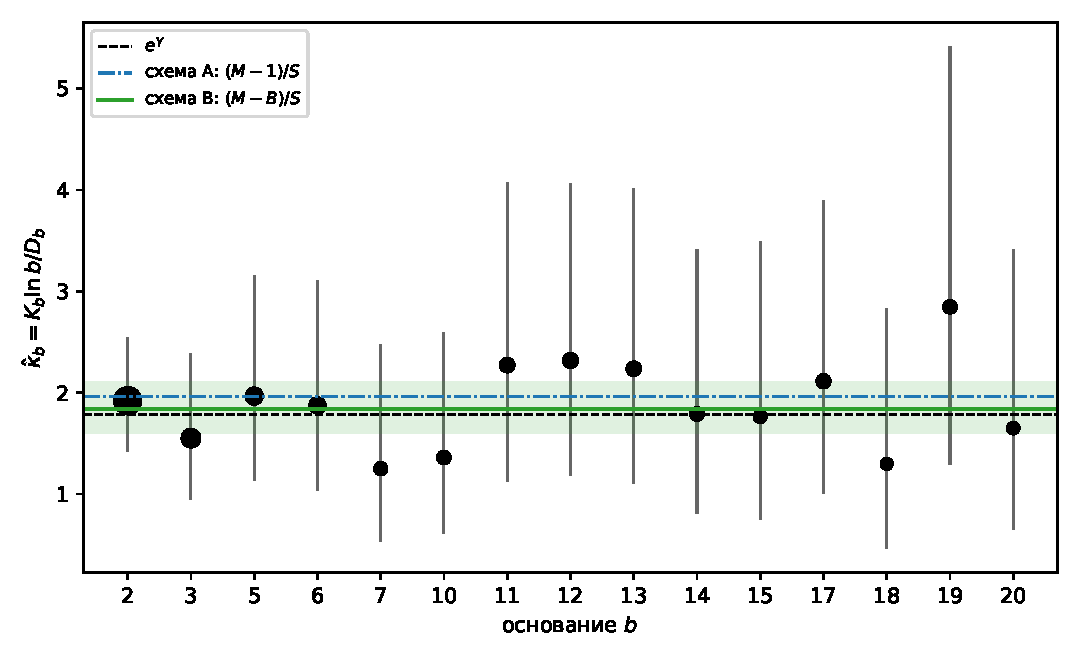
\includegraphics[width=.85\textwidth]{fig_kappa.pdf}
\caption{Оценки $\hat\kappa_b$ по основаниям с точными $95\%$ интервалами
Гарвуда~\eqref{eq:garwood}; площадь маркера пропорциональна $N_b$. Штриховая линия ---
значение ЛПВ $\eg$; зелёная с полосой --- объединённая оценка схемы~B и её
интервал; синяя штрихпунктирная --- оценка схемы~A $(M-1)/S$. Каждое основание по
отдельности совместимо с универсальной константой.
\encapfig{Per-base estimates $\hat\kappa_b$ with exact $95\%$ Garwood
intervals~\eqref{eq:garwood}; marker area is proportional to $N_b$. Dashed line: the
LPW value $\eg$; green with a band: the pooled scheme~B estimate and its interval;
blue dash-dotted: the scheme~A estimate $(M-1)/S$. Each base separately is
compatible with a universal constant.}}
\label{fig:kappa}
\end{figure}

\subsection{Однородность и её мощность}\label{sec:homog}

Пусть $H_0$ --- модель с единой $\kappa$, а $H_1$ --- модель со свободными $\kappa_b$.
Из условного правдоподобия предложения~\ref{prop:cond}, поскольку
$\sum_b\hat\kappa_bD_b/\ln b=K=\hat\kappa_{\mathrm B}S$, статистика
отношения правдоподобий сводится к
\begin{equation}\label{eq:LR}
\Lambda=2\sum_b K_b \ln\frac{\hat\kappa_b}{\hat\kappa_{\mathrm B}}
=2\sum_b K_b\ln\frac{K_b}{K\,s_b/S},\qquad s_b=\frac{D_b}{\ln b}.
\end{equation}
Существенно, что её нулевое распределение здесь \emph{точно}: обусловливание на
$K=\sum_bK_b$ превращает~\eqref{eq:pivotB} в мультиномиальную модель
$(K_b)\mid K\sim\mathrm{Multinomial}(K;\,s_b/S)$, и апеллировать к асимптотике
$\chi^2_{B-1}$ не нужно. Мы получаем $\Lambda=7{,}127$, точное $p=0{,}935$
($2\cdot10^6$ мультиномиальных реализаций, $\pm0{,}0003$ на уровне $95\%$); асимптотическое
приближение даёт $p=0{,}930$ при $14$ степенях свободы, то есть в данном случае
работает хорошо. Точный нулевой закон есть и при схеме~A: там при $H_0$ величины
$\kappa s_b$ независимы и распределены как $\Gam(N_b,1)$, так что вектор $s_b/S$
распределён по закону Дирихле с параметрами $N_b$ и от $\kappa$ не зависит; аналог
статистики~\eqref{eq:LR} с $N_b$ вместо $K_b$ равен $\Lambda_{\mathrm A}=7{,}395$
при точном $p=0{,}923$ ($\chi^2$: $0{,}918$; тег~[S30]).

Однако неотвержение информативно ровно настолько, насколько мощен критерий, и здесь
следует применить к себе то же требование, что и к литературе. Мы симулировали
альтернативы, в которых $\kappa_b$ логнормально рассеяны со средним $\eg$ и
коэффициентом вариации $cv$ (то есть $\ln\kappa_b$ имеет дисперсию $\ln(1+cv^2)$),
условно на наблюдённом $K$: $(K_b)\mid K\sim\mathrm{Multinomial}\bigl(K;\,
\kappa_bs_b/\sum_{b'}\kappa_{b'}s_{b'}\bigr)$; критическое значение --- $95\%$-квантиль
точного нулевого закона:

\begin{center}
\small
\begin{tabular}{lrrrrrrrrr}
\toprule
$cv$ & 0{,}05 & 0{,}10 & 0{,}15 & 0{,}20 & 0{,}25 & 0{,}30 & 0{,}35 & 0{,}40 & 0{,}50\\
мощность & 0{,}059 & 0{,}097 & 0{,}184 & 0{,}326 & 0{,}484 & 0{,}645 & 0{,}774 & 0{,}851 & 0{,}948\\
\bottomrule
\end{tabular}
\end{center}

Мощности $80\%$ критерий достигает лишь при $cv\approx0{,}37$ ($12\,000$ реализаций
на точку сетки, точность по мощности около $\pm0{,}004$). Центр распределения
$\kappa_b$ (среднее или медиана) на мощность не влияет: мультиномиальные
вероятности $\kappa_bs_b/\sum_{b'}\kappa_{b'}s_{b'}$ не меняются при умножении всех
$\kappa_b$ на одно число, и важен лишь разброс. Следовательно,
$p=0{,}935$ означает: данные не требуют базозависимых частот, но и не исключают
разброса $\kappa_b$ с коэффициентом вариации вплоть до трети. Утверждение
<<удачливых оснований не существует>> из имеющихся данных не следует; следует более
слабое --- <<их существование данными не поддерживается, а разброс с коэффициентом
вариации меньше $0{,}37$ обнаруживается с вероятностью ниже $80\%$>>.

\subsection{Устойчивость}\label{sec:robust}

\paragraph{Нижнее усечение.} Мы варьировали нижнюю точку усечения, чтобы прощупать
асимптотический режим (эвристика~\eqref{eq:LPW} асимптотична, тогда как модель
постоянной интенсивности стартует от $n=2$). Результаты в таблице~\ref{tab:trunc}.
Оценка схемы~A растёт с $1{,}965$ до $2{,}085$ в строго согласованном варианте
$N_b\ge1$ (до $2{,}099$ при отборе $N_b\ge2$) --- не строго монотонно (при
$n>10^{2}$ она отступает с $2{,}019$ до $2{,}012$), но систематически: рост
составляет $6{,}1\%$ ($6{,}8\%$) при том, что все значения получены на вложенных
подвыборках одних и тех же данных. Значимым трендом это, однако, не является: если
смоделировать данные на тех же началах отсчёта и числах событий (при схеме~B ---
с фронтом $W_b=N_b/\lambda_b$, правило <<$\mathbb E[\#]$ = наблюдённое>>
таблицы~\ref{tab:calib}), рост оценки схемы~A не меньше чем на $6{,}1\%$
встречается с вероятностью $0{,}219$ при схеме~A и $0{,}615$ при схеме~B (при отборе
$N_b\ge2$ для роста на $6{,}8\%$ --- $0{,}196$ и $0{,}597$; теги~[S29], [S30]). Оценка схемы~B восходящего
тренда не показывает и остаётся вблизи $\eg$, в пределах $1{,}757$--$1{,}871$ в строго согласованном
варианте $N_b\ge1$ (при отборе $N_b\ge2$ --- $1{,}789$--$1{,}871$), а её
$p$-значения на всех уровнях усечения лежат между $0{,}53$ и $1{,}00$. Причина видна
из~\eqref{eq:pivotB}: усечение уменьшает $M$, но не $B$, тогда как схема~A
вычитает единицу независимо от объёма выборки; разность двух оценок равна
$(B-1)/S$ и механически растёт, поскольку $S$ при усечении падает примерно со
$110$ до~$42$. Профиль усечения поэтому согласуется с диагнозом~\S\ref{sec:scheme}
и слабо свидетельствует в пользу схемы~B (отношение вероятностей около трёх), но
независимым подтверждением его не является. Начиная с $n>10$ оценка схемы~B
убывает ($1{,}871\to1{,}757$, на $6{,}1\%$, в строго согласованном варианте; до
$1{,}789$ при отборе $N_b\ge2$); и это в пределах шума вложенных подвыборок: при
схеме~B с тем же фронтом снижение от $n>10$ до $n>10^4$ не меньше наблюдённого
встречается с вероятностью $0{,}229$, а снижение от полной выборки до $n>10^4$ не
меньше наблюдённого ($4{,}4\%$) --- с вероятностью $0{,}306$ (при отборе $N_b\ge2$
для снижения на $2{,}7\%$ --- $0{,}308$; теги~[S29], [S30]). Член второго порядка это убывание не снимает
(\S\ref{sec:second}). Кривые приведены на рис.~\ref{fig:trunc}.

Результат не зависит и от того, где ставить начало отсчёта. Если помещать его в
саму точку усечения (тогда первое уцелевшее событие не теряется), оценка схемы~B
равна $1{,}891$, $1{,}867$, $1{,}906$ и $1{,}891$ при $n>10$, $10^2$, $10^3$, $10^4$
($p=0{,}43$--$0{,}60$). Если у пяти оснований с арифметически заданным началом
$n_{\min}=2$ (\S\ref{sec:bases}) перенести его на второй индекс, то
$(M-B)/S=1{,}882$ при $p=0{,}457$ (тег~[S29]).

\begin{table}[t]
\centering
\caption{Устойчивость к нижнему усечению. Основание остаётся в выборке, если после
усечения у него сохраняется не менее \emph{двух} событий ($N_b\ge2$); при $n>10^4$ этому
критерию перестаёт удовлетворять основание~19, откуда $B=14$. Критерий существен:
при более слабом требовании $N_b\ge1$ основание~19 сохраняется, что даёт последнюю
строку таблицы; строго согласована с предложением~\ref{prop:cond} именно она, так как
отбор по $N_b\ge2$ есть отбор по $K_b\ge1$ и смещает оценку вверх
(замечание~\ref{rem:selection}). Интервал и $p_{\mathrm B}$ --- точные, схемы~B;
последний столбец ($p_{\mathrm A}$, гамма-пивот схемы~A) приведён для сравнения
со старой практикой.
\encaptab{Robustness to lower truncation. A base is retained if at least
\emph{two} events survive the truncation ($N_b\ge2$); at $n>10^4$ base~19 no longer
meets this criterion, whence $B=14$. The criterion matters: under the weaker
requirement $N_b\ge1$ base~19 is retained, giving the last row; only that row is
strictly consistent with Proposition~\ref{prop:cond}, since selecting on $N_b\ge2$
means selecting on $K_b\ge1$ and biases the estimate upwards
(Remark~\ref{rem:selection}). The interval and $p_{\mathrm B}$ are exact, scheme~B; the last column ($p_{\mathrm A}$, the scheme~A
Gamma pivot) is given for comparison with the old practice.}}
\label{tab:trunc}
\small
\begin{tabular}{lrrrrlrr}
\toprule
усечение & $B$ & $M$ & $(M-1)/S$ & $(M-B)/S$ & 95\% ДИ, схема B
& $p_{\mathrm B}$ & $p_{\mathrm A}$\\
\midrule
нет & 15 & 218 & 1{,}9648 & 1{,}8381 & [1{,}594; 2{,}109] & 0{,}672 & 0{,}142\\
$n>10$ & 15 & 192 & 2{,}0192 & 1{,}8712 & [1{,}606; 2{,}168] & 0{,}531 & 0{,}080\\
$n>10^2$ & 15 & 156 & 2{,}0116 & 1{,}8299 & [1{,}540; 2{,}158] & 0{,}771 & 0{,}124\\
$n>10^3$ & 15 & 125 & 2{,}0551 & 1{,}8231 & [1{,}498; 2{,}197] & 0{,}832 & 0{,}106\\
$n>10^4$ & 14 & 89 & 2{,}0990 & 1{,}7889 & [1{,}407; 2{,}242] & 1{,}000 & 0{,}116\\
\midrule
$n>10^4$, $N_b\ge1$ & 15 & 90 & 2{,}0848 & 1{,}7569 & [1{,}382; 2{,}202] & 0{,}966 & 0{,}128\\
\bottomrule
\end{tabular}
\end{table}

\begin{figure}[t]
\centering
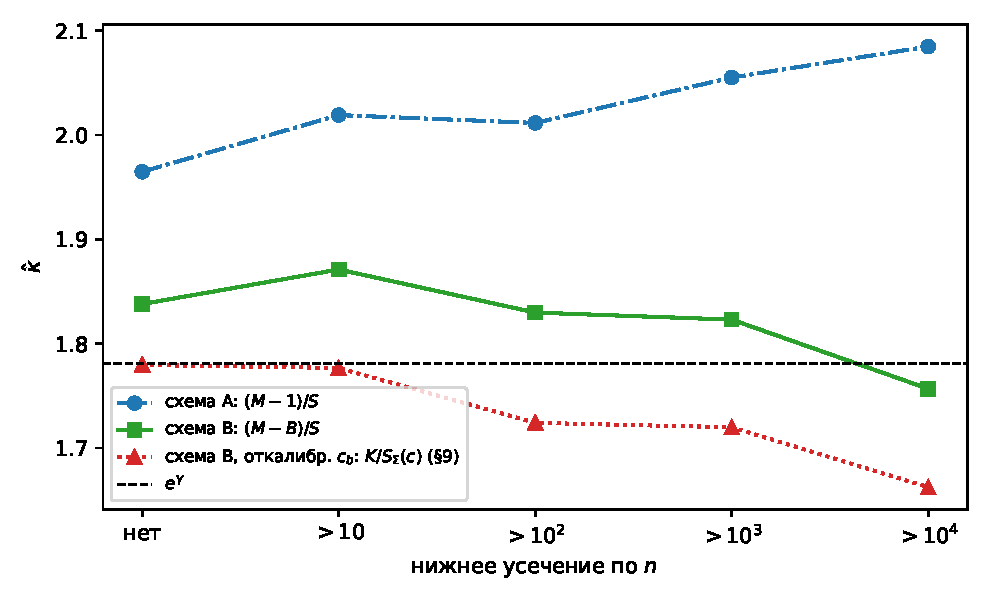
\includegraphics[width=.75\textwidth]{fig_truncation.pdf}
\caption{Объединённая оценка при нижнем усечении: $(M-1)/S$ (схема~A), $(M-B)/S$
(схема~B) и $K/S_\Sigma(c)$ с откалиброванным членом второго порядка и
экспозицией, суммированной по простым (\S\ref{sec:second}). Последняя точка
($n>10^4$) --- строго согласованный вариант $N_b\ge1$ (таблица~\ref{tab:trunc}).
Восходящий тренд схемы~A при переходе к схеме~B исчезает. Все кривые получены на вложенных
подвыборках, и их изменения при усечении лежат в пределах шума
(\S\ref{sec:robust}).
\encapfig{The pooled estimate under lower truncation: $(M-1)/S$ (scheme~A),
$(M-B)/S$ (scheme~B) and $K/S_\Sigma(c)$ with the measured second-order term and
the exposure summed over the primes (\S\ref{sec:second}). The last point
($n>10^4$) is the strictly consistent variant $N_b\ge1$ (Table~\ref{tab:trunc}).
The upward trend of scheme~A disappears under scheme~B. All curves come from nested subsamples, and
their changes under truncation are within the noise (\S\ref{sec:robust}).}}
\label{fig:trunc}
\end{figure}

\paragraph{Исключение по одному основанию.} Анализ с исключением одного основания даёт
$\hat\kappa_{\mathrm B}$ в пределах $[1{,}808;\,1{,}878]$ (крайние значения --- при
исключении $b=19$ и $b=3$) и точные $p$-значения в пределах $[0{,}49;\,0{,}85]$;
ни одно основание не определяет вывод.

\paragraph{Статус данных.} Ограничение основания~2 пятьюдесятью дважды проверенными
показателями переводит оценку схемы~B с $1{,}838$ на $1{,}834$ (схема~A: с
$\tilde\kappa=1{,}965$, $p=0{,}142$ на $\tilde\kappa=1{,}961$, $p=0{,}151$).
Статус PRP у большинства членов начинается гораздо ниже миллиона
(\S\ref{sec:data}), так что следующий вариант проверяет не PRP-статус как таковой, а
самые недавние и наименее перепроверенные находки: исключение всех индексов
$n>10^6$ даёт $M=182$ и $(M-B)/S=1{,}800$ ($\tilde\kappa=1{,}951$). В наихудшем
сценарии, когда последний известный PRP какого-либо основания оказывается составным,
наибольший сдвиг даёт $b=17$: $(M-B)/S=1{,}848$ ($\tilde\kappa=1{,}977$). Все
варианты лежат внутри как интервала~\eqref{eq:resA}, так и
интервала~\eqref{eq:resB}, поэтому возможные псевдопростые на вывод не влияют.
Существеннее не ложные находки, а пропущенные (\S\ref{sec:data}): пропуск занижает
$K$ при неизменном $S$ и смещает оценку вниз, в сторону основного вывода. Чтобы ЛПВ
отверглась сверху, внутри окон должно быть пропущено не меньше $23$ находок, по
$1{,}5$ на основание, а с членом второго порядка --- не меньше $30$ (тег~[S30]).
Две находки основания~5 2024~г. в окна не входят: они лежат выше $n_{\max}$, за
непройденным промежутком (\S\ref{sec:data}).

\section{Статистическая мощность}\label{sec:power}

Согласно~\eqref{eq:pivotB} мощность против истинной константы $\kappa=r\eg$ на уровне
$\alpha$ доступна в замкнутой форме (таблица~\ref{tab:power}). Конвенцию необходимо
оговаривать: всюду в этой работе критерий \emph{двусторонний}, с конвенцией
удвоенного минимального хвоста, $\alpha=0{,}05$. Односторонний вариант того же
критерия даёт заметно другие числа, и они приведены в правой части таблицы для
сопоставимости с работами, где конвенция не указана.

\begin{table}[t]
\centering
\caption{Мощность на уровне $\alpha=0{,}05$ для отвержения $\kappa=\eg$, когда истинная
константа превышает его в указанное число раз. Экспозиции: $S_2=26{,}02$ ($K=50$)
для одного основания~2 и $S=110{,}44$ ($K=203$) для объединения.
\encaptab{Power at level $\alpha=0.05$ for rejecting $\kappa=\eg$ when the true
constant exceeds it by the stated factor. Exposures: $S_2=26.02$ ($K=50$) for base~2
alone and $S=110.44$ ($K=203$) for the pooled sample.}}
\label{tab:power}
\small
\begin{tabular}{lrr@{\qquad}rr}
\toprule
& \multicolumn{2}{c}{двусторонний} & \multicolumn{2}{c}{односторонний}\\
\cmidrule(r){2-3}\cmidrule(l){4-5}
$\kappa/\eg$ & только Мерсенн & объединение & только Мерсенн & объединение\\
\midrule
1{,}05 & 0{,}060 & 0{,}099 & 0{,}082 & 0{,}165\\
1{,}10 & 0{,}099 & 0{,}266 & 0{,}147 & 0{,}386\\
1{,}15 & 0{,}164 & 0{,}514 & 0{,}235 & 0{,}644\\
1{,}20 & 0{,}253 & 0{,}752 & 0{,}343 & 0{,}844\\
1{,}30 & 0{,}479 & 0{,}972 & 0{,}581 & 0{,}988\\
1{,}50 & 0{,}861 & 1{,}000 & 0{,}910 & 1{,}000\\
\bottomrule
\end{tabular}
\end{table}

При мощности $80\%$ одна последовательность Мерсенна обнаруживает только отклонения
в $45{,}5\%$ и более; объединение пятнадцати оснований снижает этот порог до $21{,}3\%$
(односторонний вариант --- до $18{,}7\%$). Таблица~\ref{tab:power} относится к
превышению; для занижения константы пороги того же двустороннего критерия иные:
$37{,}4\%$ для одного основания~2 и $19{,}2\%$ для объединения (тег~[S29]).
Достижение мощности $80\%$ против отклонения в $10\%$ требует экспозиции
$S\approx470$, то есть $K\approx837$ условных событий ($M\approx852$) при
$\kappa=\eg$ (при истинной константе, на $10\%$ большей, ожидается $K\approx921$
условных событий, то есть $M\approx936$ находок);
против $5\%$ --- $S\approx1823$ и $K\approx3246$. Функция мощности дискретного
критерия немонотонна по $S$ (пилообразна), поэтому приведены значения, начиная
с которых мощность уже не опускается ниже $80\%$ (найдены сплошным просмотром по
$S$ с шагом $0{,}01$).

Эти рубежи вычислительно недостижимы, и стоит сказать насколько. Поскольку $K$ растёт
логарифмически по фронту поиска, удвоение фронтов \emph{по всем пятнадцати основаниям}
добавляет к экспозиции $\ln2\sum_b1/\ln b=5{,}41$, то есть в среднем
$\eg\cdot5{,}41=9{,}64$ условного события. Чтобы довести экспозицию с $110{,}4$ до
$470$, нужно $(470-110{,}4)/5{,}41\approx66{,}4$ удвоения, то есть рост фронтов
примерно в $2^{66{,}4}\approx10^{20}$ раз; для чувствительности в $5\%$ --- около
$316$ удвоений, то есть множитель порядка $10^{95}$. Речь идёт
не о десятилетиях, а о величинах, лежащих вне досягаемости любых мыслимых вычислений.
Обе кривые мощности как функции истинного отклонения показаны на
рис.~\ref{fig:power}.

\begin{figure}[t]
\centering
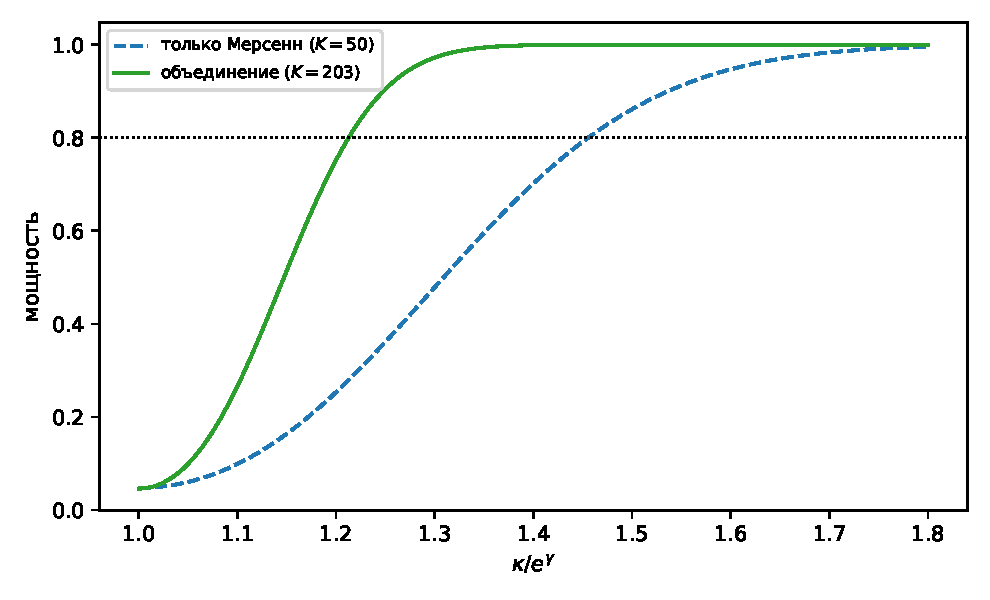
\includegraphics[width=.72\textwidth]{fig_power.pdf}
\caption{Мощность двустороннего отвержения $\kappa=\eg$ на уровне $\alpha=0{,}05$.
Горизонтальная линия отмечает мощность $80\%$.
\encapfig{Power of the two-sided rejection of $\kappa=\eg$ at level $\alpha=0.05$.
The horizontal line marks $80\%$ power.}}
\label{fig:power}
\end{figure}

Отсюда правило чтения для этой литературы. Сообщение о том, что данные согласуются с ЛПВ
с точностью до нескольких процентов, не есть свидетельство в пользу ЛПВ на уровне
нескольких процентов; оно совместимо с константой, ошибочной в полтора раза.
Объединённый анализ устанавливает, однако, настоящую границу: универсальная константа,
если она существует, при (A1) лежит примерно в $[1{,}59;\,2{,}11]$ в модели постоянной
интенсивности и в $[1{,}52;\,2{,}06]$ с откалиброванным членом второго порядка при $n>10$
(\S\ref{sec:second}); ни одно основание от неё различимо не отклоняется.

\section{Та же ошибка в ином обличье}\label{sec:sameerror}

Счётная функция Мерсенна провоцирует родственную ошибку, которую мы приводим как
разобранный пример. Регрессия $\pi_2(t)$ на~$t$ в точках событий по $50$ дважды
проверенным показателям (нумерация $0,\dots,N-1$: наименьший показатель есть начало
отсчёта, а не событие) даёт наклон $2{,}6391$ и свободный член $-2{,}9627$ при
стандартной ошибке МНК $0{,}4469$, на вид значимый и наводящий на мысль о вторичном
члене в~\eqref{eq:LPW}. Ничего подобного.

Складываются два дефекта. Остатки кумулятивного счёта сильно автокоррелированы,
здесь $\rho_1=0{,}825$ (выборочная корреляция соседних остатков; оценка
автокорреляционной функции даёт $0{,}751$); оценка Ньюи --- Уэста с ядром Бартлетта
и восемью лагами, без поправки на число степеней свободы, увеличивает стандартную
ошибку до $0{,}7315$ (с поправкой $n/(n-k)$ --- до $0{,}7466$; тег~[S30]). Существеннее то, что регрессия использует
только точки событий и тем самым отбрасывает пустой интервал между последним показателем
и фронтом поиска. Корректная нулевая модель удерживает интервал $[t_0,T]$ фиксированным,
где $T=\ln X_{\mathrm{ver}}$, и обусловливается ровно $N-1=49$ событиями строго правее
$t_0$, что по свойству порядковых статистик пуассоновского процесса при
заданном числе событий (ср.\ доказательство предложения~\ref{prop:unbiased}(b))
означает $49$ независимых равномерных точек на $(t_0,T]$. По $60\,000$ таким реализациям свободный член имеет медиану $-1{,}529$ и
$5$--$95\%$ диапазон $[-5{,}99;\,2{,}20]$, что даёт двусторонний $p=0{,}570$ для
наблюдённого значения. Вторичный член есть артефакт обусловливания. Заметим, что и
корректное нулевое распределение центрировано не в нуле. Счёт обращается в нуль в
$t_0=\ln2$, а свободный член измеряется в $t=0$, и одно это сдвигает его
примерно на $-\hat\lambda\ln2$, то есть почти на $-1{,}9$. Сравнивать $-2{,}96$ с
нулём неверно вдвойне: и из-за заниженной стандартной ошибки, и потому, что
нулевое ожидание не равно нулю.

\subsection{Три следствия одного и того же обусловливания}

\paragraph{(i) Бутстрэп не спасает.} Естественная реакция на подозрительно малую
стандартную ошибку МНК --- непараметрический бутстрэп пар по точкам событий. На
данных основания~2
бутстрэп по $20\,000$ ресемплам даёт медиану $-2{,}948$, стандартное отклонение
$0{,}385$ и $95\%$ интервал $[-3{,}809;\,-2{,}300]$, целиком лежащий ниже нуля; доля
отрицательных значений равна $100\%$. Это не подтверждение, а повторение той же ошибки:
ресемплинг наблюдённых точек воспроизводит изменчивость внутри реализованной
конфигурации и не может восстановить изменчивость самого процесса, породившего эту
конфигурацию. Корректное нулевое распределение имеет стандартное отклонение $2{,}499$
(в $5{,}6$ раза больше стандартной ошибки МНК $0{,}447$),
то есть в $6{,}5$ раза шире бутстрэпного \emph{по стандартному отклонению}
(по ширине $95\%$-интервала --- также в $6{,}5$ раза).

\paragraph{(ii) Мнимая недодисперсия.} Сравнение наблюдённого $\max_i|r_i|=6{,}347$,
где $r_i=i-\hat\lambda(t_i-t_0)$, с симуляцией \emph{необусловленного} пуассоновского
процесса наводит на вывод, что счётная функция <<глаже пуассоновской>>. Против
корректного нулевого распределения --- с обусловливанием на $N-1$ событий и оценкой
$\lambda$ по последнему из них --- медиана равна $5{,}117$, а двусторонний уровень
значимости составляет $0{,}529$. Наблюдение совершенно рядовое. Супремум без
нормировки нечувствителен вблизи закреплённых концов. Поэтому мы проверили и
вариант, стандартизованный по дисперсии моста,
$\max_i|r_i|/\sqrt{(N-1)u_i(1-u_i)}$ с $u_i=(t_i-t_0)/(t_{N-1}-t_0)$ по внутренним
событиям, при том же нулевом законе: он даёт $3{,}45$ при $p=0{,}194$, тоже рядовое
значение (тег~[S29]).

\paragraph{(iii) <<Серединный дефицит>>.} Оценивание $\lambda$ по последнему событию
обращает остаток $r$ в нуль на обоих концах ($r(t_0)=r(t_N)=0$ при правильной
нумерации), превращая его траекторию в аналог броуновского моста. Закрепление
концов определяет типичную величину экскурсии в середине диапазона, но не её знак:
мост асимптотически симметричен (при $N-1=49$ асимметрия пренебрежима), и
отрицательная экскурсия не менее вероятна, чем положительная такой же величины.
Наблюдённое среднее остатков $r_i$ в событиях средней половины оси~$t$, то есть с
$u_i\in[1/4,3/4]$, равно $-3{,}13$ при медиане симуляций
$-0{,}012$ и $p=0{,}272$; доля реализаций с отрицательной средней экскурсией
составляет $0{,}502$, то есть систематического дефицита нет. Сама траектория
остаточного процесса вместе с полосой симуляций приведена на
рис.~\ref{fig:bridge}.

\begin{figure}[t]
\centering
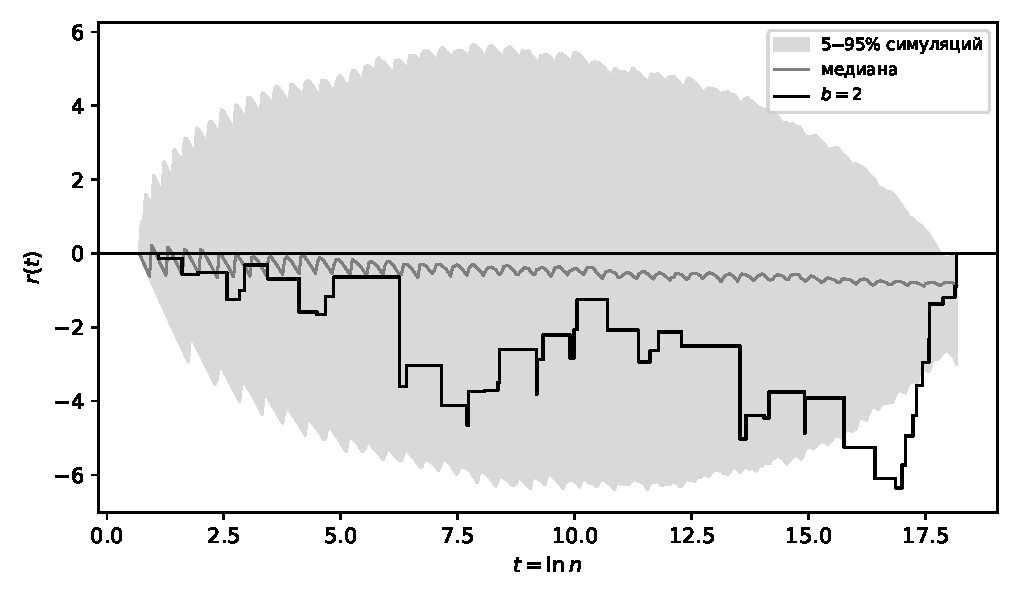
\includegraphics[width=.78\textwidth]{fig_resid_bridge.pdf}
\caption{Остаточный процесс $r(t)$ для основания $b=2$ вместе с поточечной полосой
$5$--$95\%$ квантилей и медианой симуляций. Полоса построена для той же ступенчатой
функции $r(t)=\#\{t_i\le t\}-\hat\lambda(t-t_0)$ при нулевом законе
\S\ref{sec:sameerror}: $49$ равномерных точек на $(t_0,\ln X_{\mathrm{ver}}]$,
$\hat\lambda$ по последней из них. Траектория выходит за полосу вблизи
$t\approx16{,}9$, где $r=-6{,}35$ при поточечном $5\%$-квантиле $-3{,}85$ (полоса
рисунка; независимая симуляция~[S29] даёт $-3{,}81$).
Поточечный выход о значимости не говорит: для всей траектории стандартизованный
супремум даёт $p=0{,}194$, обычный --- $p=0{,}529$ (\S\ref{sec:sameerror}, тег~[S29]).
\encapfig{The residual process $r(t)$ for base $b=2$ together with the pointwise
$5$--$95\%$ quantile band and the median of the simulations. The band is built for
the same step function $r(t)=\#\{t_i\le t\}-\hat\lambda(t-t_0)$ under the null law of
\S\ref{sec:sameerror}: $49$ uniform points on $(t_0,\ln X_{\mathrm{ver}}]$,
$\hat\lambda$ from the last of them. The trajectory leaves the band near
$t\approx16.9$, where $r=-6.35$ against a pointwise $5\%$ quantile of $-3.85$ (the
band drawn; an independent simulation~[S29] gives $-3.81$). A
pointwise exit says nothing about significance: for the whole trajectory the
standardized supremum gives $p=0.194$, the plain one $p=0.529$
(\S\ref{sec:sameerror}, tag~[S29]).}}
\label{fig:bridge}
\end{figure}

\subsection{Основание 2 на известном фронте}

Основание~2 --- одно из двух оснований основного набора с опубликованным фронтом
(второе --- $b=10$, \S\ref{sec:frontiers}); для него возможен анализ по схеме~B
\emph{с использованием полной экспозиции}, а не только условной. С
$T=\ln X_{\mathrm{ver}}$ получаем
$\hat\lambda=(N-1)/(T-t_0)=2{,}7960$ против $\eg/\ln2=2{,}5695$, то есть
$\hat\kappa_2=1{,}9381$ при точном $95\%$ интервале Гарвуда $[1{,}434;\,2{,}562]$ и
пуассоновском $p=0{,}593$ (удвоенный хвост; при mid-$p$-конвенции $0{,}545$ ---
конвенцию здесь необходимо оговаривать, поскольку различие ощутимо).
Условная оценка \emph{того же среза данных} --- те же $50$ дважды проверенных
показателей --- даёт $1{,}9046$; различие невелико, поскольку последний показатель
этого среза $77\,232\,917$ случайно оказался очень близко к фронту $81\,648\,221$.
(Для сравнения, условная оценка по всем $52$ известным показателям, приведённая в
таблице~\ref{tab:bases}, равна $1{,}9215$; сопоставлять её с $\hat\kappa_2$ нельзя ---
это другая выборка.) Это совпадение одной реализации, а не свойство метода:
поправка~\S\ref{sec:cost} относится к среднему по положению последнего события
относительно фронта.

Отметим попутно, что описанный здесь режим --- ровно тот, к которому мы призываем
перейти для всех оснований: при известном $W_b$ условное обусловливание на $D_b$
становится ненужным, и точность растёт на те самые $3{,}7\%$ из \S\ref{sec:exact}.

\subsection{Знак свободного члена ничего не доказывает}

В предыдущей редакции здесь приводился <<независимый довод>>: будто теоретический
вторичный член, $(\eg/\ln2)\mathfrak M=+0{,}672$ с постоянной Мейсселя ---
Мертенса $\mathfrak M=0{,}26150\ldots$, имеет знак, противоположный наблюдаемому
$-2{,}963$. Этот довод неверен, и мы его отзываем: в нём учтена лишь одна из двух
теорем Мертенса. Суммирование~\eqref{eq:probp} по простым $p\le x$ с
$\sum_{p\le x}\ln p/p=\ln x+E+o(1)$, $E=-1{,}3326\ldots$, и
$\sum_{p\le x}1/p=\ln\ln x+\mathfrak M+o(1)$ даёт
\[
\pi_2(x)\approx\frac{\eg}{\ln2}\bigl(\ln x+c_2\ln\ln x\bigr)+C_0,\qquad
C_0=\frac{\eg}{\ln2}\bigl(E+c_2\mathfrak M\bigr).
\]
При откалиброванном $c_2=0{,}96$ (\S\ref{sec:second}) получаем $C_0=-2{,}78$; прямое
суммирование по $p\le10^8$ даёт то же значение. Сама постоянная $C_0$ сильно
зависит от обращения с малыми $p$, где вероятность~\eqref{eq:probp} превышает
единицу: если ограничить вероятности единицей, получится $C_0=-5{,}05$ (тег~[S30]).
Свободный член регрессии --- тем более не $C_0$: он зависит ещё от нумерации
событий, от линеаризации члена $c_2\ln\ln x$ и от обусловливания на числе событий.
Надёжнее прямая проверка. Породим показатели Мерсенна самой
эвристикой --- испытаниями Бернулли по простым $p\le X_{\mathrm{ver}}$ с
вероятностью~\eqref{eq:probp} при откалиброванном $c_2$ --- и обусловим на $50$
событиях. Тогда свободный член той же регрессии имеет медиану $-2{,}52$ и
$5$--$95\%$ диапазон $[-5{,}20;\,-0{,}15]$, а наблюдённое $-2{,}963$ лежит на его
квантиле $0{,}385$; с уточнением Вагстаффа ($a=2$ или $6$) медиана равна $-2{,}32$,
квантиль --- $0{,}343$ (тег~[S28]). Эвристика второго порядка предсказывает
отрицательный свободный член той же величины, что и наблюдаемый. О структуре
свидетельствует не знак $C_1$, а лишь корректное нулевое распределение
(\S\ref{sec:sameerror}, $p=0{,}57$): свободный член $C_1$ --- параметр
аппроксимации, и содержательной трактовки не требует.

\section{Структурные поправки}\label{sec:struct}

Рассмотрим более общую параметризацию интенсивности $\lambda_b=(\kappa/\ln b)\,C_b$
и четыре модели множителя:
\begin{align*}
\text{I:}&\quad C_b=1;\\
\text{II:}&\quad C_b=\prod_{p\mid b-1,\ p\ne2}\Bigl(\tfrac{p}{p-1}\Bigr)^{\alpha}
                 \prod_{p\mid b+1,\ p\ne2}\Bigl(\tfrac{p}{p-2}\Bigr)^{\beta};\\
\text{III:}&\quad C_b=\prod_{p\mid b^2-1}\Bigl(\tfrac{p}{p-1}\Bigr)^{\eta};\\
\text{IV:}&\quad C_b=\exp\bigl(\theta_1\omega(b-1)+\theta_2\omega(b+1)+\theta_3\ln b\bigr).
\end{align*}
Модели занумерованы римскими цифрами, чтобы не смешивать их со схемами наблюдения~A
и~B; показатель в модели~III обозначен через $\eta$, чтобы не смешивать его с
постоянной Эйлера и с расстоянием до фронта $\delta_b$. Правдоподобие здесь --- \emph{условное пуассоновское}
предложения~\ref{prop:cond},
$\ell_{\mathrm B}=\sum_b\bigl[K_b\ln\mu_b-\mu_b-\ln K_b!\bigr]$ с
$\mu_b=\kappa C_b D_b/\ln b$; в предыдущей редакции использовалось
правдоподобие~\eqref{eq:loglik} схемы~A, что несовместимо с
\S\ref{sec:scheme}. Результаты в таблице~\ref{tab:struct}. Ни одна параметризация не
даёт значимого улучшения; байесовские факторы по BIC при $n=K=203$ сильно
поддерживают базовую модель против моделей~II и~IV ($112$ и $1112$) и умеренно ---
против~III ($10{,}6$; при $n=15$ --- $2{,}9$; тег~[S30]).

Модели~II--IV формализуют фольклорное представление об <<удачливых>> основаниях
через делители $b\pm1$, по образцу особого ряда Харди --- Литтлвуда. Теория такого
множителя не предсказывает: при нечётном простом $p\nmid b-1$ простые $q\mid b-1$
и $q\mid b+1$ не делят $\Rb(p)$, поскольку $\Rb(p)\equiv p$ и $\Rb(p)\equiv1\pmod q$ соответственно, но так
же ведут себя все простые $q<2p+1$ при любом~$b$ (\S\ref{sec:data}), и этот
выигрыш уже входит в общий множитель $\eg\ln(2p)$. Эвристика предсказывает
$C_b\equiv1$, так что этот параграф проверяет фольклор, а не теорию; содержательная
зависимость от основания второго порядка разобрана в~\S\ref{sec:second}.

\begin{table}[t]
\centering
\caption{Сравнение структурных моделей под условным пуассоновским правдоподобием
предложения~\ref{prop:cond} (полная форма, с $-\ln K_b!$); LR и $p$ даны относительно
модели~I; BIC вычислен при $n=K=203$.
\encaptab{Comparison of structural models under the conditional Poisson likelihood of
Proposition~\ref{prop:cond} (full form, including $-\ln K_b!$); LR and $p$ are
relative to model~I; BIC is computed with $n=K=203$.}}
\label{tab:struct}
\small
\begin{tabular}{lrrrrrrr}
\toprule
Модель & параметров & $\ln L$ & LR & $p$ & AIC & BIC & $P(\text{модель}\mid\text{данные})$\\
\midrule
I & 1 & $-35{,}753$ & --- & --- & 73{,}51 & 76{,}82 & 0{,}906\\
II & 3 & $-35{,}162$ & 1{,}18 & 0{,}554 & 76{,}32 & 86{,}26 & 0{,}008\\
III & 2 & $-35{,}458$ & 0{,}59 & 0{,}443 & 74{,}92 & 81{,}54 & 0{,}085\\
IV & 4 & $-34{,}797$ & 1{,}91 & 0{,}591 & 77{,}59 & 90{,}85 & 0{,}001\\
\bottomrule
\end{tabular}
\end{table}

\begin{remark}[Чувствительность BIC]
Выбор эффективного объёма выборки для BIC неочевиден: правдоподобие имеет
$B=15$ независимых слагаемых, но информация растёт как $K=203$. При $n=15$
апостериорные вероятности составляют $0{,}661$ / $0{,}080$ / $0{,}229$ / $0{,}030$,
при $n=203$ --- $0{,}906$ / $0{,}008$ / $0{,}085$ / $0{,}001$. Вывод в пользу модели~I
при обоих выборах, но при $n=203$ он существенно сильнее. Мы отчитываемся по
$n=K$ как соответствующему числу независимых условных событий.
\end{remark}

\paragraph{Фиксированная арифметическая поправка.} Отдельно рассмотрена модель с
\emph{фиксированным} (не оцениваемым) множителем
$C^{\mathrm{fix}}_b=\prod_{p\mid b-1,p\ne2}\frac{p}{p-1}\prod_{p\mid b+1,p\ne2}\frac{p}{p-2}$,
среднее значение которого по пятнадцати основаниям равно $2{,}462$. Она даёт
$\hat\kappa=0{,}759$. Подчеркнём, что сравнивать это значение с $\eg$ бессмысленно:
в перепараметризованной модели $\kappa$ имеет иной масштаб, и такой <<критерий
согласия>> проверял бы лишь равенство среднего $C_b$ единице. Поскольку модели~I и
$C^{\mathrm{fix}}$ ненестированы и имеют одинаковое число свободных параметров,
корректное сравнение --- прямо по правдоподобию: $\ln L=-51{,}53$ против $-35{,}75$,
разность $-15{,}78$. Фиксированная поправка решительно отвергается.

\paragraph{Логарифмические поправки.} Здесь необходимо исправление по существу.
Модель $\lambda_b(t)=(\kappa/\ln b)(1+c_1/t+c_2/t^2)$, использованная в предыдущей
редакции, \emph{не является допустимой интенсивностью}: при полученных там оценках
$\hat c_1=+0{,}108$, $\hat c_2=-0{,}826$ множитель обращается в нуль при
$t=0{,}8564$ и отрицателен левее, то есть при $n<2{,}355$; в частности, при
$t_0=\ln 2$ он равен $-0{,}5634$. Основания с $n_{\min}=2$ ($b=2,6,10,12,18$)
интегрируют интенсивность по области, где она отрицательна, и мера
$\int\lambda\,dt$ на этом участке отрицательна. То, что правдоподобие всё же
вычислялось, --- случайность: наименьший индекс, являющийся событием, равен $3$,
то есть $t=1{,}0986>0{,}8564$, так что под логарифм отрицательные значения не
попали.

Правильная параметризация того же семейства ---
\begin{equation}\label{eq:logcorr}
\lambda_b(t)=\frac{\kappa}{\ln b}\exp\Bigl(\frac{c_1}{t}+\frac{c_2}{t^2}\Bigr),
\end{equation}
положительная тождественно и вкладывающаяся в нулевую модель при $c_1=c_2=0$.
Она оценивается условным правдоподобием точечного
процесса~\eqref{eq:condinhom}: сумма $\sum\ln\lambda(t_i)$ берётся по событиям
\emph{без последнего}, а интеграл $\int\lambda$ --- от $t_0$ до последнего события
$t_0+D_b$, а не до неизвестного фронта (замечание~\ref{rem:inhom}; правдоподобие
одного лишь счёта здесь недопустимо: оно отбрасывает положения событий, которыми
только и определяются $c_1,c_2$). Результат: $\hat\kappa=1{,}748$,
$\hat c_1=0{,}75$, $\hat c_2=-1{,}44$; отношение правдоподобий против $c_1=c_2=0$
равно $2{,}03$ при двух степенях свободы, $p=0{,}36$ (тег~[S17]). Поскольку
$\hat c_1$ и $\hat c_2$ сильно коррелированы, асимптотика $\chi^2_2$ здесь не
гарантирована, и мы откалибровали её параметрическим бутстрэпом условной модели:
$p=0{,}366$ по $10\,000$ реализациям, $95\%$-квантиль $5{,}93$ против $5{,}99$ у
$\chi^2_2$ (тег~[S30]). Значимого улучшения нет. Оценка $\hat c_1$ здесь сильно коррелирована с $\hat c_2$ и сама по себе не
информативна: однопараметрическая модель~\eqref{eq:lam2} на тех же данных даёт
$\hat c=-0{,}40$ в интегральной форме и $1{,}03$ с экспозицией, суммированной по
простым (\S\ref{sec:second}).

\section{Член второго порядка самой эвристики}\label{sec:second}

До сих пор проверялась модель постоянной интенсивности~\eqref{eq:lam}. Но сама
эвристика ЛПВ предсказывает интенсивность, \emph{не} постоянную при конечных~$n$,
и это меняет смысл сравнения $\hat\kappa$ с $\eg$.

\paragraph{Вывод.} Пусть $p$ --- нечётное простое, $p\nmid b-1$, и $q$ --- простой делитель
$\Rb(p)$. Тогда $b$ имеет порядок $p$ по модулю $q$, откуда $q\equiv1\pmod p$, а
так как $\Rb(p)$ нечётно, $q\equiv1\pmod{2p}$. Значит, у $\Rb(p)$ нет простых
делителей меньше $2p+1$, и по теореме Мертенса вероятность простоты
увеличивается в $\prod_{q<2p}(1-1/q)^{-1}\approx\eg\ln(2p)$ раз по сравнению со
случайным числом той же величины. Это и есть вывод~\cite{wagstaff1983,t5k}:
\begin{equation}\label{eq:probp}
\Pr\bigl(\Rb(p)\ \text{простое}\bigr)\approx\frac{\eg\ln(a_bp)}{p\ln b}.
\end{equation}
Уточнение Вагстаффа для $b=2$ учитывает, что $q\equiv\pm1\pmod8$, и даёт $a=2$ при
$p\equiv3\pmod4$ и $a=6$ при $p\equiv1\pmod4$. В непрерывном приближении,
умножая~\eqref{eq:probp} на плотность простых $1/\ln n$ и переходя к $t=\ln n$,
получаем
\begin{equation}\label{eq:lam2}
\lambda_b(t)=\frac{\kappa}{\ln b}\Bigl(1+\frac{c_b}{t}\Bigr),\qquad
c_b=\langle\ln a_b\rangle,\qquad \kappa=\eg,
\end{equation}
а для счётной функции --- $\pi_b(x)\approx(\eg/\ln b)\,(\ln x+c_b\ln\ln x)$.
Асимптотика~\eqref{eq:LPW} от этого не меняется, но при $t\approx10$--$18$ поправка
$c_b/t$ составляет несколько процентов --- столько же, сколько обсуждаемые в работе
эффекты.

\paragraph{Калибровка $c_b$.} Приём Вагстаффа --- заменить $a_b$ наименьшим
допустимым кандидатом в делители --- груб, и мы оцениваем $c_b$ по фактической
делимости $\Rb(p)$ в рамках той же эвристики Мертенса. Для случайного числа $N$
по Мертенсу
\[
\Pr(N\ \text{простое}\mid\text{нет простых делителей}<Y)\approx\eg\ln Y/\ln N.
\]
Поэтому $\Pr(\Rb(p)\ \text{простое})\approx F_b(p,Y)\,\eg\ln Y/(p\ln b)$, где
$F_b(p,Y)$ --- индикатор того, что у $\Rb(p)$ нет простых делителей меньше $Y$.
Сравнение с~\eqref{eq:probp} даёт
\begin{equation}\label{eq:cbemp}
c_b(Y)=\bigl\langle F_b(p,Y)\ln Y-\ln p\bigr\rangle_p .
\end{equation}
Индикатор $F_b$ вычисляется \emph{точно}. При $p>b$ простой делитель $\Rb(p)$
меньше $Y$ существует тогда и только тогда, когда $b^p\equiv1\pmod q$ для
некоторого $q=2kp+1<Y$, простого или нет. Действительно, простые делители такого
$q$, не делящие $b-1$, сравнимы с $1$ по модулю $p$ и делят $\Rb(p)$; часть $q$,
составленная из делителей $b-1$, по лемме о подъёме показателя делит $b-1<p$ и
сравнима с $1\pmod p$, поэтому равна~$1$. Для $31\,598$ простых
$p\in[2\cdot10^4,\,4\cdot10^5)$ и $Y=100p$, $1000p$, $3000p$ получаем значения
$c_b$, устойчивые по $Y$ в пределах стандартной ошибки $0{,}05$ (скрипт
\texttt{cb\_empirical.py}, тег~[S19]; значения при разных $Y$ получены на одном и
том же наборе $p$ и потому коррелированы). При $Y=1000p$ они лежат от $0{,}43$
($b=12$) до $1{,}11$ ($b=20$), в среднем $0{,}67$. У десяти оснований из пятнадцати
оценка $c_b$ \emph{ниже} $\ln2\approx0{,}693$ --- значения, которое даёт наивное
применение теоремы Мертенса к одному условию $q\equiv1\pmod{2p}$; следовательно,
$\ln2$ не является нижней границей эффективного $c_b$. Приём Вагстаффа
(усреднение $\ln a_b$ с учётом того, что $b$ --- квадратичный вычет по
модулю~$q$) даёт систематически большие значения, от $1{,}23$ до $1{,}74$
(тег~[S14]); даже для $b=2$ он даёт $1{,}242=\tfrac12(\ln2+\ln6)$ против
$0{,}96\pm0{,}05$. К тому же этот приём неоднозначен: кандидаты, делящиеся на
простой делитель $b$, отбрасываются, а делящиеся на прочие малые простые --- нет;
так, при $b=18$ условие вычета совпадает с условием для $b=2$, но
$c_{18}=1{,}646$ против $c_2=1{,}242$. Ниже основной считается калибровка
$c_b$~\eqref{eq:cbemp}, а вариант Вагстаффа приводится лишь для сравнения.

\paragraph{Откуда берутся значения $c_b$.} Калибровку можно предсказать, не
вычисляя $b^p\bmod q$ (скрипт \texttt{cb\_theory.py}, тег~[S23]). Простое
$q=2kp+1$ делит $\Rb(p)$ тогда и только тогда, когда $b$ лежит в подгруппе
индекса $2k$ группы $\mathbb F_q^{*}$. Для этого необходимо, чтобы $b$ был
квадратичным вычетом по модулю~$q$, а это детерминировано символом Якоби
$(b/q)$. Внутри подгруппы вычетов естественная эвристика --- равномерность, и она
даёт вероятность $2/(2k)=1/k$; при $k=1$ это $1$, что и есть классический случай
$2p+1\mid M_p$ при $p\equiv3\pmod4$. Отсюда прогноз
\begin{equation}\label{eq:cbth}
F^{\mathrm{th}}_b(p,Y)=\prod_{\substack{k<Y/(2p):\ q=2kp+1\ \text{простое},\\ (b/q)=+1}}
\Bigl(1-\frac1k\Bigr),\qquad
c^{\mathrm{th}}_b=\bigl\langle F^{\mathrm{th}}_b(p,Y)\ln Y-\ln p\bigr\rangle_p ,
\end{equation}
использующий лишь простоту чисел $2kp+1$ и квадратичный характер~$b$.
Таблица~\ref{tab:cbth} сравнивает его с калибровкой на тех же $31\,598$ простых
$p$. Корреляция равна $0{,}976$, средняя разность $+0{,}017$. Парный критерий по
каждому~$p$ даёт $\sum z_b^2=23{,}5$ при $15$ степенях свободы, $p=0{,}074$. Прогноз
объясняет $95\%$ разброса $c_b$ между основаниями. Наибольшее отклонение ---
у $b=2$ ($+0{,}12$, $z=2{,}6$); его естественный источник --- не учтённый моделью
биквадратичный характер двойки (критерий Гаусса). Из~\eqref{eq:cbth} следует и
структурный вывод: в этом приближении $c_b$ зависит лишь от бесквадратной части
$b$. Пары $2$ и $18$, $3$ и $12$, $5$ и $20$ имеют одинаковый прогноз, и
калибровка подтверждает это в пределах погрешности. Тем самым значения $c_b$ ---
и то, что приём Вагстаффа их завышает, --- объясняются распределением простых
вида $2kp+1$ и квадратичным законом взаимности, а не особенностями данных.

\begin{table}[t]
\centering
\caption{Член второго порядка $c_b$: калибровка по фактической делимости
(формула~\eqref{eq:cbemp}, тег~[S19]) и прогноз~\eqref{eq:cbth} по простоте $2kp+1$ и
символу $(b/q)$ (тег~[S23]); $z$ --- парная $z$-статистика разности; $31\,598$
простых $p\in[2\cdot10^4,\,4\cdot10^5)$, $Y=1000p$.
\encaptab{The second-order term $c_b$: calibration from the actual divisibility
(equation~\eqref{eq:cbemp}, tag~[S19]) and the prediction~\eqref{eq:cbth} from the primality
of $2kp+1$ and the symbol $(b/q)$ (tag~[S23]); $z$ is the paired $z$-statistic of
the difference; $31\,598$ primes $p\in[2\cdot10^4,\,4\cdot10^5)$, $Y=1000p$.}}
\label{tab:cbth}
\small
\setlength{\tabcolsep}{2.6pt}
\begin{tabular}{lrrrrrrrrrrrrrrr}
\toprule
$b$ & 2 & 3 & 5 & 6 & 7 & 10 & 11 & 12 & 13 & 14 & 15 & 17 & 18 & 19 & 20\\
\midrule
калибровка & 0{,}96 & 0{,}44 & 1{,}06 & 0{,}59 & 0{,}49 & 0{,}55 & 0{,}47 & 0{,}43 & 0{,}67 & 0{,}53 & 0{,}54 & 0{,}76 & 0{,}86 & 0{,}54 & 1{,}11\\
прогноз & 0{,}84 & 0{,}46 & 1{,}01 & 0{,}50 & 0{,}51 & 0{,}52 & 0{,}53 & 0{,}46 & 0{,}75 & 0{,}51 & 0{,}52 & 0{,}71 & 0{,}84 & 0{,}54 & 1{,}01\\
$z$ & $+2{,}6$ & $-0{,}4$ & $+1{,}1$ & $+2{,}0$ & $-0{,}5$ & $+0{,}7$ & $-1{,}3$ & $-0{,}8$ & $-1{,}8$ & $+0{,}4$ & $+0{,}3$ & $+1{,}0$ & $+0{,}4$ & $-0{,}1$ & $+2{,}0$\\
\bottomrule
\end{tabular}
\end{table}

\paragraph{Условный вывод при заданном $c$.} По
замечанию~\ref{rem:inhom} условно на $D_b$ внутренние события образуют
пуассоновский процесс с той же интенсивностью на $(t_0,t_0+D_b)$. Но
эвристика~\eqref{eq:probp} задаёт вероятность не на оси~$t$, а для каждого простого
индекса, и ожидаемое число событий в окне есть \emph{сумма по простым}. Поэтому
предложение~\ref{prop:cond} переносится в виде
\begin{equation}\label{eq:pivotc}
K\mid(D_b)_b\sim\Pois\bigl(\kappa S_\Sigma(c)\bigr),\qquad
S_\Sigma(c)=\sum_b\frac{1}{\ln b}\sum_{\substack{n_{\min}<p<n_{\max}\\ p\ \text{простое}}}
\frac{\ln p+c_b}{p},
\end{equation}
где из внутренней суммы исключены детерминированно составные случаи $p\mid b-1$ и
$p=s$ (Орифейль, \S\ref{sec:bases}). Оценка есть $K/S_\Sigma(c)$, и интервал
Гарвуда~\eqref{eq:garwood} применим с заменой $S$ на $S_\Sigma(c)$. Пуассоновский
закон~\eqref{eq:pivotc} точен для пуассоновского процесса с
интенсивностью~\eqref{eq:lam2}. Если же понимать эвристику буквально, как испытания
Бернулли на простых индексах с вероятностями~\eqref{eq:probp}, ограниченными
единицей, то обусловливание на последней находке остаётся корректным (испытания до
неё от этого события не зависят), но условный закон $K$ становится
пуассон-биномиальным: $\operatorname{Var}(K\mid D)/\mathbb E[K\mid D]=0{,}934$ на
полной выборке и $0{,}973$ при $n>10$ (тег~[S30]). Пуассоновские интервалы и
$p$-значения поэтому консервативны: стандартное отклонение завышено на $3{,}5\%$ и
$1{,}4\%$. Грубый учёт общей для оснований простоты чисел $2p+1$ возвращает
отношение дисперсии к среднему почти к единице (замечание~\ref{rem:indep}).
Непрерывное приближение~\eqref{eq:lam2} заменяет эту сумму интегралом:
\begin{equation}\label{eq:pivotcint}
S(c)=\sum_b\frac{D_b+c_b\ln\bigl((t_0+D_b)/t_0\bigr)}{\ln b}.
\end{equation}
Оно точно лишь асимптотически. По первой теореме Мертенса
$\sum_{p\le x}\ln p/p=\ln x+E+o(1)$ с $E=-1{,}3326\ldots$, и при началах отсчёта
$n_{\min}=2$--$19$ интеграл завышает экспозицию основания на $0{,}39$--$1{,}42$ по
$t$, в среднем на $1{,}04$; при нижнем усечении $n>10^2$ различие меньше
процента (тег~[S26]). В предыдущей редакции использовалась
форма~\eqref{eq:pivotcint}, и на полной выборке и при $n>10$ она занижала оценку
на $9{,}0\%$ и $3{,}8\%$ соответственно; ниже основной считается
форма~\eqref{eq:pivotc}.

\begin{table}[t]
\centering
\caption{Условный вывод с членом второго порядка: оценка $\hat\kappa$ и точное
двустороннее $p$ против $\kappa=\eg$. <<$c{=}0$>> --- модель постоянной
интенсивности; <<калибр., $\int$>> --- откалиброванные $c_b$ (тег~[S19]) с
интегральной экспозицией~\eqref{eq:pivotcint} прежней редакции; <<калибр.,
$\Sigma$>> --- те же $c_b$ с экспозицией~\eqref{eq:pivotc}, суммированной по
простым (основной вариант); <<В, $\Sigma$>> --- $c_b$ по приёму Вагстаффа с той же
суммой. Усечение, как в таблице~\ref{tab:trunc}. Теги~[S20], [S26].
\encaptab{Conditional inference with the second-order term: the estimate
$\hat\kappa$ and the exact two-sided $p$ against $\kappa=\eg$. ``$c{=}0$'' is the
constant-rate model; ``meas., $\int$'' are the measured $c_b$ (tag~[S19]) with the
integral exposure~\eqref{eq:pivotcint} of the previous version; ``meas., $\Sigma$''
are the same $c_b$ with the exposure~\eqref{eq:pivotc} summed over the primes (the
main variant); ``W, $\Sigma$'' is Wagstaff's device with the same sum. Truncation
as in Table~\ref{tab:trunc}. Tags~[S20], [S26].}}
\label{tab:second}
\small
\setlength{\tabcolsep}{4pt}
\begin{tabular}{lrrrrrrrr}
\toprule
& & \multicolumn{4}{c}{$\hat\kappa$} & \multicolumn{3}{c}{$p$}\\
\cmidrule(lr){3-6}\cmidrule(l){7-9}
усечение & $K$ & $c{=}0$ & калибр., $\int$ & калибр., $\Sigma$ & В, $\Sigma$
& $c{=}0$ & калибр., $\Sigma$ & В, $\Sigma$\\
\midrule
нет & 203 & 1{,}838 & 1{,}620 & 1{,}780 & 1{,}618 & 0{,}672 & 1{,}000 & 0{,}178\\
$n>10$ & 177 & 1{,}871 & 1{,}710 & 1{,}777 & 1{,}644 & 0{,}531 & 1{,}000 & 0{,}303\\
$n>10^2$ & 141 & 1{,}830 & 1{,}703 & 1{,}724 & 1{,}615 & 0{,}771 & 0{,}740 & 0{,}261\\
$n>10^3$ & 110 & 1{,}823 & 1{,}713 & 1{,}720 & 1{,}626 & 0{,}832 & 0{,}760 & 0{,}366\\
$n>10^4$ & 75 & 1{,}789 & 1{,}690 & 1{,}693 & 1{,}614 & 1{,}000 & 0{,}712 & 0{,}429\\
\midrule
$n>10^4$, $N_b\ge1$ & 75 & 1{,}757 & 1{,}660 & 1{,}663 & 1{,}585 & 0{,}966 & 0{,}598 & 0{,}340\\
\bottomrule
\end{tabular}
\end{table}

\paragraph{Результаты.} Таблица~\ref{tab:second} и модельная проверка дают пять
выводов.

\emph{(i) Внутри последовательностей член второго порядка определяется слабо, но
калибровке не противоречит.} Профильная ОМП общего $c$ по условному правдоподобию
с экспозицией~\eqref{eq:pivotc} на всех данных равна $1{,}03$ с $95\%$
интервалом $[-0{,}18;\,3{,}25]$: против $c=0$ получаем $p=0{,}111$, против $c=\ln2$
--- $p=0{,}654$. При $n>10$ оценка равна $0{,}82$, близко к среднему
откалиброванных $c_b$ ($0{,}67$), но интервал расширяется до $[-1{,}15;\,5{,}19]$, а при
$n>10^3$ информация практически исчезает (тег~[S26]): сдвиг $c$ компенсируется
сдвигом $\kappa$. Поэтому $c_b$ нужно брать извне --- из теории или, как здесь, из
калибровки~\eqref{eq:cbemp}. В предыдущей редакции та же профильная оценка по
интегральной форме~\eqref{eq:pivotcint} давала $-0{,}40$, и интервал
$[-0{,}69;\,0{,}44]$ исключал $c=\ln2$ ($p=0{,}017$, тег~[S15]). Это был артефакт
приближения: у нижнего конца окна интеграл завышает экспозицию, и подгонка
компенсировала это отрицательным~$c$.

\emph{(ii) Вывод о $\kappa$ от члена второго порядка зависит столь же сильно, как
от схемы наблюдения.} Переход от модели постоянной интенсивности к
откалиброванным $c_b$ снижает оценку на $3{,}2\%$ на полной выборке и на
$5{,}0$--$5{,}8\%$ при усечении (тег~[S26]). Это сравнимо с ценой выбора схемы
наблюдения ($6{,}9\%$, \S\ref{sec:cost}) и не меньше остаточного разрыва $(M-B)/S$
с $\eg$ ($3{,}2\%$ на полной выборке, $5{,}1\%$ при $n>10$). Сравнение оценки
модели постоянной интенсивности с $\eg$ --- не проверка ЛПВ при конечных $n$: сама
ЛПВ предсказывает, что такая оценка \emph{выше} $\eg$, на $3$--$8\%$ (см.~(v)).

\emph{(iii) ЛПВ со своим откалиброванным членом второго порядка согласуется с
данными.} При откалиброванных $c_b$ точное $p$ лежит в пределах
$0{,}598$--$1{,}000$ при любом уровне усечения. При завышенных значениях Вагстаффа
получается $0{,}26$--$0{,}43$ при $n>10$ и $0{,}178$ на полной выборке. Полная
выборка включает $n\le10$, где вероятность~\eqref{eq:probp} при малых $b$
превышает единицу (при $b=2$ --- при $p=3$, $5$ и $7$), а сами индексы $2,3,5,7$
продиктованы арифметикой малых чисел. Поэтому основным мы считаем вывод при
$n>10$; с суммой по простым он, впрочем, практически совпадает с выводом по полной
выборке ($1{,}777$ и $1{,}780$).

\emph{(iv) Убывание при усечении членом второго порядка не объясняется.} При $c=0$
оценка убывает с ростом нижней границы, с $1{,}871$ при $n>10$ до $1{,}757$ при
$n>10^4$ в строго согласованном варианте ($-6{,}1\%$; при отборе $N_b\ge2$ --- до
$1{,}789$, $-4{,}4\%$). В предыдущей редакции утверждалось, что это убывание
предсказано~\eqref{eq:lam2} и исчезает при его учёте: с интегральной
экспозицией~\eqref{eq:pivotcint} четыре оценки при $n>10$ лежали в пределах
$1{,}690$--$1{,}713$. Это утверждение мы отзываем: выравнивание создавалось той же
непрерывной аппроксимацией, которая сильнее всего завышает экспозицию у малых
$n_{\min}$. С суммой по простым оценки равны $1{,}777$, $1{,}724$, $1{,}720$ и
$1{,}693$ (в строго согласованной строке $N_b\ge1$ --- $1{,}663$) и от $n>10$ до
$n>10^4$ убывают на $6{,}4\%$ в строго согласованном варианте ($4{,}7\%$ при отборе
$N_b\ge2$) --- столько же, сколько при $c=0$. Если данные
порождены самой эвристикой, модель постоянной интенсивности завышает $\kappa$ почти
постоянно, на $5{,}7$--$8{,}3\%$ при $n>10$ (тег~[S27]), то есть убывания эвристика
не предсказывает. Само убывание в пределах шума вложенных подвыборок: при схеме~B
снижение не меньше наблюдённого встречается с вероятностью $0{,}229$
(\S\ref{sec:robust}).

\emph{(v) Погрешность $c_b$ и проверка метода на модельных данных.} Погрешность
калибровки ($\pm0{,}045$ по каждому основанию) на вывод практически не влияет:
её вклад в стандартное отклонение $\hat\kappa$ равен $0{,}003$--$0{,}004$ против
пуассоновских $0{,}12$. Совместный $95\%$ интервал с экспозицией~\eqref{eq:pivotc}
--- смесь интервалов Гарвуда по разбросу $c_b$: нижний конец решает уравнение
$\langle\Pr(\Gam(K,1)\le L\,S_\Sigma(c))\rangle_c=0{,}025$, верхний ---
$\langle\Pr(\Gam(K+1,1)\le U\,S_\Sigma(c))\rangle_c=0{,}975$ --- равен
$[1{,}543;\,2{,}042]$ на полной выборке и $[1{,}525;\,2{,}059]$ при $n>10$ и в третьем
знаке совпадает с интервалом Гарвуда при фиксированных $c_b$: погрешность
калибровки меняет экспозицию лишь на $0{,}21\%$ (тег~[S26]). В предыдущей редакции
приводился интервал джеффрисовского типа, $[1{,}546;\,2{,}036]$; он уже гарвудовского,
что для интервала, учитывающего дополнительную неопределённость, неверно. Прогноз $c^{\mathrm{th}}_b$ вместо калибровки даёт
$\hat\kappa=1{,}789$ и $1{,}784$ (тег~[S26]). Метод проверен на модельных данных,
порождённых самой эвристикой на уровне простых индексов (тег~[S27], $10\,000$
реализаций). Каждое простое $p>n_{\min}$ давало событие с
вероятностью~\eqref{eq:probp} при $\kappa=\eg$ и откалиброванных $c_b$; фронт
ставился на средний интервал дальше реальной последней находки, и к данным
применялся тот же анализ. Оценка $K/S_\Sigma(c)$ несмещена:
$\mathbb E[\hat\kappa]/\kappa=0{,}995$--$1{,}009$ при усечении до $n>10^3$, покрытие
интервала Гарвуда равно $0{,}955$--$0{,}961$. Интегральная форма~\eqref{eq:pivotcint}
на тех же данных занижает $\kappa$ на $9\%$ на полной выборке (покрытие $0{,}723$) и
на $3\%$ при $n>10$. Модель постоянной интенсивности завышает $\kappa$ на
$3$--$8\%$. При $n>10^4$ обе оценки с членом второго порядка смещаются вверх на
$2{,}4$--$2{,}5\%$; это отбор оснований по $N_b\ge2$, о котором предупреждает подпись
таблицы~\ref{tab:trunc}. Прежняя проверка (тег~[S25]) порождала данные из
непрерывной интенсивности~\eqref{eq:lam2} и потому не могла обнаружить погрешности
интегральной формы.

\paragraph{Следствие для фольклора.} Член $c_b\ln\ln x$ в счётной функции объясняет
и наблюдение, с которого начиналась работа: нормированные частоты лежат ниже
$\emg$ и медленно сходятся к нему снизу. В непрерывном
приближении~\eqref{eq:lam2} наклон $t_k$ по $k$ равен $\emg\ln b/(1+c_b\langle1/t\rangle)$, так что нормированная частота
занижена в $1+c_b\langle1/t\rangle$ раз, где
$\langle1/t\rangle=\ln(t_N/t_0)/(t_N-t_0)$. При фиксированном начале отсчёта это
убывает как $\ln t/t$, и частота стремится к $\emg$ как $\ln\ln n/\ln n$ --- ещё
медленнее, чем $1/\ln n$ (для $b=2$: $\langle1/t\rangle=0{,}183$ против
$1/t_N=0{,}053$). В~\S\ref{sec:notbias} показано, что
подгонка к правому концу эффекта не создаёт; здесь видно, откуда он берётся:
из самой эвристики, а не из~$\kappa\ne\eg$.

\paragraph{Итог.} Вопрос <<совместимы ли данные с ЛПВ>> распадается на два:
о главном члене, $\kappa=\eg$, и о члене второго порядка, $c_b$. Второй почти не
определяется положениями находок, но его можно откалибровать по фактической
делимости $\Rb(p)$~\eqref{eq:cbemp}. Ожидаемое число находок при этом нужно
суммировать по простым индексам: интеграл с плотностью $1/\ln n$ при малых $n$
завышает экспозицию на постоянную Мертенса. С откалиброванными $c_b$ оценка равна
$\hat\kappa\approx1{,}66$--$1{,}78$ при любом нижнем усечении (на $0{,}1$--$7\%$ ниже
$\eg$) с точным $p\ge0{,}598$: ЛПВ не отвергается. Убывание оценки при
усечении этим членом не снимается и лежит в пределах шума. Сами значения $c_b$
предсказываются из первых принципов --- по
простоте чисел $2kp+1$ и квадратичному характеру $b$~\eqref{eq:cbth} --- с
корреляцией $0{,}976$; метод проверен на модельных данных. Открытыми остаются
замкнутая формула для $c_b$ и поправка высших степенных характеров (заметная у
$b=2$).

\section{Заключение}

\begin{enumerate}
\item Употребительные оценки нормированной частоты обобщённых репьюнитных простых
\emph{не} смещены схемой подгонки: и концевая форма, и наклон МНК несмещены точно при
схеме~A и с экспоненциально малой по $\mu$ погрешностью при схеме~B (не более
$0{,}73\%$ для концевой формы и $2{,}3\%$ для МНК при $\mu\ge7$).
Смещена лишь обратная величина, и это следствие выпуклости. Расхожее объяснение
<<медленной сходимости снизу>> через цензурирование несостоятельно при обеих схемах;
настоящее её объяснение --- член второго порядка самой эвристики (п.~7).

\item Настоящий дефект употребительной практики --- в том, что различные формы оценки
расходятся до $29{,}5\%$, а точечные значения публикуются без доверительных интервалов
при том, что стандартные ошибки МНК в этой задаче занижены: поправка Ньюи ---
Уэста увеличивает их в $1{,}6$ раза, а корректное условное нулевое распределение
шире номинального в $5{,}6$ раза (\S\ref{sec:sameerror}).
Классификация оснований на <<удачливые>> и <<неудачливые>> переворачивается от смены
формы оценки на неизменных данных; у двух оснований из пятнадцати переворачивается
даже знак отклонения от $\emg$. Самое большое расхождение, у основания~18, создано
одним аномальным промежутком при арифметически заданном начале отсчёта.

\item Главный результат --- точное условное правдоподобие схемы~B. Незаписанные
фронты суть мешающие параметры Неймана --- Скотта, и профильная оценка $M/S$
несостоятельна. Положение последнего события $D_b$ достаточно для фронта, и
условно на нём величина $N_b-1$ распределена в пуассоновской модели как
$\Pois(\lambda_bD_b)$ при любом не зависящем от находок правиле выбора фронта;
условие относится к фактическому горизонту поиска, а опубликованная граница может
зависеть от находок (замечание~\ref{rem:weaker}). Тот же результат даёт
интегрирование по фронту с инвариантной мерой $dW_b$. Отсюда $M-B\mid D\sim\Pois(\kappa S)$:
правильным пивотом при фиксированном фронте является пуассоновский, а не
$\Gam(M,1)$, правильной объединённой оценкой --- $(M-B)/S$, а не $(M-1)/S$, и
доверительные интервалы получаются в замкнутой форме без симуляционной инверсии.
Условное правдоподобие стоит одного события на каждое основание, а не одного
события в сумме, --- точный аналог потери одной степени свободы на группу в
примере Неймана --- Скотта. Различение таких схем и сам аппарат восходят к теории
надёжности и к теории условного правдоподобия; новое здесь --- постановка с
недокументированным фронтом, когда экспозицию нельзя взять из протокола и её
приходится восстанавливать из находок (замечание~\ref{rem:priority}).

\item При (A1) это даёт $\hat\kappa=1{,}838$ при точном $95\%$ интервале
$[1{,}594;\,2{,}109]$ и $p=0{,}672$ против $\eg$. Сообщавшееся десятипроцентное
превышение над ЛПВ, включая наше собственное в более ранней редакции этой работы,
при (A1) создаётся в основном схемой наблюдения: переход к схеме~B сокращает его до
$3{,}2\%$, а остаток объясняется членом второго порядка самой эвристики (п.~7).
Старый гамма-пивот при схеме~B отвергает верную гипотезу в $11$--$17\%$ случаев.
Без (A1) неизвестное правило остановки входит через один параметр --- средний
зазор $m$ между последней находкой и фронтом, --- и ЛПВ не отвергается при любом $m$
от $0$ до $3{,}2$ (с членом второго порядка --- до $2{,}8$), то есть и при остановке
на находке, и при засухе $g=2$; от $m$ зависит лишь остаточное
превышение, $10{,}8\%$ при $m=0$ и нуль при $m=1{,}42$. Переход к схеме~B устраняет
восходящий тренд объединённой оценки при усечении по $n_{\min}$; и тренд, и
остающееся убывание ($1{,}871\to1{,}757$ от $n>10$ до $n>10^4$; при схеме~B снижение не меньше такого имеет вероятность $0{,}229$) лежат
в пределах шума вложенных подвыборок.

\item Помимо пуассоновской модели и сплошного покрытия поиска, вывод о схеме
наблюдения держится на допущении (A1): фронт выбирался без оглядки на находки. По
самим находкам его практически не проверить: $(M-1)/S$ и $(M-B)/S$ суть функции
одних и тех же статистик и различаются на $6{,}9\%$. Без (A1) строго сохраняется лишь верхняя
граница $M/S$ в смысле ожиданий (тождество Вальда); правило <<остановиться после
долгой полосы без находок>> смещает вверх и $(M-B)/S$, так что двусторонней вилки
нет, но превышения над ЛПВ такое нарушение не создаёт. Четыре документированных фронта
(A1) не решают: три из них старше снимка данных и дают лишь нижние границы зазора,
а синхронный фронт $b=2$ с (A1) согласуется. При отклонении в сторону остановки
вблизи находки верная оценка лежит, в смысле ожиданий, между $(M-B)/S$ и $M/S$, и
обе границы согласуются с ЛПВ; гибридная оценка с известным фронтом $b=2$ равна
$1{,}846$ ($1{,}853$ с добавлением $b=10$), а оценка по общему заведомо пройденному окну
$n\le2\cdot10^5$ --- $1{,}890$. Пропуски в поиске смещают оценку вниз; чтобы ЛПВ
отверглась сверху, их должно быть не меньше $23$. Практическое следствие --- необходимость публиковать фронты поиска $L_b$
(а вместе с ними и протоколы полноты просеивания), как это делает GIMPS для $b=2$.
Пример основания~$5$, где найденные в 2024~г. вероятно простые лежат за
непройденным промежутком, показывает, что это не формальность.

\item Гипотеза ЛПВ имеющимися данными не отвергается, а базозависимые поправки не
требуются. Но и то и другое --- утверждения о низкой чувствительности критериев:
условный мультиномиальный критерий однородности различает лишь разброс $\kappa_b$
с коэффициентом вариации порядка $0{,}37$, а объединённый критерий --- превышение
константы не менее чем на $21{,}3\%$ и занижение не менее чем на $19{,}2\%$
(двусторонний вариант). Достижение чувствительности в $10\%$ потребовало
бы роста фронтов поиска примерно в $10^{20}$ раз.

\item Сама эвристика ЛПВ предсказывает при конечных $n$ интенсивность
$(\kappa/\ln b)(1+c_b/t)$, и сравнение оценки модели постоянной интенсивности с
$\eg$ не является проверкой ЛПВ. Положения находок $c_b$ определяют слабо, но
его можно откалибровать по фактической делимости $\Rb(p)$: $c_b=0{,}43$--$1{,}11$,
в среднем $0{,}67$, тогда как приём Вагстаффа даёт вдвое большие значения.
Экспозицию при этом нужно суммировать по простым индексам: интеграл с плотностью
$1/\ln n$ при малых $n$ завышает её на постоянную Мертенса и занижал бы оценку на
$9{,}0\%$. С откалиброванным $c_b$ оценка при (A1) равна $1{,}66$--$1{,}78$ при
любом уровне усечения, ЛПВ не отвергается ($p\ge0{,}598$), а <<медленная сходимость
снизу>> получает объяснение; убывания оценки при усечении этот член не снимает.
Сами $c_b$ предсказываются по простоте чисел $2kp+1$ и квадратичному характеру $b$
(корреляция с калибровкой $0{,}976$) и зависят лишь от бесквадратной части $b$;
модельная проверка на данных, порождённых эвристикой на уровне простых индексов,
подтверждает несмещённость метода.
Открыты замкнутая формула для $c_b$ и поправка высших степенных характеров.
\end{enumerate}


\appendix
\section{Верификация исходных данных}\label{app:data}

Все двадцать последовательностей (пятнадцать основного набора и пять из проверки
границы отбора) сверены с записями OEIS 27 августа 2026~г.
Поскольку в объединённый анализ входят только тройки $(N_b,n_{\min},n_{\max})$,
в таблице~\ref{tab:verify} для основного набора приведены число известных простых, из которого
$N_b$ получается вычитанием единицы, и оба крайних индекса; полные списки
индексов содержатся в скрипте \texttt{analysis\_v2.py}.

\begin{table}[h]
\centering
\caption{Сверка с OEIS. Столбец <<последнее пополнение>> указывает происхождение
наибольшего известного индекса; для $b=2$ два последних показателя взяты у GIMPS.
\encaptab{Cross-check against OEIS. The column ``last addition'' gives the
provenance of the largest known index; for $b=2$ the last two exponents are taken
from GIMPS.}}
\label{tab:verify}
\small
\begin{tabular}{rlrrrl}
\toprule
$b$ & OEIS & простых & $n_{\min}$ & $n_{\max}$ & последнее пополнение\\
\midrule
2 & A000043 & 52 & 2 & 136\,279\,841 & GIMPS, окт.\ 2024\\
3 & A028491 & 23 & 3 & 8\,530\,117 & R.~Propper, 09.11.2023\\
5 & A004061 & 19 & 3 & 3\,300\,593 & R.~Propper, 02.01.2022\\
6 & A004062 & 17 & 2 & 3\,360\,347 & R.~Propper, 30.10.2023\\
7 & A004063 & 10 & 5 & 1\,264\,699 & P.~Bourdelais\\
10 & A004023 & 11 & 2 & 8\,177\,207 & Propper и Batalov, май 2021\\
11 & A005808 & 13 & 17 & 1\,868\,983 & P.~Bourdelais\\
12 & A004064 & 14 & 2 & 769\,543 & P.~Bourdelais, дек.\ 2014\\
13 & A016054 & 13 & 5 & 1\,503\,503 & P.~Bourdelais\\
14 & A006032 & 11 & 3 & 1\,724\,417 & P.~Bourdelais, 13.07.2026\\
15 & A006033 & 10 & 3 & 639\,833 & P.~Bourdelais, 22.04.2019\\
17 & A006034 & 12 & 3 & 1\,990\,523 & P.~Bourdelais, 03.08.2020\\
18 & A133857 & 8 & 2 & 1\,270\,141 & P.~Bourdelais\\
19 & A006035 & 11 & 19 & 209\,359 & P.~Bourdelais, 27.08.2010\\
20 & A127995 & 9 & 3 & 984\,349 & P.~Bourdelais\\
\bottomrule
\end{tabular}
\end{table}

Отдельно предупредим читателя, сверяющего данные по вторичным источникам: сводные
таблицы (страница <<Repunit primes>> в OEIS Wiki, статья <<List of repunit primes>>
в Википедии) обновляются с запаздыванием и на момент написания работы отставали
от самих записей OEIS на один член у оснований $b=14,15,17,18,20$. Авторитетным
источником следует считать записи OEIS.

\subsection*{Независимый пересчёт префиксов}

Сверка с OEIS подтверждает, что перечисленные индексы дают простое, но не
гарантирует \emph{полноты}: пропущенный член сдвинул бы $N_b$, а с ним и обе
объединённые оценки. Этот пробел мы закрыли прямым пересчётом. Для каждого из
двадцати оснований $2\le b\le26$, не являющихся точными степенями, независимой
реализацией\footnote{Гибридный CPU/GPU поисковик: сегментное сито по малым
делителям, trial factoring в арифметике Монтгомери, PRP через GMP и GWNUM/IBDWT.
Исходный код и протокол прогонов --- в том же репозитории, скрипты
\texttt{verify\_sequences.sh} и \texttt{compare\_verify.py}.} проверены
\emph{все} индексы $n<10^4$ подряд, а не только перечисленные в OEIS.
Отрицательные вердикты бывают двух видов: найденный делитель (сито и пробное
деление; это сертификат составности) и отрицательный тест Ферма. В окончательном
прогоне каждый вердикт второго вида пересчитан вторым, независимым бэкендом
(сплошной double-check, как в GIMPS), чтобы исключить потерянную находку.

Результат: $153$ члена подтверждены, лишних нет, пропущенных нет, расхождений
между бэкендами нет --- по всем двадцати основаниям. Покрытие по основаниям
неравномерно (от одного члена при $b=18$ до двадцати двух при $b=2$): на
основной набор $b\le20$ приходится $128$ подтверждённых индексов из $233$
известных. Выше $10^4$ полный пересчёт вычислительно недоступен, и там мы
по-прежнему опираемся на OEIS.

Отметим, что этот пересчёт не был формальностью. Первый прогон шёл с выборочным
двойным счётом ($5\%$ вердиктов, режим по умолчанию), и независимая реализация
объявила $R_{23}(3181)$ составным, разойдясь с A204940; расхождение обнаружила сверка
с OEIS, а не двойной счёт. Разбор показал ошибку в самой реализации --- всплеск
ошибки округления FFT на последней итерации, после последней периодической
проверки, --- а не в данных OEIS. После исправления (проверка ошибки округления
после цикла и досчёт на GMP при отказе GWNUM) пересчёт повторён со сплошным двойным
счётом, и расхождений не осталось. Мы приводим этот эпизод как иллюстрацию к тезису
\S\ref{sec:data} о полноте покрытия: одиночный отрицательный вердикт ненадёжен,
ложное <<составное>> невидимо без повторного счёта, и именно поэтому фронты и
протоколы проверки должны публиковаться.

\section*{Доступность данных и кода}
Все использованные последовательности приведены в таблице~\ref{tab:data}.

\emph{Данные.} Скрипт \texttt{fetch\_data.sh} загружает b-файлы OEIS для всех
пятнадцати последовательностей основного набора, \texttt{fetch\_extra.sh} --- для
пяти оснований $21\le b\le26$, использованных в проверке границы отбора
(\S\ref{sec:bases}). Загруженные файлы включены в репозиторий, так что анализ
воспроизводится без обращения к сети.

\emph{Анализ.} Каждое число настоящей работы помечено тегом вида~[S3],
соответствующим разделу или таблице, в выводе одного из скриптов
(\texttt{results\_v2.txt} или \texttt{results\_v3.txt}). Основной скрипт ---
\texttt{analysis\_v2.py} (numpy, scipy, matplotlib). Объединённый анализ, все
доверительные интервалы, критерий однородности, расчёты мощности и структурные
модели зависят только от троек $(N_b,n_{\min},n_{\max})$; полные списки индексов
нужны лишь для столбца $\hat G^{\mathrm{OLS}}_b$ таблицы~\ref{tab:bases}, для
\S\ref{sec:sameerror}, для усечения и для моделей с переменной интенсивностью.
Скрипт читает их из b-файлов каталога \texttt{data/} (загрузчик общий с
\texttt{analysis.py} версии~1). Генератор случайных чисел инициализирован
фиксированным зерном ($20260914$), поэтому все величины Монте-Карло воспроизводятся
побитово. Скрипт также строит все четыре рисунка (каталог \texttt{figs\_v2/},
английские подписи --- \texttt{figs\_v2/en/}). Таблицу~\ref{tab:stop}
(правила остановки, нарушающие (A1)) строит отдельный скрипт
\texttt{stopping\_rules.py} (тег~[S13], зерно $20260924$). Член второго
порядка (\S\ref{sec:second}), модель~\eqref{eq:logcorr} и критерий однородности при
$B=20$ вычисляет \texttt{lpw\_second\_order.py} (теги~[S14]--[S17], [S20]),
калибровку $c_b$ --- \texttt{cb\_empirical.py} (тег~[S19], детерминирован, около
десяти минут счёта), её теоретический прогноз --- \texttt{cb\_theory.py}
(тег~[S23]), учёт погрешности $c_b$ и модельную проверку метода ---
\texttt{sim\_second\_order.py} (теги~[S24], [S25]), проверку (A1) по
документированным фронтам и гибридную оценку --- \texttt{frontiers.py} (тег~[S18],
источники фронтов перечислены в самом скрипте). Экспозицию члена второго порядка,
суммированную по простым, профильную оценку общего $c$, модельную проверку с
генерацией на уровне простых индексов и симуляцию свободного члена
\S\ref{sec:sameerror} вычисляет \texttt{lpw\_prime\_sum.py} (теги~[S26]--[S28],
зерно $20260930$); дополнительные проверки устойчивости (значимость профиля
усечения, общий фронт $2\cdot10^5$, выбор начала отсчёта, основание~18, пороги
мощности для занижения, рис.~\ref{fig:bridge}) --- \texttt{robust\_extra.py}
(тег~[S29]); расчёты по решению редактора (семейство $(M-Bm)/S$, чувствительность к
пропускам, пуассон-биномиальный закон, ковариация оснований, отбор по числу
находок, бутстрэп для модели~\eqref{eq:logcorr} и др.) --- \texttt{revision\_v32.py}
(тег~[S30], зерно $20261001$). Вывод этих скриптов сохранён в
\texttt{results\_v3.txt}. Скрипты
\texttt{check\_numbers\_v3.py} и \texttt{check\_all\_numbers\_v3.py} сверяют с ним
все десятичные числа обеих версий статьи.

\emph{Независимый пересчёт последовательностей.} \texttt{verify\_sequences.sh}
запускает поисковик по всем индексам $n<10^4$ для каждого основания,
\texttt{compare\_verify.py} сверяет результат с b-файлами OEIS и возвращает
ненулевой код при любом расхождении (приложение~\ref{app:data}).

\emph{Оговорка о величинах Монте-Карло.} Основной результат~\eqref{eq:resB},
интервалы таблицы~\ref{tab:bases}, таблицы~\ref{tab:mfamily}, \ref{tab:trunc}
и~\ref{tab:power} \emph{детерминированы}: они получены точной инверсией
пуассоновского распределения и от генератора случайных чисел не зависят. От
симуляции зависят лишь таблицы~\ref{tab:mc}, \ref{tab:calib} и~\ref{tab:stop}, точное
$p$-значение критерия однородности и кривая его мощности, а также нулевые
распределения \S\ref{sec:sameerror}; их точность указана на месте. Это отличие от
предыдущей редакции существенно: там симуляционной была и сама основная оценка
интервала.

Репозиторий: \url{https://github.com/Wilps93/repunit-hunt} --- каталог
\texttt{paper/}. Дерево файлов и порядок запуска описаны в \texttt{paper/README.md}.

% п. 4.14 ГОСТ Р 7.0.7-2021: перечень затекстовых библиографических ссылок
% предваряют словами «Список источников»; babel-russian по умолчанию печатает
% «Список литературы», поэтому \refname переопределяем.
\renewcommand{\refname}{Список источников}
\begin{thebibliography}{99}

\bibitem{wagstaff1983} Wagstaff S.~S., Jr. Divisors of Mersenne numbers~//
Mathematics of Computation. 1983. Vol.~40, №~161. P.~385--397.
DOI: 10.1090/S0025-5718-1983-0679454-X.

\bibitem{pomerance1981} Pomerance C. Recent developments in primality testing~//
The Mathematical Intelligencer. 1981. Vol.~3, №~3. P.~97--105.
DOI: 10.1007/BF03022861.

\bibitem{t5k} Heuristics: deriving the Wagstaff Mersenne conjecture
[Электронный ресурс] // The PrimePages: prime number research and records.
URL: \url{https://t5k.org/mersenne/heuristic.html} (дата обращения: 27.08.2026).

\bibitem{dubner1993} Dubner H. Generalized repunit primes~//
Mathematics of Computation. 1993. Vol.~61, №~204. P.~927--930.
DOI: 10.1090/S0025-5718-1993-1185243-9.

\bibitem{bourdelais2009} Bourdelais P. A generalized repunit conjecture
[Электронный ресурс]~// NMBRTHRY mailing list. 25 June 2009.
URL: \url{https://listserv.nodak.edu/cgi-bin/wa.exe?A2=NMBRTHRY;417ab0d6.0906}
(дата обращения: 25.08.2026).

\bibitem{oeis} The On-Line Encyclopedia of Integer Sequences
[Электронный ресурс] / OEIS Foundation Inc.
URL: \url{https://oeis.org} (дата обращения: 27.08.2026).

\bibitem{wagstaff2025} Wagstaff S.~S., Jr. Two Mersenne prime conjectures
[Электронный ресурс]~// Journal of Integer Sequences. 2025. Vol.~28.
Article 25.7.2.
URL: \url{https://cs.uwaterloo.ca/journals/JIS/VOL28/Wagstaff/wag14.html}
(дата обращения: 24.09.2026).

\bibitem{dominguez2026} Dominguez J. Arithmetic bias in the distribution of Mersenne
prime exponents and the divisor structure of $p-1$ [Электронный ресурс] // arXiv.
2026. arXiv:2603.08994v6. URL: \url{https://arxiv.org/abs/2603.08994}
(дата обращения: 01.10.2026).

\bibitem{neymanscott1948} Neyman J., Scott E.~L. Consistent estimates based on
partially consistent observations~// Econometrica. 1948. Vol.~16, №~1. P.~1--32.
DOI: 10.2307/1914288.

\bibitem{andersen1970} Andersen E.~B. Asymptotic properties of conditional
maximum-likelihood estimators~// Journal of the Royal Statistical Society.
Series~B. 1970. Vol.~32, №~2. P.~283--301.
DOI: 10.1111/j.2517-6161.1970.tb00842.x.

\bibitem{gallagher1976} Gallagher P.~X. On the distribution of primes in short
intervals~// Mathematika. 1976. Vol.~23, №~1. P.~4--9.
DOI: 10.1112/S0025579300016442.

\bibitem{maier1985} Maier H. Primes in short intervals~// Michigan Mathematical
Journal. 1985. Vol.~32, №~2. P.~221--225. DOI: 10.1307/mmj/1029003189.

\bibitem{jha2026} Jha A. The Poisson tail conjecture for primes in short intervals
[Электронный ресурс] // arXiv. 2026. arXiv:2605.23014.
URL: \url{https://arxiv.org/abs/2605.23014} (дата обращения: 27.08.2026).

\bibitem{gimps} PrimeNet [Электронный ресурс] / Great Internet Mersenne Prime
Search (GIMPS). Программное обеспечение Prime95/MPrime, версия~30.8.
URL: \url{https://www.mersenne.org/} (дата обращения: 27.08.2026;
отчёт \emph{Milestones} считан 27.08.2026 04:30~UTC).

\bibitem{epstein1954trunc} Epstein B. Truncated life tests in the exponential
case~// The Annals of Mathematical Statistics. 1954. Vol.~25, №~3. P.~555--564.
DOI: 10.1214/aoms/1177728723.

\bibitem{epsteinsobel1954} Epstein B., Sobel M. Some theorems relevant to life
testing from an exponential distribution~// The Annals of Mathematical
Statistics. 1954. Vol.~25, №~2. P.~373--381. DOI: 10.1214/aoms/1177728793.

\bibitem{bartholomew1963} Bartholomew D.~J. The sampling distribution of an
estimate arising in life testing~// Technometrics. 1963. Vol.~5, №~3.
P.~361--374. DOI: 10.1080/00401706.1963.10490104.

\bibitem{sengupta2009} Sengupta S.~N., Sinha B.~K., Bagchi S.~B. Estimation of
mean life and reliability for exponential life distribution using time censored
sample data~// Statistics \& Probability Letters. 2009. Vol.~79, №~7.
P.~899--906. DOI: 10.1016/j.spl.2008.11.026.

\bibitem{kivela2015} Kivel\"{a} M., Porter M.~A. Estimating interevent time
distributions from finite observation periods in communication networks~//
Physical Review~E. 2015. Vol.~92, №~5. Article~052813.
DOI: 10.1103/PhysRevE.92.052813.

\bibitem{straussSadler1989} Strauss D., Sadler P.~M. Classical confidence
intervals and Bayesian probability estimates for ends of local taxon ranges~//
Mathematical Geology. 1989. Vol.~21, №~4. P.~411--427. DOI: 10.1007/BF00897326.

\bibitem{marshall1990} Marshall C.~R. Confidence intervals on stratigraphic
ranges~// Paleobiology. 1990. Vol.~16, №~1. P.~1--10.
DOI: 10.1017/S0094837300009672.

\bibitem{solow1993} Solow A.~R. Inferring extinction from sighting data~//
Ecology. 1993. Vol.~74, №~3. P.~962--964. DOI: 10.2307/1940821.

\bibitem{robsonwhitlock1964} Robson D.~S., Whitlock J.~H. Estimation of a
truncation point~// Biometrika. 1964. Vol.~51, №~1--2. P.~33--39.
DOI: 10.1093/biomet/51.1-2.33.

\bibitem{liu2023} Liu Z., Bhandaram U., Garg N. Quantifying spatial
under-reporting disparities in resident crowdsourcing~// Nature Computational
Science. 2024. Vol.~4, №~1. P.~57--65. DOI: 10.1038/s43588-023-00572-6.

\bibitem{lancaster2000} Lancaster T. The incidental parameter problem since
1948~// Journal of Econometrics. 2000. Vol.~95, №~2. P.~391--413.
DOI: 10.1016/S0304-4076(99)00044-5.

\bibitem{kalbfleischsprott1970} Kalbfleisch J.~D., Sprott D.~A. Application of
likelihood methods to models involving large numbers of parameters (with
discussion)~// Journal of the Royal Statistical Society. Series~B. 1970.
Vol.~32, №~2. P.~175--208. DOI: 10.1111/j.2517-6161.1970.tb00830.x.

\bibitem{berger1999} Berger J.~O., Liseo B., Wolpert R.~L. Integrated
likelihood methods for eliminating nuisance parameters~// Statistical Science.
1999. Vol.~14, №~1. P.~1--28. DOI: 10.1214/ss/1009211804.

\bibitem{lindsay1980} Lindsay B.~G. Nuisance parameters, mixture models, and
the efficiency of partial likelihood estimators~// Philosophical Transactions
of the Royal Society of London. Series~A. 1980. Vol.~296, №~1427. P.~639--662.
DOI: 10.1098/rsta.1980.0197.

\bibitem{repunithunt} Докучаев Т.~С. repunit-hunt: поиск обобщённых репьюнитных
простых и статистический анализ [Электронный ресурс]~// GitHub. 2026.
URL: \url{https://github.com/Wilps93/repunit-hunt} (дата обращения: 24.09.2026).

\bibitem{garwood1936} Garwood F. Fiducial limits for the Poisson distribution~//
Biometrika. 1936. Vol.~28, №~3--4. P.~437--442. DOI: 10.1093/biomet/28.3-4.437.

\end{thebibliography}

% ── Романизированный список для международных баз цитирования ──────────────
% Все использованные источники англоязычны, поэтому транслитерация не
% требуется: список воспроизводит те же записи в том же порядке.
\begin{otherlanguage}{english}
\section*{References}
\begin{enumerate}\itemsep2pt
\item Wagstaff S.~S., Jr. Divisors of Mersenne numbers.
\emph{Mathematics of Computation}, 1983, vol.~40, no.~161, pp.~385--397.
DOI: 10.1090/S0025-5718-1983-0679454-X

\item Pomerance C. Recent developments in primality testing.
\emph{The Mathematical Intelligencer}, 1981, vol.~3, no.~3, pp.~97--105.
DOI: 10.1007/BF03022861

\item Heuristics: deriving the Wagstaff Mersenne conjecture. \emph{The PrimePages:
prime number research and records}. Available at:
\url{https://t5k.org/mersenne/heuristic.html} (accessed 27.08.2026).

\item Dubner H. Generalized repunit primes.
\emph{Mathematics of Computation}, 1993, vol.~61, no.~204, pp.~927--930.
DOI: 10.1090/S0025-5718-1993-1185243-9

\item Bourdelais P. A generalized repunit conjecture. \emph{NMBRTHRY mailing
list}, 25 June 2009. Available at:
\url{https://listserv.nodak.edu/cgi-bin/wa.exe?A2=NMBRTHRY;417ab0d6.0906}
(accessed 25.08.2026).

\item OEIS Foundation Inc. \emph{The On-Line Encyclopedia of Integer
Sequences}. Available at: \url{https://oeis.org} (accessed 27.08.2026).

\item Wagstaff S.~S., Jr. Two Mersenne prime conjectures.
\emph{Journal of Integer Sequences}, 2025, vol.~28, article 25.7.2.
Available at:
\url{https://cs.uwaterloo.ca/journals/JIS/VOL28/Wagstaff/wag14.html}
(accessed 24.09.2026).

\item Dominguez J. Arithmetic bias in the distribution of Mersenne prime exponents
and the divisor structure of $p-1$. \emph{arXiv}, 2026, arXiv:2603.08994v6. Available
at: \url{https://arxiv.org/abs/2603.08994} (accessed 01.10.2026).

\item Neyman J., Scott E.~L. Consistent estimates based on partially consistent
observations. \emph{Econometrica}, 1948, vol.~16, no.~1, pp.~1--32.
DOI: 10.2307/1914288

\item Andersen E.~B. Asymptotic properties of conditional maximum-likelihood
estimators. \emph{Journal of the Royal Statistical Society. Series~B}, 1970,
vol.~32, no.~2, pp.~283--301. DOI: 10.1111/j.2517-6161.1970.tb00842.x

\item Gallagher P.~X. On the distribution of primes in short intervals.
\emph{Mathematika}, 1976, vol.~23, no.~1, pp.~4--9.
DOI: 10.1112/S0025579300016442

\item Maier H. Primes in short intervals. \emph{Michigan Mathematical Journal},
1985, vol.~32, no.~2, pp.~221--225. DOI: 10.1307/mmj/1029003189

\item Jha A. The Poisson tail conjecture for primes in short intervals.
\emph{arXiv}, 2026, arXiv:2605.23014. Available at:
\url{https://arxiv.org/abs/2605.23014} (accessed 27.08.2026).

\item Great Internet Mersenne Prime Search (GIMPS). \emph{PrimeNet}.
Prime95/MPrime software, version 30.8. Available at:
\url{https://www.mersenne.org/} (accessed 27.08.2026).

\item Epstein B. Truncated life tests in the exponential case.
\emph{The Annals of Mathematical Statistics}, 1954, vol.~25, no.~3,
pp.~555--564. DOI: 10.1214/aoms/1177728723

\item Epstein B., Sobel M. Some theorems relevant to life testing from an
exponential distribution. \emph{The Annals of Mathematical Statistics}, 1954,
vol.~25, no.~2, pp.~373--381. DOI: 10.1214/aoms/1177728793

\item Bartholomew D.~J. The sampling distribution of an estimate arising in
life testing. \emph{Technometrics}, 1963, vol.~5, no.~3, pp.~361--374.
DOI: 10.1080/00401706.1963.10490104

\item Sengupta S.~N., Sinha B.~K., Bagchi S.~B. Estimation of mean life and
reliability for exponential life distribution using time censored sample data.
\emph{Statistics \& Probability Letters}, 2009, vol.~79, no.~7, pp.~899--906.
DOI: 10.1016/j.spl.2008.11.026

\item Kivel\"{a} M., Porter M.~A. Estimating interevent time distributions
from finite observation periods in communication networks.
\emph{Physical Review E}, 2015, vol.~92, no.~5, article~052813.
DOI: 10.1103/PhysRevE.92.052813

\item Strauss D., Sadler P.~M. Classical confidence intervals and Bayesian
probability estimates for ends of local taxon ranges. \emph{Mathematical
Geology}, 1989, vol.~21, no.~4, pp.~411--427. DOI: 10.1007/BF00897326

\item Marshall C.~R. Confidence intervals on stratigraphic ranges.
\emph{Paleobiology}, 1990, vol.~16, no.~1, pp.~1--10.
DOI: 10.1017/S0094837300009672

\item Solow A.~R. Inferring extinction from sighting data. \emph{Ecology},
1993, vol.~74, no.~3, pp.~962--964. DOI: 10.2307/1940821

\item Robson D.~S., Whitlock J.~H. Estimation of a truncation point.
\emph{Biometrika}, 1964, vol.~51, no.~1--2, pp.~33--39.
DOI: 10.1093/biomet/51.1-2.33

\item Liu Z., Bhandaram U., Garg N. Quantifying spatial under-reporting
disparities in resident crowdsourcing. \emph{Nature Computational Science},
2024, vol.~4, no.~1, pp.~57--65. DOI: 10.1038/s43588-023-00572-6

\item Lancaster T. The incidental parameter problem since 1948. \emph{Journal
of Econometrics}, 2000, vol.~95, no.~2, pp.~391--413.
DOI: 10.1016/S0304-4076(99)00044-5

\item Kalbfleisch J.~D., Sprott D.~A. Application of likelihood methods to
models involving large numbers of parameters (with discussion). \emph{Journal
of the Royal Statistical Society. Series~B}, 1970, vol.~32, no.~2,
pp.~175--208. DOI: 10.1111/j.2517-6161.1970.tb00830.x

\item Berger J.~O., Liseo B., Wolpert R.~L. Integrated likelihood methods for
eliminating nuisance parameters. \emph{Statistical Science}, 1999, vol.~14,
no.~1, pp.~1--28. DOI: 10.1214/ss/1009211804

\item Lindsay B.~G. Nuisance parameters, mixture models, and the efficiency of
partial likelihood estimators. \emph{Philosophical Transactions of the Royal
Society of London. Series~A}, 1980, vol.~296, no.~1427, pp.~639--662.
DOI: 10.1098/rsta.1980.0197

\item Dokuchaev T.~S. repunit-hunt: search for generalized repunit primes and
statistical analysis. \emph{GitHub repository}, 2026. Available at:
\url{https://github.com/Wilps93/repunit-hunt} (accessed 24.09.2026).

\item Garwood F. Fiducial limits for the Poisson distribution.
\emph{Biometrika}, 1936, vol.~28, no.~3--4, pp.~437--442.
DOI: 10.1093/biomet/28.3-4.437
\end{enumerate}
\end{otherlanguage}

% ── Сведения об авторе ────────────────────────────────────────────────────
% п. 4.9 ГОСТ Р 7.0.7-2021: имя, отчество, фамилия полностью; организация,
% город, страна; электронный адрес БЕЗ слова «e-mail»; ORCID в форме URL.
% Элементы разделяют запятыми, точку в конце e-mail и ORCID не ставят.
\section*{Информация об авторе}
% Явный перевод строки после названия страны, а не автоматический: адрес
% набран \texttt и не переносится, поэтому в английском варианте строка
% «... Irkutsk, Russia, timofei93@yandex.ru, <ORCID>» выходила за поле.
% Разрыв стоит после запятой, разделяющей элементы по п. 4.9.
\noindent\textbf{Тимофей Сергеевич Докучаев} ---
независимый исследователь, Иркутск, Россия,\\
\texttt{timofei93@yandex.ru}, \url{https://orcid.org/0009-0006-0510-5225}

\begin{otherlanguage}{english}
\section*{Information about the author}
\noindent\textbf{Timofei Sergeevich Dokuchaev} ---
independent researcher, Irkutsk, Russia,\\
\texttt{timofei93@yandex.ru}, \url{https://orcid.org/0009-0006-0510-5225}
\end{otherlanguage}

% п. 4.20.3: сведения об отсутствии конфликта интересов приводят в конце
% статьи ПОСЛЕ «Информации об авторе», на языке статьи и затем на английском.
\medskip
\noindent Автор заявляет об отсутствии конфликта интересов.

\begin{otherlanguage}{english}
\noindent The author declares no conflict of interest.
\end{otherlanguage}

\end{document}